\documentclass[]{article}
\usepackage{lmodern}
\usepackage[margin=1.5in]{geometry}
\usepackage{amssymb,amsmath,amsthm}
\usepackage{ifxetex,ifluatex}
\usepackage{fixltx2e} % provides \textsubscript
\usepackage{makecell}
\usepackage{multirow}
\usepackage[backend=biber,natbib=true,style=authoryear-comp,citestyle=authoryear]{biblatex}
%\usepackage{endnotes}
%\let\footnote=\endnote
\ifnum 0\ifxetex 1\fi\ifluatex 1\fi=0 % if pdftex
  \usepackage[T1]{fontenc}
  \usepackage[utf8]{inputenc}
\else % if luatex or xelatex
  \ifxetex
    \usepackage{mathspec}
  \else
    \usepackage{fontspec}
  \fi
  \defaultfontfeatures{Ligatures=TeX,Scale=MatchLowercase}
\fi
% use upquote if available, for straight quotes in verbatim environments
\IfFileExists{upquote.sty}{\usepackage{upquote}}{}
% use microtype if available
\IfFileExists{microtype.sty}{%
\usepackage[]{microtype}
\UseMicrotypeSet[protrusion]{basicmath} % disable protrusion for tt fonts
}{}
\PassOptionsToPackage{hyphens}{url} % url is loaded by hyperref
\usepackage[unicode=true]{hyperref}
\usepackage{xcolor}
\hypersetup{
            colorlinks,
            linkcolor={red!80!black},
		    citecolor={black},
		    urlcolor={blue!80!black},
            pdftitle={Multiverse-wide Cooperation via Correlated Decision-Making},
            pdfborder={0 0 0},
            breaklinks=true}
\DeclareCiteCommand{\citeyear}
{}
{\bibhyperref{(\printfield{year})}}
{\multicitedelim}
{}
\urlstyle{same}  % don't use monospace font for urls
\usepackage{longtable,booktabs}
% Fix footnotes in tables (requires footnote package)
\IfFileExists{footnote.sty}{\usepackage{footnote}\makesavenoteenv{long table}}{}
\usepackage{graphicx,grffile}
\makeatletter
\def\maxwidth{\ifdim\Gin@nat@width>\linewidth\linewidth\else\Gin@nat@width\fi}
\def\maxheight{\ifdim\Gin@nat@height>\textheight\textheight\else\Gin@nat@height\fi}
\makeatother
% Scale images if necessary, so that they will not overflow the page
% margins by default, and it is still possible to overwrite the defaults
%%% using explicit options in \includegraphics[width, height, ...]{}
\setkeys{Gin}{width=\maxwidth,height=\maxheight,keepaspectratio}
\IfFileExists{parskip.sty}{%
\usepackage{parskip}
}{% else
\setlength{\parindent}{0pt}
\setlength{\parskip}{6pt plus 2pt minus 1pt}
}
\setlength{\emergencystretch}{3em}  % prevent overfull lines
\providecommand{\tightlist}{%
  \setlength{\itemsep}{0pt}\setlength{\parskip}{0pt}}
%\setcounter{secnumdepth}{0}
% Redefines (sub)paragraphs to behave more like sections
\ifx\paragraph\undefined\else
\let\oldparagraph\paragraph
\renewcommand{\paragraph}[1]{\oldparagraph{#1}\mbox{}}
\fi
\ifx\subparagraph\undefined\else
\let\oldsubparagraph\subparagraph
\renewcommand{\subparagraph}[1]{\oldsubparagraph{#1}\mbox{}}
\fi

% Useful commands
\DeclareMathOperator*{\argmin}{\arg\!\min}
\DeclareMathOperator*{\argmax}{\arg\!\max}
\makeatletter
\def\thm@space@setup{%
  \thm@preskip=3mm plus 1mm minus 1mm
  \thm@postskip=\thm@preskip % or whatever, if you don't want them to be equal
}
\makeatother
\theoremstyle{plain}
\newtheorem{assumption}{Assumption}
\theoremstyle{plain}
\newtheorem{theorem}{Theorem}
\renewcommand*{\theassumption}{\Alph{assumption}}
% set default figure placement to htbp
\makeatletter
\def\fps@figure{htbp}
\makeatother

\bibliography{references.bib}  % The name of your .bib file.

\title{Multiverse-wide Cooperation via Correlated Decision-Making}
\author{Caspar Oesterheld}
\date{}

\begin{document}
\maketitle

\begin{abstract}
\label{abstract}
Some decision theorists argue that when playing a prisoner's
dilemma-type game against a sufficiently similar opponent, we should
cooperate to make it more likely that our opponent also cooperates. This
idea, which Hofstadter calls superrationality, has strong implications
when combined with the insight from modern physics that we live in a
large universe or multiverse of some sort. If we care about what happens
in civilizations located elsewhere in the multiverse, we can
superrationally cooperate with some of the their inhabitants. That is,
if we take their values into account, this makes it more likely that
they do the same for us. In this paper, I attempt to assess the
practical implications of this idea. I argue that to reap the full gains
from trade, everyone should maximize the same impartially weighted sum
of the utility functions of all collaborators. I also argue that we can
obtain at least weak evidence about the content of these utility
functions. In practice, the application of superrationality implies that
we should promote causal cooperation, moral pluralism, moral reflection,
and ensure that our descendants, who will be smarter and thus better at
finding out how to benefit other superrationalists in the universe,
engage in superrational cooperation.


\end{abstract}
%\section{Abstract}

%\section{Contents}\label{contents}
\tableofcontents

\hypertarget{introduction-the-basic-idea}{\section{Introduction -- the
basic idea}\label{introduction-the-basic-idea}}
This paper makes an extraordinary claim: that a few interesting but by
themselves inconsequential ideas from decision theory and physics
together give rise to a
\href{https://concepts.effectivealtruism.org/concepts/the-importance-of-crucial-considerations/}{crucial
consideration} with strong implications for how to
\href{https://en.wikipedia.org/wiki/Effective_altruism}{do the
most good}. In this first section, I will outline the main idea and
forward-reference sections with the full arguments and detailed
elaborations. Afterward, I give an overview of the entire paper, section
by section (section
\ref{an-overview-of-the-paper}).

Consider the following thought experiment, adapted from 
\citeauthor{Hofstadter1983-az}'s \citeyear{Hofstadter1983-az} \textit{Dilemmas
for Superrational Thinkers, Leading Up to a Luring Lottery}:

\begin{quote}
\textbf{Donation game with superrationality.} Hofstadter sends 20
participants the same letter, asking them to respond with a single
letter `C' (for cooperate) or `D' (for defect) without communicating
with the other participants. Hofstadter explains that by sending in `C',
a participant can increase everyone else's payoff by \$2. By sending in
`D', participants can increase their own payoff by \$5. The letter ends
by informing the participants that they were chosen for the similarity
and rationality of their decision mechanisms, particularly in weird
scenarios like this one. It should be noted that every participant only
cares about the balance of her own bank account, and not about
Hofstadter's or that of the other 19 participants. Upon receiving the
letter, should you cooperate or defect?
\end{quote}

Assuming the participants' thought processes are sufficiently similar to
each other, I think we should cooperate because this makes it more
likely that our 19 fellow participants also cooperate (see chapter
\ref{superrationality} and
the references given therein). After all, Hofstadter stated fairly
explicitly that the thought processes of the participants are strongly
correlated. Thus, if we cooperate, we should expect significantly more
of the other participants to cooperate as well than if we defect, which
means that cooperating has higher expected utility. Alternatively, we
may reason that by our choice we determine what the rational choice is
for all participants. Hofstadter calls this idea of cooperation via
correlated decision making \emph{superrationality}.

By itself, superrationality does not seem particularly action-guiding.
Usually, we have other evidence about other agents' behavior and thought
processes such that the evidence we gain from our own decisions is less
important (see section
\ref{superrational-cooperation-on-earth}). To apply superrationality in practice, we
combine it with another intellectually stimulating but by itself
inconsequential hypothesis: we probably live in a vast universe or even
\href{https://en.wikipedia.org/wiki/Multiverse}{multiverse}, most
of which we cannot observe or interact with (see appendix section
\ref{many-agents}). In this paper,
we will use the term ``multiverse'' in a broad sense to refer to any
theory postulating multiple universes, including but not limited to
\href{https://en.wikipedia.org/wiki/Many-worlds_interpretation}{Everett's
many-worlds interpretation} of quantum mechanics. In fact, for
brevity's sake, we will use the term to refer to any theory of physics
that implies the existence of a sufficiently large universe with many
agents, including a merely spatially infinite
universe.\footnote{This is consistent with the terminology by 
  \citet{Tegmark2003-sl} but otherwise
  uncommon.} Some parts of this multiverse are probably inhabited by
intelligent beings like us, some of which surely think about scenarios
like this one in the same way as we do. This is all we need to allow for
the application of superrationality.

The key insight of this paper is that agents in a multiverse are in a
situation structurally similar to the aforementioned donation game if
they care about each other's decisions in far away parts of the
multiverse. Consider the following list of parallels:

\begin{itemize}
\item
  The decisions between some groups of agents are correlated, just like
  those in the donation game.
\item
  Some agents have different goals than others -- a claim for which we
  argue in section
  \ref{orthogonality-of-instrumental-rationality-and-values} -- just like the agents in
  the donation game maximize the balances of different bank accounts.
\item
  On occasion, agents can ``cooperate'' by benefitting the value systems
  of agents in other parts of the multiverse at low costs to themselves.
\item
  As in the donation game, our actions cannot causally influence the
  behavior of other agents in the multiverse.
\end{itemize}

As an example, imagine you have some specific value system like the
reduction of involuntary suffering. You come into a situation in which
involuntary suffering has already been reduced to a very low amount. You
face a choice between two actions:

\begin{itemize}
\item
  You can continue to reduce suffering and increase your own utility and
  that of other suffering reducers by 1.\footnote{Quantifying utility in
    a way that allows for comparison among different agents is
    difficult. For now, we will assume that it is possible. The question
    is revisited in section
    \ref{compromise-strategy}.}
\item
  You can increase the utility of superrational agents in other parts of
  the multiverse who (also) care about things other than suffering
  reduction by 100, e.\,g. by generating a society of agents who live
  happily, produce interesting art, conduct science, explore
  technologies, trade, behave benevolently towards each other, etc.
\end{itemize}

By construction of the thought experiment you care about suffering
reduction only, so you would usually take the first action. But consider
that many agents throughout the multiverse will face very similar
decision problems. For example, there might be an agent who primarily
cares about agents experiencing art and the interestingness of things
and who is facing similarly diminishing returns -- in her world, most
things that could be of interest already exist. Other value systems, on
the other hand, have been ignored in the process of making her world
more interesting. Her world contains many sentient beings with very low
levels of well-being, such as humans experiencing various crises (wars,
loneliness, life-threatening dangers) -- a common theme in art --,
\href{https://foundational-research.org/the-importance-of-wild-animal-suffering/}{wild
animals}, or
\href{https://en.wikipedia.org/wiki/Blood_sport}{blood sports}.
She knows that agents in other parts of the multiverse dislike this
suffering and that she could alleviate them at low
\href{https://en.wikipedia.org/wiki/Opportunity_cost}{opportunity
costs} to herself. Her decision problem is thus structurally similar to
our own. If her thought process is similar to our own, superrationality
applies. If we are nice and follow the heuristic ``fulfill the goals of
other agents in the multiverse whenever the returns are much higher than
the opportunity costs for your own values'', then this makes it more
likely that she will be nice as well, the benefits of which are much
greater than those forgone by our own friendliness.

In general, if after thinking about superrationality we are nice to
other value systems and relinquish opportunities to exploit them, this
makes it more likely that other superrational agents with different
value systems out there, or at least those who think in ways similar to
our own, do the same. And if everyone is friendly in this way, we can
expect to harvest
\href{https://foundational-research.org/gains-from-trade-through-compromise/}{gains
from compromise}
\href{https://foundational-research.org/gains-from-trade-through-compromise/}{--}
everyone will be better off. I will refer to this idea as
\emph{multiverse-wide superrationality}, or MSR for short.

\hypertarget{an-overview-of-the-paper}{\subsection{An overview of the
paper}\label{an-overview-of-the-paper}}

Having read the above introduction, the reader is familiar with the
basic idea of MSR. However, it opens up many further questions, some of
which I attempt to answer in the present paper. Specifically the rest of
this paper makes the following contributions:

\begin{itemize}
\item
  We investigate the mechanism of superrationality (chapter
  \ref{superrationality}).

  \begin{itemize}
  \item
    After elaborating on the argument for superrationality, we survey
    the decision theory literature pertaining to superrational
    cooperation (sections
    \ref{lack-of-knowledge-is-evidential-power-part-i-the-other-agents}
    through \ref{reasons-and-correlations}). Among other things, we argue in favor of
    incorporating ``updatelessness'' into one's decision mechanism.
  \item
    Exactly how much should we cooperate? Considering superrationality,
    how should we decide between actions in this universe to maximize
    our multiverse-wide utility? I will argue that it is best to
    effectively adopt a new utility function in this universe: a
    weighted sum of all superrationalists' utility functions that, if
    adopted by all superrationalists, gives every superrationalist the
    same gains from compromise. This function should be the same for all
    agents with your decision algorithm. (See sections
    \ref{are-the-correlations-strong-enough} through
    \ref{compromise-strategy}.)
  \item
    We show how superrational cooperation fundamentally differs from
    standard causal cooperation (sections
    \ref{no-reciprocity-needed-whom-to-treat-beneficially} and
    \ref{cheating-signaling-and-half-heartedness}). We will see how it requires no
    reciprocity -- we should benefit superrationalists who cannot
    benefit us, because we may correlate with agents who can benefit us
    but whom we cannot benefit.
  \end{itemize}
\item
  Cooperating superrationally with agents elsewhere in the multiverse
  means taking their values into account. Chapter
  \ref{values} explores what these
  values might be and which aspects of these values are relevant for
  MSR.

  \begin{itemize}
  \item
    I argue that (with regard to the decision to cooperate or not) we
    correlate with agents who hold values that differ from ours (section
    \ref{orthogonality-of-instrumental-rationality-and-values}). If this were not the
    case, cooperating with them would be unnecessary except when it
    comes to coordination (see section
    \ref{notes-on-superrational-coordination}).
  \item
    I provide a comprehensive list of prerequisites that must be
    fulfilled for MSR to work (see section
    \ref{necessary-preconditions}).
    For example, we cannot benefit agents who do not care about our part
    of the multiverse (section
    \ref{caring-about-the-multiverse}).
  \item
    Which aspects of other agents' preferences should be taken into
    account? E.g., should it only be ``moral preferences''? To which
    extent should we idealize their preferences, e.\,g. by trying to
    factor out cognitive biases? We motivate and answer these questions
    in section \ref{what-values}.
  \item
    We review different approaches to hypothesizing about the values of
    other agents in the multiverse (section
    \ref{the-values-of-our-superrational-collaborators-in-the-multiverse}),
    the most important ones being evolutionary psychology and the study
    of cultural evolution.
  \end{itemize}
\item
  How does multiverse-wide superrational cooperation shift our
  priorities? What does it recommend in practice? These questions are
  discussed in chapter
  \ref{interventions}. We first
  show how to make policy decisions in the absence of reliable knowledge
  about the values of agents elsewhere in the multiverse (section
  \ref{cooperation-in-the-face-of-uncertainty-about-values}). I then
  recommend a few interventions, such as promoting causal cooperation
  (section \ref{promoting-multiverse-wide-superrationality}) and, perhaps most importantly,
  ensuring that future superintelligent AIs reason correctly about
  decision theory (section
  \ref{making-an-ai-come-up-with-superrational-cooperation-on-its-own}).
\item
  The appendix contains various additional considerations that are
  either less crucial for our decisions or otherwise more tangential,
  yet nonetheless relevant and of interest to at least some readers. For
  example, I give an overview of the small amount of work that is
  closely related to MSR (section
  \ref{related-work}) and explain
  why I find it plausible that we live in a universe or multiverse
  containing many agents with whom we are correlated (section
  \ref{many-agents}). I also argue
  that superrationality has few implications for the interactions
  between agents on Earth (section
  \ref{superrational-cooperation-on-earth}), and hence why this paper specifically
  concerns the application of superrationality in a multiverse-wide (as
  opposed to general) setting.
\end{itemize}

Much more research is needed to answer some of the questions I set out
to explore. This is why I focus more on outlining \emph{how} these
questions can be researched in the future, rather than on trying to
ascertain that all my answers are correct with high confidence.



\hypertarget{superrationality}{\section{Superrationality}\label{superrationality}}
Despite what the name might suggest, \emph{superrationality} does not
have anything to do with extraordinary levels of rationality. ``Super''
refers to \emph{inclusivity}, as in \emph{superorganism}, and
``rationality'' specifically denotes \emph{instrumental rationality}.
The term was introduced by
\href{https://en.wikipedia.org/wiki/Douglas_Hofstadter}{Hofstadter}
\citeyear{Hofstadter1983-az}, although the basic argument
had been discussed before
\parencite{Davis1977-iw,Horgan1981-hb}. In the following we
give an abbreviated and simplified account of the
\href{https://en.wikipedia.org/wiki/Prisoner\%27s_dilemma}{prisoner's
dilemma} or
\href{https://en.wikipedia.org/wiki/Public_goods_game}{public
goods game}-like experiment Hofstadter ran with some of his friends and
colleagues as participants. It is the same thought experiment we
discussed in the introduction, although we now distinguish two slightly
different versions. The argumentation for superrationality will be
relatively brief. For more detailed accounts, see Hofstadter's
original
article or some of the references in section
\ref{a-short-survey-of-decision-theories-and-their-relation-to-superrationality}.

\begin{quote}
\textbf{\href{https://en.wikipedia.org/wiki/Prisoner\%27s_dilemma\#Special_case:_Donation_game}{Donation
game} with common rationality.} (This is more similar to the version
Hofstadter uses in his article.) Hofstadter sends 20 participants the
same letter, asking them to respond with a single letter `C' (for
cooperate) or `D' (for defect) without communicating with each other.
Hofstadter explains that by sending in `C', a participant can increase
everyone else's payoff by \$2. By sending in `D', participants can
increase their own payoff by \$5. The letter ends by informing the
participants that they were all chosen for their high levels of
rationality and correct decision making in weird scenarios like this.
Note that every participant only cares about the balance of her own bank
account and not about Hofstadter's or the other 19 participants'. Should
you, as a participant, respond with `C' or `D'?

\textbf{Donation game with similarity.} The same as the donation game
with common rationality. However, instead of informing the participants
that they are all rational, the game master informs them that they think
in similar ways about weird decision problems like this one.
\end{quote}

The basic setup of this thought experiment is equivalent to those found
in, e.\,g., the prisoner's dilemma with copies (sometimes also referred to
as the prisoner's dilemma with replicas or twins). All of these games
share an important feature: they are not iterated. Participants respond
only once, then find out what the others chose -- and the game is over.

The optimal outcome is the one where you defect and everyone else
cooperates, yielding a payoff of \(19 \cdot \$ 2 + \$ 5 = \$ 43\).
Conversely, the worst outcome occurs if you cooperate and everyone else
defects, yielding a payoff of \(\$ 0\). In any case, no matter how many
participants cooperate, you are always better off defecting; `D' is the
\href{https://en.wikipedia.org/wiki/Strategic_dominance}{\emph{dominant
strategy}}. Standard game-theoretical analysis would therefore suggest
that `D' is the correct choice
\parencite{Binmore2007-uc,Osborne2004-ui}. This is quite
unfortunate, because if everyone abides by this reasoning, this yields a
payoff of just \(\$ 5\) -- whereas if everyone could cooperate, you and
everyone else could earn \(19 \cdot \$ 2 = \$ 38\). Is there any way
around this
\href{https://en.wikipedia.org/wiki/Tragedy_of_the_commons}{tragedy
of the commons}?

If we only consider the \emph{causal} implications of an action, the
analysis is indeed accurate. However, it ignores that there is also a
\emph{correlation} between the decisions of the participants\footnote{Speaking
  about correlations between decisions only makes sense under the
  \href{https://en.wikipedia.org/wiki/Bayesian_probability}{Bayesian
  interpretation of probability}. If we see an agent cooperate, then
  this makes us assign a higher credence to a similar agent cooperating
  as well. However, if we were to observe two similar agents make the
  same decision over and over again, then their decisions would be
  uncorrelated in the resulting empirical
  distribution.\\[1\baselineskip]I should also note that, in principle,
  I could also talk about dependences rather than correlations. Our
  decision and the outcome of some other causally disconnected event
  could be dependent in all kinds of ways, including being
  \href{https://stats.stackexchange.com/questions/179511/why-zero-correlation-does-not-necessarily-imply-independence}{dependent
  but uncorrelated}. Throughout this paper I will assume that the
  dependences can be viewed as simple linear relationships (as measured
  by the
  \href{https://en.wikipedia.org/wiki/Pearson_correlation_coefficient}{Pearson
  correlation coefficient}) and that it always holds that the more I
  cooperate, the more others cooperate. I briefly discuss the
  possibility of negative correlations in section
  \ref{negative-correlations}.}. Consider a variation of the above thought
experiment in which you know that the other 19 participants are all
exact copies of you, deciding under the exact same environmental
circumstances as yourself. You still have no causal influence over the
others' decisions and `D' is still the dominant strategy; no matter what
the other copies choose, `D' is the better option. However, this
argument seems much less attractive now. No matter what you choose, your
copies are guaranteed to make the same choice (assuming that they make
decisions deterministically). There is no possible (deterministic) world
in which two copies decide differently in the exact same situation.
Thus, your decision whether to cooperate is one between two worlds: in
one of them, the algorithm implemented by your brain returns `C'; in the
other, it returns `D'. Determining the choice of all your copies to be
`C' gives you more utility, and should thus be regarded as the
(instrumentally) rational choice.

Of course, strong correlation is not limited to atom-by-atom copies.
Imagine a variation of the donation game in which you play against near
copies who differ from you in insignificant ways. One may have forgotten
some particular childhood memory; another may be more skilled at playing
basketball; and so forth. Similarly, the environments in which the near
copies decide may differ inconsequentially. One participant may receive
the letter in, say, the font ``Times New Roman'' and another in
``Arial''. In a donation game with such negligible variations, it seems
clear that `C' is still the better option. Although we cannot be
absolutely certain that all 20 of the near-copies make the same choice,
it is very likely that they will. With growing dissimilarities between
two agents and their environments, the correlation between them
decreases further, but your own decision still gives you information
about the other agents' decisions. As long as the accumulating
differences do not affect any of the agents' reasoning, the correlation
will remain a strong one.

While the participants of the two donation games are not copies of each
other, both variants make clear that the participants' decision-making
mechanisms resemble one another and are thus correlated. The donation
game with similarity is very explicit about this similarity. The
donation game with common rationality, on the other hand, is more subtle
-- it tells the participants that their decision mechanisms are all
``rational''. Of course, the individual participant does not know what
the rational choice is, yet, but she knows that, if she makes her
decision by abstract reasoning (rather than a whim) the result will be
the rational decision. She also knows the other participants are also
rational (in the same sense of the word) and will therefore arrive at
the same -- the rational -- decision. (It seems unlikely that `C' and
`D' are exactly equally rational.) In essence, this argument from common
rationality is one from (perfect) correlation: if we are rational, we
determine what the rational decision is and thus what other rational
agents will do. This mechanism is what Hofstadter calls
\emph{superrationality}: if everyone knows that everyone is rational and
has the same information, then everyone can determine everyone else's
decision.

Throughout this paper, I will tend to make arguments from similarity of
decision algorithms rather than from common rationality, because I hold
these to be more rigorous and more applicable whenever there is not
authority to tell my collaborators and me about our common rationality.
In any case, the argument from correlation is sufficiently general to
include reasoning based on common rationality as a type of perfect
correlation. Because the underlying mechanisms are similar, we use the
term superrationality for both similarity and common rationality-based
lines of reasoning. Assuming that we ourselves apply superrationality,
we will also call an agent ``superrational'' if her decision correlates
with ours. Similarly, we call a group of agents superrational if they
use similar decision algorithms and take superrationality-type reasoning
into account, sweeping the complications of thinking about individual
correlations under the rug. Furthermore, we shall use the term
``donation game with superrationality'' for donation games with
similarity or common knowledge of each other's rationality.

Anticipating objections, Hofstadter
\citeyear{Hofstadter1983-az} writes:

\begin{quote}
This solution depends in no way on telepathy or bizarre forms of
causality. It's just that the statement ``I'll choose C and then everyone
will'', though entirely correct, is somewhat misleadingly phrased. It
involves the word ``choice'', which is incompatible with the compelling
quality of logic. Schoolchildren do not choose what 507 divided by 13
is; they figure it out. Analogously, my letter really did not allow
choice; it demanded reasoning. Thus, a better way to phrase the ``voodoo''
statement would be this: ``If reasoning guides me to say C, then, as I am
no different from anyone else as far as rational thinking is concerned,
it will guide everyone to say C.'' {[}...{]} Likewise, the argument
``Whatever I do, so will everyone else do'' is simply a statement of faith
that reasoning is universal, at least among rational thinkers {[}or
those who receive the letter{]}, not an endorsement of any mystical kind
of causality.
\end{quote}

I do not think that, in practice, similarity between decision algorithms
will often be as strong as assumed in the above thought experiments.
Even if I received a letter of the above kind, I would not think of my
decision as determining the others' decisions with near certainty
(although there are circumstances under which I would cooperate). In fact, the
very reason I make the superrationality argument about the multiverse in
particular is that the conditions for superrationality are usually not
fulfilled on Earth (see section
\ref{superrational-cooperation-on-earth}). Nonetheless, it is useful to assume perfect
and near-perfect correlations in thought experiments for illustration
purposes.

The rest of this section explores various theoretical considerations
related to those mechanisms of superrationality that have practical
implications for multiverse-wide superrationality. Most of them are not
specific to the multiverse-wide application, however, and we will often
illustrate them in more readily imaginable settings in a single
universe.

\hypertarget{lack-of-knowledge-is-evidential-power-part-i-the-other-agents}{\subsection{Lack
of knowledge is evidential power, part I: the other
agents}\label{lack-of-knowledge-is-evidential-power-part-i-the-other-agents}}

One reason why some people would not cooperate in the donation game (or
the
\href{https://en.wikipedia.org/wiki/Prisoner\%27s_dilemma}{prisoner's
dilemma}) is, I think, that they have knowledge that would break the
correlation between the participants. Using their model of human
psychology, they can quickly make an informed guess about what the
others are likely to think about and thus decide. Put simply, you learn
less from your own cooperation once you already know what the others are
deciding.

Consider the following variation of the donation game:

\begin{quote}
\textbf{The Devious postal worker.} Game master Hofstadter (in this
thought experiment a fictional character) has contrived another donation
game. This time, you and the other participants know that you all live
in the same area and are to reply by post. Having learned your lesson
from Hofstadter's article in \emph{Scientific American}, you write a big
`C' onto a postcard and walk to the post office. The postal worker takes
your card, reads the address and says: ``You're participating in one of
Prof. Hofstadter's games, aren't you? And you seem to have decided to
cooperate. How very noble and decision-theoretically sound of you! Well,
I'll let you in on a little secret. Hofstadter has been playing his
games with people in this area for years now. We used to merely
distribute the letters for him, look at people's answers and then send
them back to Hofstadter, but after a year or two, we started to bet on
people's replies. The participants tend to use small cards rather than
envelopes to save money, so it was easy to spot their replies and count
the number of C's and D's among them. We eventually became almost
perfect at predicting people's responses, including those from
first-timers like yourself who don't necessarily correlate with past
participants. But merely betting on responses got boring after a while,
so we started to play a new game: we would tell all participants about
our predictions of what the others would choose, giving each one a
chance to reconsider their own choice. Although this obviously affected
the players' behavior and forced us to readjust our methods, our
predictions are now practically flawless once again. To cut a long story
short, we're highly confident that 18 of your 19 fellow players will
defect and only one will cooperate.'' The postal worker gives you back
your postcard and a pen. Should you still cooperate or revise your
decision?
\end{quote}

If we assume that the postal worker's prediction gives you far more
reliable evidence than your own action, then the superrationality
argument presented above no longer works. Once we already have reliable
information about what the other participants are likely to choose (or
what they have already chosen), our own choice can no longer make
cooperation significantly more likely. In terms of evidential decision
theory (introduced in the next section), if

$\mathbb{E}${[}number of other cooperators \textbar{} I cooperate \& postal worker
says ``n others defect''{]}

$\approx \mathbb{E}${[}number of other cooperators \textbar{} I defect \& postal worker
says ``n others defect''{]},

where $\mathbb{E}$ denotes
\href{https://en.wikipedia.org/wiki/Conditional_expectation}{conditional
expectation}, then the evidential role of our decision provides no
reason to cooperate. That said, in section
\ref{lack-of-knowledge-is-evidential-power-part-ii-taking-a-step-back} we
will see that this issue is actually a bit more complicated.

After having sent in your postcard of defection and reflected on what
happened, you might realize that all of the other participants were in
the same situation as you were. They were also told that 18 (or, in case
of the one who cooperated, 19) of the others would defect and, upon
hearing this, each concluded that defection would give them a higher
payout. No wonder that most players defected.

Note that even if everyone had been told that all the others had
cooperated, it would still be rational for all participants to defect.
By merely telling the participants about their predictions, the postal
workers make cooperation much less attractive and thereby less common.

What is interesting about the Devious postal worker is that what makes
the outcome worse for everyone than in the original Superrational
donation games is that everyone receives information about the other
participants' behavior. While counterfactually useful for each single
player, the information is harmful overall. As Almond 
\citeyear{Almond2010-xn} says, ``lack of knowledge is
power'', which I would like to refine to: \emph{lack of knowledge is
evidential power}.

We shall revisit this concept soon. In particular, we will think about
whether there is some way around the unfortunate conclusion that nobody
should cooperate after receiving the respective information.

\hypertarget{a-short-survey-of-decision-theories-and-their-relation-to-superrationality}{\subsection{A
short survey of decision theories and their relation to
superrationality}\label{a-short-survey-of-decision-theories-and-their-relation-to-superrationality}}

Superrationality is a special application of \emph{non-causal decision
theories} -- that is, theories of rational decision making that not only
take the causal implications of an action into account but also other
information that making this decision would give us.\footnote{Note
  that the term ``non-causal decision theory'' is not meant to imply
  that these theories do not rely on the concept of causality at all.}
In the case of superrationality, that information is always about the
other agents. Conversely,
\href{https://en.wikipedia.org/wiki/Causal_decision_theory}{causal
decision theory} (CDT)
\parencite{Weirich2016-gq,Joyce1999-iv,Lewis1981-ct,Skyrms1982-mi,Gibbard1978-nw}
neglects any such non-causal implications of an action in the Donation
game with similarity. However, the best-known example of what I would
view as CDT's limitations is surely
\href{https://en.wikipedia.org/wiki/Newcomb\%27s_paradox}{Newcomb's
problem}, originally introduced by Nozick 
\citeyear{Nozick1969-op}. Readers who have not yet studied
the problem, are encouraged to
\href{http://lesswrong.com/lw/nc/newcombs_problem_and_regret_of_rationality/}{do
so}, although it is not required for understanding most of the present
paper. Because Newcomb's problem was the first published example of a
problem that (potentially) requires one to consider the non-causal
implications of one's decision, all problems wherein such considerations
-- including superrationality -- might play a role are called
\emph{Newcomb-like} \emph{problems}.

Somewhat confusingly, the field that studies decision theories (in
particular, which one we ought to use) is itself called
\href{https://en.wikipedia.org/wiki/Decision_theory}{decision
theory}. Besides discussions of Newcomb-like problems (i.\,e. whether
and how correlated decision making and the like should be taken into
account), decision theory is also concerned with topics like the
\href{https://en.wikipedia.org/wiki/Expected_utility_hypothesis}{expected
utility hypothesis} and deciding without assigning probabilities. For
those who are unfamiliar with the field, I recommend starting with \emph{An Introduction to Decision
Theory}~\parencite{Peterson2017-pa}. More elaborate introductions to the decision theory of
Newcomb-like problems and correlated decision making include Ahmed \citeyear{Ahmed2014-ec},
Yudkowsky \citeyear{Yudkowsky2010-ky}, and
Almond \citeyear{Almond2010-xn}.

Interestingly,
most philosophers seem to endorse CDT. A
recent survey of
professional philosophers conducted by \citet{Bourget2014-fm} shows that
in Newcomb's problem -- one of the clearest examples of CDT's potential
failure\footnote{Some
  \href{https://sl4librarian.files.wordpress.com/2016/12/newcomb-hurley.pdf}{have
  argued} that evidentialist intuitions are even stronger in problems
  of cooperation like versions of the
  \href{https://en.wikipedia.org/wiki/Prisoner\%27s_dilemma}{prisoner's
  dilemma} with correlated decision making.
  Egan \citeyear{Egan2007-ey} presents yet another decision
  problem as a decisive counterexample.} -- about 30\% endorse CDT's
recommendation\footnote{If you have
  \href{http://www.anthropic-principle.com/?q=book/table_of_contents}{anthropic
  uncertainty} over whether you are currently in a simulation used to
  decide how to fill the boxes with money, CDT
  \href{http://lesswrong.com/lw/asi/anthropic_reasoning_by_cdt_in_newcombs_problem/}{may
  also} \href{http://www.scottaaronson.com/blog/?p=30}{recommend
  one-boxing} if the simulated version would still care about the
  monetary rewards paid to the real version of the agent.} of
two-boxing, whereas only 20\% endorse one-boxing. In fact, table 11 even shows that philosophers who specialize in decision
theory are especially likely to endorse two-boxing. Defenses of CDT in Newcomb's
problem are given by, e.\,g., Joyce~\citeyear{Joyce1999-iv} and
Eells~\citeyear{Eells2016-ym}. Some have also argued that
Newcomb's problem cannot occur
\parencite{Binmore2007-uc,Ledwig2000-vp}.

Overall, I find the arguments put forward against CDT much more
convincing than those in favor. Yet even among decision theorists who
reject causal decision theory, there is disagreement about what the
proper replacement should be. Classically, CDT is contrasted with
\href{https://en.wikipedia.org/wiki/Evidential_decision_theory}{evidential
decision theory} (EDT)
\parencite{Ahmed2014-ec,Almond2010-xn,Price1986-qs,Horgan1981-hb}.
However, there are also
\href{https://casparoesterheld.com/a-comprehensive-list-of-decision-theories/}{many
newer, less widely known ideas}. These include functional decision
theory \parencite{Soares_undated-aj}, timeless decision
theory \parencite{Yudkowsky2010-ul},
\href{https://wiki.lesswrong.com/wiki/Updateless_decision_theory}{updateless
decision theory}
\parencite{Benson-Tilsen2014-cv,Hintze2014-xs,McAllister_undated-ms},
\href{https://wiki.lesswrong.com/wiki/Ambient_decision_theory}{ambient
decision theory}, Spohn's variation of CDT
\parencite{Spohn2003-zf,Spohn2005-tm,Spohn2012-fo},
Arntzenius' \emph{deliberational decision theory}~\citeyear{Arntzenius2008-wh} and
Wedgewood's variation of causal decision theory~\citeyear{Wedgwood2013-mt}.\footnote{Many decision
  theories are also parameterized by some aspect of their definition.
  For example, causal decision theory is parameterized by the notion of
  causality that it uses
  \parencite{Lewis1981-ct,Hajek2006-me,Weirich2016-gq,Pearl2009-xn}.}
Superrationality is not based on any specific non-causal decision theory
but works in most of them. Consequently, this paper is meant to adopt an
impartial stance between the decision theories in which superrationality
works.

\hypertarget{cdt-would-self-modify-to-behave-like-a-non-causal-decision-theory-in-some-newcomb-like-problems}{\subsection{CDT
would self-modify to behave like a non-causal decision theory in some
Newcomb-like problems
}\label{cdt-would-self-modify-to-behave-like-a-non-causal-decision-theory-in-some-newcomb-like-problems}}

There is a class of problems wherein causal decision theorists
recommend self-modifying into a new decision theory that acts as though
it takes some acausal considerations into account. In both the
aforementioned donation game and Newcomb's problem, the agent serves as
a model for a number of (near-)copies and a prediction, respectively.
Assuming that this model is captured at a particular point in time, it
follows that the model represents a time-specific version of the agent.
Thus, if the agent precommits to using superrationality or to one-box
\emph{before} the copies or simulation are made, they would
\emph{causally} determine all copies' choices. Consider the following
thought experiment:

\begin{quote}
\textbf{Donation game with copies and precommitment.} One morning
\href{https://wiki.lesswrong.com/wiki/Omega}{Omega} (an
absolutely trustworthy, perfect predictor with various superhuman
abilities) tells you that you will play the donation game on the next
day. However, instead of merely recruiting other people as participants
in the game, Omega will copy you atom-by-atom tonight and employ the
resulting copies as tomorrow's participants. You are also told that the
payouts this time around will be a thousand times higher than in
previous games, so it is in your best interest to prepare well. As a
final deed, Omega then leaves you a short book entitled \emph{From cold
showers to chastity: How to commit to any action by self-hypnosis.} What
do you do?
\end{quote}

If you are already convinced of superrationality -- or if you care a lot
about the wealth of your copies -- you would not have to do anything.
You could spend the day going about your usual business, cooperate on
the next day, and win a lot of money. But imagine you were a proponent
of CDT and did not care about your copies. You would then want your
future self and your copies to cooperate, but you know that they will
not do so automatically. As soon as the copies are created, none of them
-- including you -- will have any causal influence on what the others
will do. So, if you do nothing, everyone defects and you get a very low
payout. However, since you have not yet been copied, you still have a
\emph{causal} influence on the future version of you from which the
copies will be created, and thus on the copies themselves. If you could
cause the future version of you to be the kind of agent who cooperates,
you could \emph{causally} improve your payout in Omega's game. Given the
book that Omega left you, this should be easy: read the book, precommit
yourself -- and thereby all your future copies -- to cooperate, and
everybody wins. A
\href{https://en.wikipedia.org/wiki/Causal_model\#Causal_diagram}{causal
diagram} representing the decision problem is given in Figure
\ref{precommitment-causal-graph}.

\begin{figure}[t!]
    \centering
    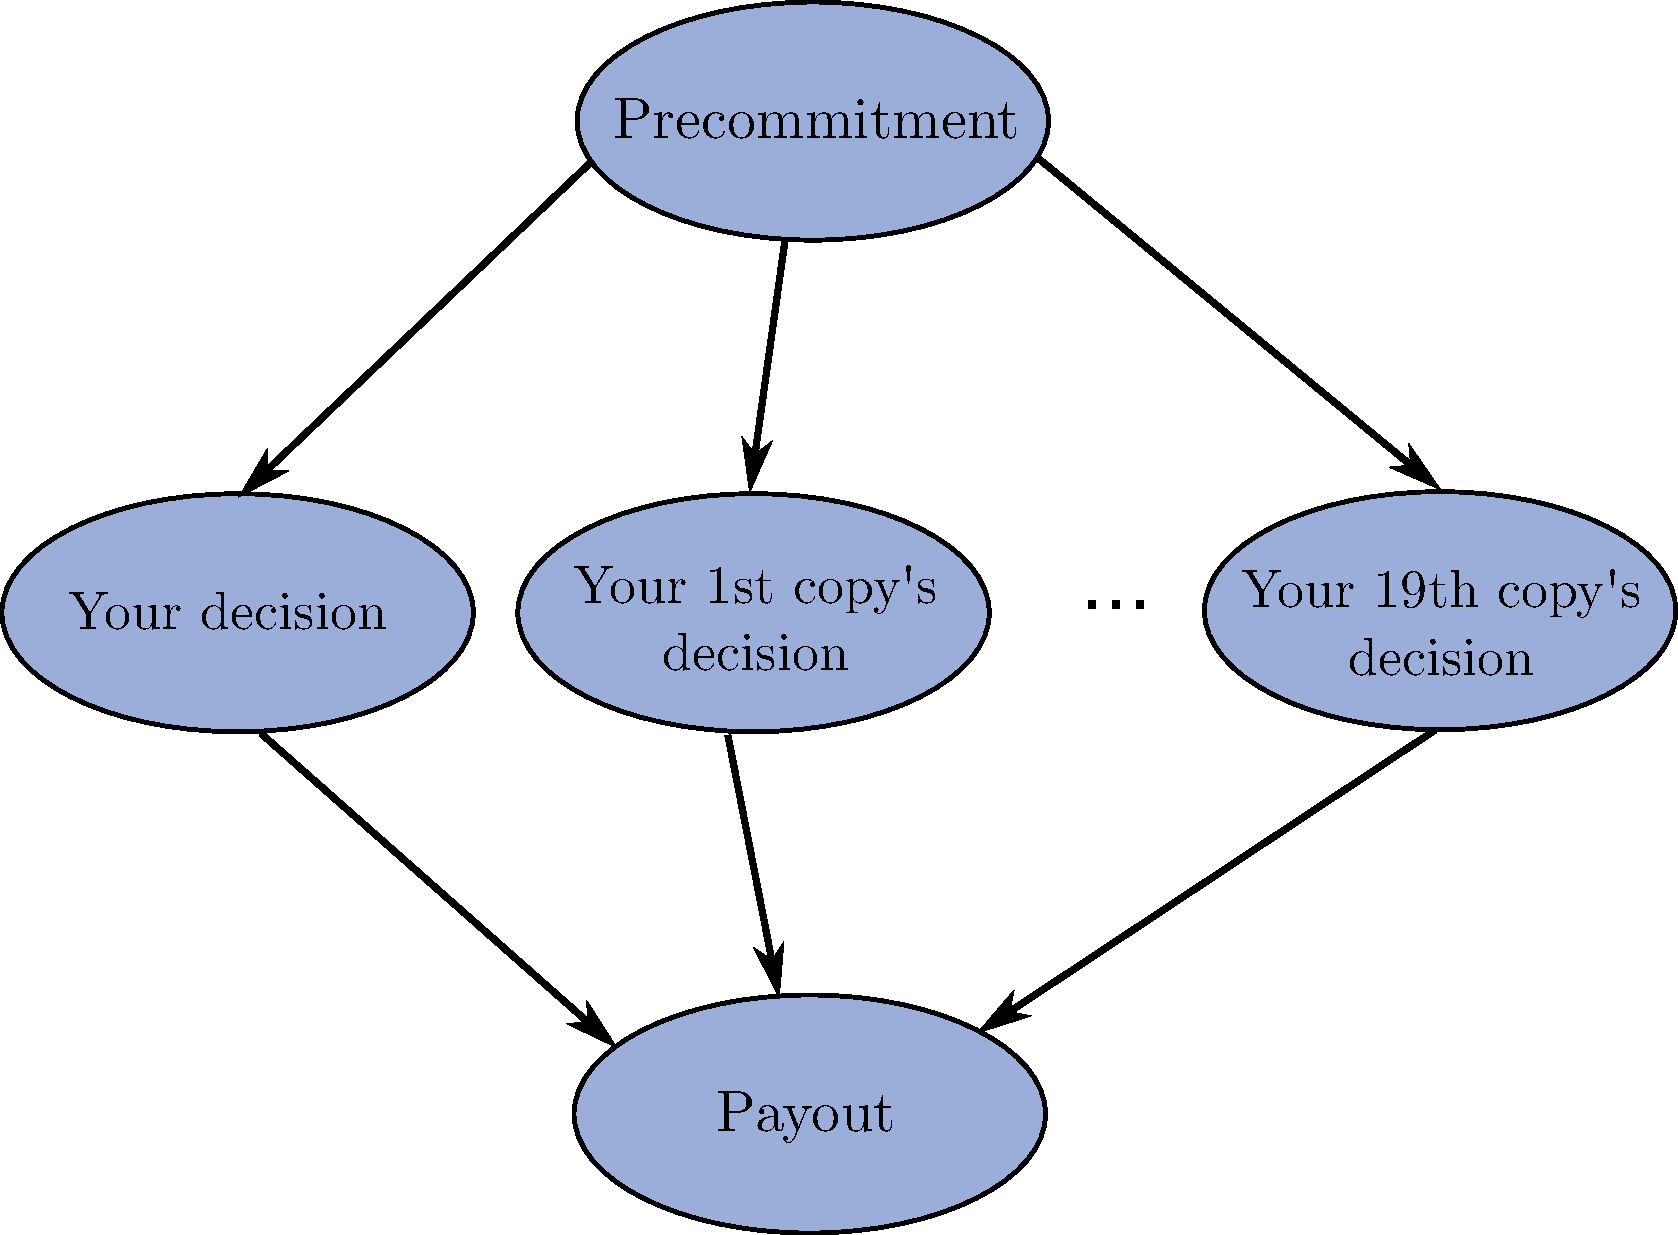
\includegraphics[width=3.46217in,height=2.59375in]{figs/precommitment-causal-graph}
    \caption{A causal graph representing the Donation game with copies and precommitment.}
    \label{precommitment-causal-graph}
\end{figure}


If CDT thinks that it will face some Newcomb-like problem where the copy
or model for prediction is created in the future, it would precommit to
make the same decision that acausal decision theories recommend (without
precommitment). Does that mean that CDT would have to make one
precommitment for each Newcomb-like problem (starting in the future)
that it will face with non-zero probability? Rather than patching its
behavior in each (future) Newcomb-like problem individually, CDT could
also make a more general self-modification. At time \emph{t}, it would
precommit to use the following alternative decision theory in the
future: do what I, at time step \emph{t}, would have precommitted to do
in the present situation
\parencite{Yudkowsky2010-ky,Soares2015-is,Meacham2010-pk}.
Such precommitment is not sufficient to generate the kind of
superrationality required for this paper: it does not cover Newcomb-like
problems that do not start in the future. That is, if the copies are not
created based on a future version of the agent, cooperation with them is
not covered by precommitment. Thus, CDT's precommitment does not imply
cooperation with agents in other parts of the multiverse. However, it
does suffice for a weaker version if we assume the Everett
interpretation of quantum physics (see section
\ref{multiverse-wide-superrationality-for-causal-decision-theorists}).

\hypertarget{lack-of-knowledge-is-evidential-power-part-ii-taking-a-step-back}{\subsection{Lack
of knowledge is evidential power, part II: taking a step
back}\label{lack-of-knowledge-is-evidential-power-part-ii-taking-a-step-back}}

CDT's precommitment only entails partial agreement with its rival
decision theories. Still, it is worth taking a closer look at
precommitment, as it leads us to another interesting dimension along
which decision theories can vary. Consider
\href{https://wiki.lesswrong.com/wiki/Counterfactual_mugging}{Counterfactual
mugging}, also known as ``the curious benefactor''
\parencite{Hintze2014-xs}:

\begin{quote}
\textbf{Counterfactual mugging.} Omega decides to play a game of heads
or tails with you. You are told that if the coin comes up tails, Omega
will ask you to give it \$100. If it comes up heads, Omega will predict
whether you would have given \$100 if the coin had come up tails. If
Omega predicts that you would have given it the money, it gives you
\$10,000; otherwise, you receive nothing. Omega then flips the coin. It
comes up tails, and you are asked to pay \$100. Do you pay?
\end{quote}

If you can precommit to giving the money before you learn about your
poor luck, you should do so. After all, this would render it
near-certain that Omega would give us \$10,000 if the coin comes up
heads, at the mere cost of \$100 if it comes up tails. By precommitting to
pay Omega, we thus gain
$0.5 \cdot \$ 10{,}000  - 0.5 \cdot \$ 100 = \$ 4{,}950$ in
expectation.

A CDT agent would, again, only precommit if Omega bases its prediction on
a future version of the agent, whereas I (and many non-causal decision
theorists) would argue that we should precommit as long as the result of
the coin flip is unknown to us (even if Omega's model is based on a past
version of us).\footnote{In some versions of this problem, Omega has
  already flipped the coin when it approaches you. In those cases, you
  would still win by precommitting long after the coin has already
  landed, provided you are still uncertain about the result of the coin
  flip.} If we do so, we gain information that Omega thinks we give in,
and therefore that we will receive money in expectation. However, once
we learn that the coin came up tails, the ``winning'' move is to keep
the \$100. As before, the problem contains a harmful piece of
information -- although in this case an aspect of the environment, and
not a piece of information about the behavior of other agents, causes
trouble. If we got the chance, we would ``protect'' ourselves against
this piece of information by a precommitment, which renders that piece
of information harmless.

A similar reasoning applies to the Devious postal worker variant of the
donation game: If everyone precommits to cooperation irrespective of
what the postal worker's prediction says, then a negative prediction
about the other agents' behavior can no longer be self-fulfilling. Thus,
if you precommit to cooperating before the postal worker tells you about
the other agents' decisions, you have reason to expect more positive
news (assuming you correlate with the other agents).\footnote{Similar
  lines of reasoning about precommitment apply to thought experiments
  like the Newcomb's problem with transparent boxes
  \parencite{Drescher2006-ky}, retribution
  \parencite{Drescher2006-ky} and
  \href{https://wiki.lesswrong.com/wiki/Parfit\%27s_hitchhiker}{Parfit's
  hitchhiker} \parencite{Parfit1984-ne}.}

As is the case for CDT's precommitment in the previous section, this
leads to a more general self-modification that can be made instead of a
large number of individual precommitments for individual situations.
Specifically, we would (again) precommit to basing our decision in this
situation on what is good from the perspective of the state of knowledge
\emph{prior} to being given new information (like the result of the coin
toss). This is where
\href{https://wiki.lesswrong.com/wiki/Updateless_decision_theory}{updateless
decision theory} gets its name from, and I will call this feature of
decision theories
\href{https://casparoesterheld.com/2016/11/21/thoughts-on-updatelessnes/}{updatelessness}.
Contrary to what the term may suggest, it does not mean that we do not
react to new information at all, but rather that we do it in a different
way. Instead of updating the probabilities we assign to possible states
of the world and making the best decision based on that probability
distribution, we think about what we would have precommitted ourselves
to do in this situation. Usually, what we would have precommitted
ourselves to do is the same as what is then rational for us to do. For
example, if we take a bite from an apple and it tastes foul, we throw
the apple away. If you had to precommit to some action before learning
that the apple is foul, you would also precommit to throw the apple away
if it tastes foul (and to continue eating the apple if it tastes good).
Counterfactual mugging is one of the rare cases in which it does make a
difference.

Acausal decision theorists would precommit to be updateless about all
information they receive in the future. In essence, they would switch to
a decision theory that comes with updatelessness built-in (the most
notable one of them currently being
\href{https://wiki.lesswrong.com/wiki/Updateless_decision_theory}{updateless
decision theory}
\parencite{Benson-Tilsen2014-cv,Hintze2014-xs,McAllister_undated-ms}
itself). Thus, if you had been reasoning about (acausal) decision theory
including the possibility of self-modification correctly all along
(rather than only after learning about the experiment and its result),
you would actually cooperate in the Devious postal worker and give in to
Counterfactual mugging -- even without having precommitted to do so in
these \emph{particular} problems.

Some readers will no doubt already be familiar with updatelessness and
the arguments in favor of it. For those who have not, this may be a good
time to incorporate general updatelessness into their
decision-theoretical intuitions, as it is relevant for some of MSR's
implications (see sections
\ref{updateless-weights}
and \ref{schemes-of-causal-cooperation}).

As a side note, there are justifications of updatelessness that are not
based on precommitment and thus suggest that we should, e.\,g., give the
money in counterfactual mugging even if we previously have not thought
about precommitting to updatelessness. Ryan Carey lists a few in a
\href{https://agentfoundations.org/item?id=1199}{comment} on the
Intelligent Agent Foundations Forum. Benja Fallenstein
\href{http://lesswrong.com/lw/jkm/lzombies_lzombies/}{proposes}
\href{http://lesswrong.com/lw/jpr/sudt_a_toy_decision_theory_for_updateless/}{a
justification} based on ``logical zombies''. For other ideas, see
Armstrong \citeyear{Armstrong2011-sz} and
Drescher \citeyear{Drescher2006-ky}.\footnote{Also note that
  updateless behavior
  \href{https://casparoesterheld.com/2017/05/12/anthropic-uncertainty-in-the-evidential-blackmail/}{can}
  sometimes result from anthropic uncertainty even when applying the
  more classical evidential or causal decision theories.} However, these
are more complicated, non-obvious and not well-established. I thus opted
for limiting myself to the more straightforward precommitment-based
justification for updatelessness as discussed by Meacham~
\citeyear{Meacham2010-pk}, Fallenstein on~\href{http://lesswrong.com/lw/22m/selfmodification_is_the_correct_justification_for/}{LessWrong} and myself in a
\href{https://casparoesterheld.com/2016/11/21/thoughts-on-updatelessnes/}{blog post}
\parencite{Ahmed2012-ue}.

\hypertarget{reasons-and-correlations}{\subsection{Reasons and
correlations }\label{reasons-and-correlations}}

It is difficult to pin down the general principles of how the decisions
of different agents in different situations correlate. Indeed, I suspect
that the problem has no simple solution other than what is implied by
the general solutions to
\href{https://wiki.lesswrong.com/wiki/Naturalized_induction}{naturalized
induction} \parencite{Soares2014-hg,Soares2015-hu} and
decision theory.\footnote{Determining correlations between actions is
  similar to specifying the maxim corresponding to an action in
  \href{https://en.wikipedia.org/wiki/Categorical_imperative}{Kant's
  categorical imperative}. It
  \href{http://briantomasik.com/interpreting-the-categorical-imperative/\#If_everyone_did_what}{seems}
  \href{https://welovephilosophy.com/2013/01/07/choosing-a-kantian-maxim/}{that}
  nobody has a precise grasp of how the latter is supposed to be done
  and that this makes it difficult to apply the categorical imperative.
  However, the problem of specifying the maxim underlying one's action
  does not necessarily have a single correct solution. Determining
  correlations between your actions and that of others, on the other
  hand, follows from any solution to the problems of naturalized
  induction and decision theory. These solutions probably depend on
  priors, but it probably makes more sense to speak of them as having a
  correct solution.}

However, humans seem to have some good intuitions for how decisions
correlate, in part because understanding the correlations between
actions is a day-to-day activity. Imagine seeing your friend Anna being
wounded in her right arm one day. She uses her left arm to apply
bandages and call a doctor, who arrives a few minutes later and inspects
her right arm. A few days later, you see Bob being wounded in his left
arm. Based only on the experience from Anna's wound, what should you
reasonably expect to happen? Will Bob use his left arm to apply bandages
to his right one? Will \emph{Anna} apply bandages to \emph{her} right
arm? Or to Bob's? Will doctors come to Anna? Even after seeing just one
instance of a situation, we are often able to identify many of its
causal links and use this information to infer correlations with similar
situations. If we see the reasons for a decision from the inside, these
correlations become even clearer. If you are Anna and you apply bandages
to your right arm, you know that it is to stop the bleeding. Doing so
gives you no ``weird'' evidence -- it would not lead you to expect, say,
that people are generally likely to apply bandages to things
\parencite{Ahmed2014-ec,Almond2010-xn}.

In general, taking a particular action only because of some reason X
tells you nothing about whether agents who do \emph{not} care (or know)
about X will also take that action.

Importantly, superrationality itself falls under this general rule. That
is, if you do something for superrationality-related reasons, then this
does not tell you anything about how people who do not accept
superrationality would behave. As a trivial example, consider playing a
donation game against 19 people whom you all know to make fun of
superrationality whenever the opportunity avails itself. Attempting to
superrationally cooperate with those people seems rather fruitless.

While these considerations may seem trivial, alleged refutations of
acausal decision theories are often based on ignoring them or assuming
that the evidential thinker ignores them
\parencite{Ahmed2014-ec,Almond2010-xn}.

\subsubsection{Your back is not mine}\label{your-back-is-not-mine}

If the decisions of agents correlate or if each can determine what is
rational, then why can someone -- let us call him Dennis -- not just
determine that it is rational to benefit \emph{him} or his values?
Surely, if everyone just benefited Dennis, that creates the optimal
outcome for him. So, in a donation game with superrationality, perhaps
he should determine the rational policy to be ``cooperate, unless your
name is Dennis''?

This is clearly absurd. The specific reasons that lead Dennis to come up
with this strategy (and to abide by it) do not matter to his fellow
players, although each of them probably have self-serving reasons which
are analogous to those of Dennis. Dennis wants to achieve his own goals,
and this is done optimally if everyone cooperates while he alone
defects. However, this only makes it more likely that some other
participant -- let us call her Dana -- would reason, ``I want to
maximize my payoff; if I could determine everyone's choices, I would
want everyone but \emph{me} (Dana) to cooperate.''
\parencite{Drescher2006-ky}.

\subsubsection{Does accepting superrationality commit us to irrational
behavior in medical Newcomb
problems?}\label{does-accepting-superrationality-commit-us-to-irrational-behavior-in-medical-newcomb-problems}

One common objection to making decisions based on what our action
correlates with, rather than what our action causes, is that it seems to
imply irrational behavior in some cases
\parencite{Nozick1969-op}. In particular, reasoning from
correlation seems to fail in so-called \emph{medical Newcomb problems}.
An example is Yudkowsky's chewing gum
problem~\citeyear{Yudkowsky2010-ul}, which he describes as follows:

\begin{quote}
Suppose that a recently published medical study shows that chewing gum
seems to cause throat abscesses -- an outcome-tracking study showed that
of people who chew gum, 90\% died of throat abscesses before the age of
50. Meanwhile, of people who do not chew gum, only 10\% die of throat
abscesses before the age of 50. The researchers, to explain their
results, wonder if saliva sliding down the throat wears away cellular
defenses against bacteria. Having read this study, would you choose to
chew gum? But now a second study comes out, which shows that most
gum-chewers have a certain gene, CGTA, and the researchers produce a
table showing the following mortality rates:
\end{quote}

\begin{table}[h!]
    \centering
    \begin{tabular} {p{2cm} p{2.5cm} p{2.5cm}}
        \toprule
        & CGTA present & CGTA absent \\
        %\midrule
        \midrule
        Chew gum & 89\% die & 8\% die \\
        Don't chew & 99\% die & 11\% die \\
        %\bottomrule
        \bottomrule
    \end{tabular}
\end{table}

\begin{quote}
This table shows that whether you have the gene CGTA or not, your chance
of dying of a throat abscess goes down if you chew gum. Why are
fatalities so much higher for gum-chewers, then? Because people with the
gene CGTA tend to chew gum and die of throat abscesses. The authors of
the second study also present a test-tube experiment which shows that
the saliva from chewing gum can kill the bacteria that form throat
abscesses. The researchers hypothesize that because people with the gene
CGTA are highly susceptible to throat abscesses, natural selection has
produced in them a tendency to chew gum, which protects against throat
abscesses. The strong correlation between chewing gum and throat
abscesses is not because chewing gum causes throat abscesses, but
because a third factor, CGTA, leads to chewing gum and throat abscesses.

Having learned of this new study, would you choose to chew gum?
\end{quote}

The causal graph of this problem is given in Figure~\ref{causal-graph-CGTA}.
Similar well-known decision problems of this kind are Solomon's problem
\parencite{Gibbard1978-nw,Eells2016-ym}, the Smoking lesion
\parencite{Eells2016-ym}, and the Psychopath button
\parencite{Egan2007-ey}.
\begin{figure}[h!]
    \centering
    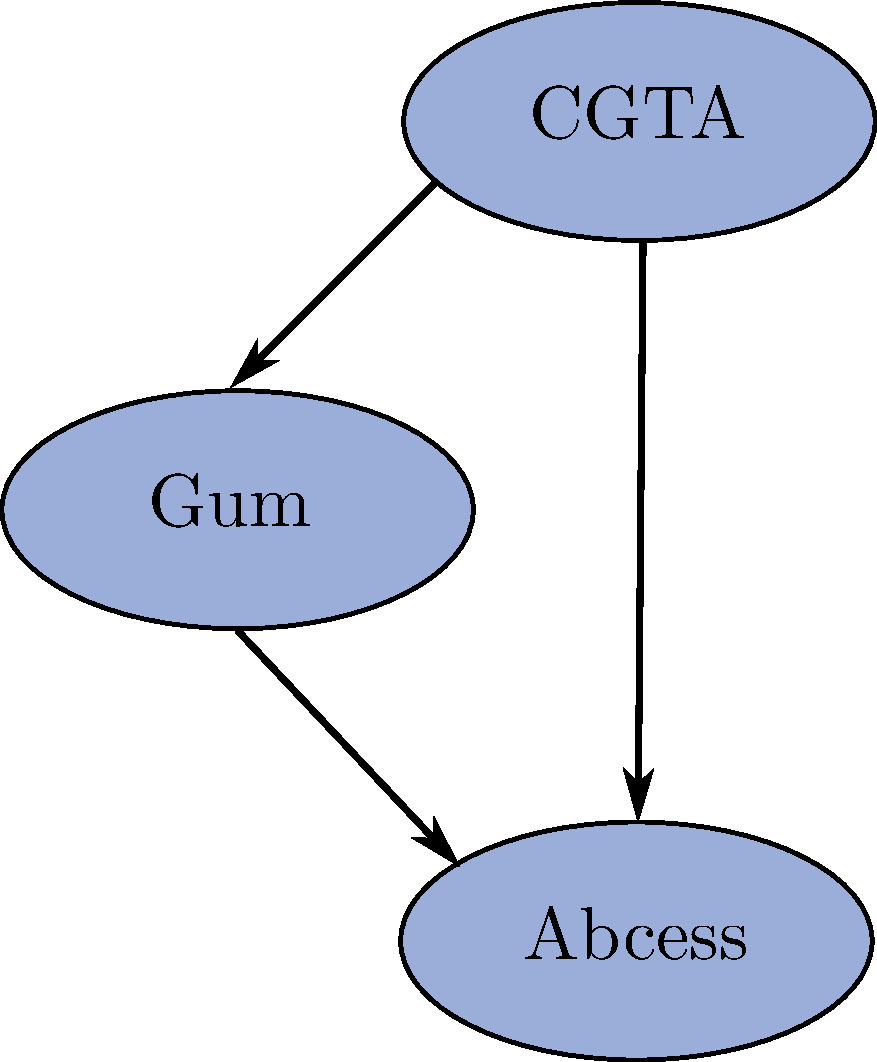
\includegraphics[width=1.95625in,height=2.48452in]{figs/causal-graph-CGTA}
    \caption{A graph representing the causal relationship
in the CGTA thought experiment.}
    \label{causal-graph-CGTA}
\end{figure}
%

Naive correlation-based reasoning suggests that we should still refrain
from chewing gum, since the act of chewing gum would be evidence that we
have the CGTA gene and thus throat abscesses. This strongly conflicts
with our intuition that we should chew gum to protect against the
abscesses. However, I will argue that this provides no convincing
argument against superrationality.

First, the correlation in the Chewing gum problem differs qualitatively
from the correlations between similar decision algorithms~\parencite{OesterheldTreutlein201X}.
%TODOLaTeX
In the Chewing gum problem (and
medical Newcomb problems in general), the correlation stems from a
causal relationship: our genes influence our decisions. Thus, the genes
and the decisions are correlated. The correlations of superrationality,
on the other hand, result from the similarity of the decision
algorithms. The reasoning behind cooperation does not involve a common
cause of all collaborators' decisions. Instead, the correlation may be
viewed as logical \parencite{Garrabrant2016-km}: if I
cooperate, then this implies that all other implementations of my decision algorithm
also cooperate. Figure \ref{two-types} illustrates the difference between
these two types of Newcomb-like problems. Because correlations in
medical and non-medical Newcomb-like problems differ qualitatively,
ignoring the correlations of our actions in the former does not mean we
should ignore them in the latter. In fact, in response to medical
Newcomb problems, philosophers have proposed a variety of decision
theories that behave in this exact way (Treutlein and Oesterheld,
unpublished). That is, they cooperate superrationally (and one-box in
Newcomb's problem) but chew gum in the Chewing gum problem. These
include Spohn's variation of CDT~\citeyear{Spohn2003-zf,Spohn2005-tm,Spohn2012-fo} and Yudkowsky's
timeless decision theory~\citeyear{Yudkowsky2010-ul}.

\begin{figure}[h!]
    \centering
    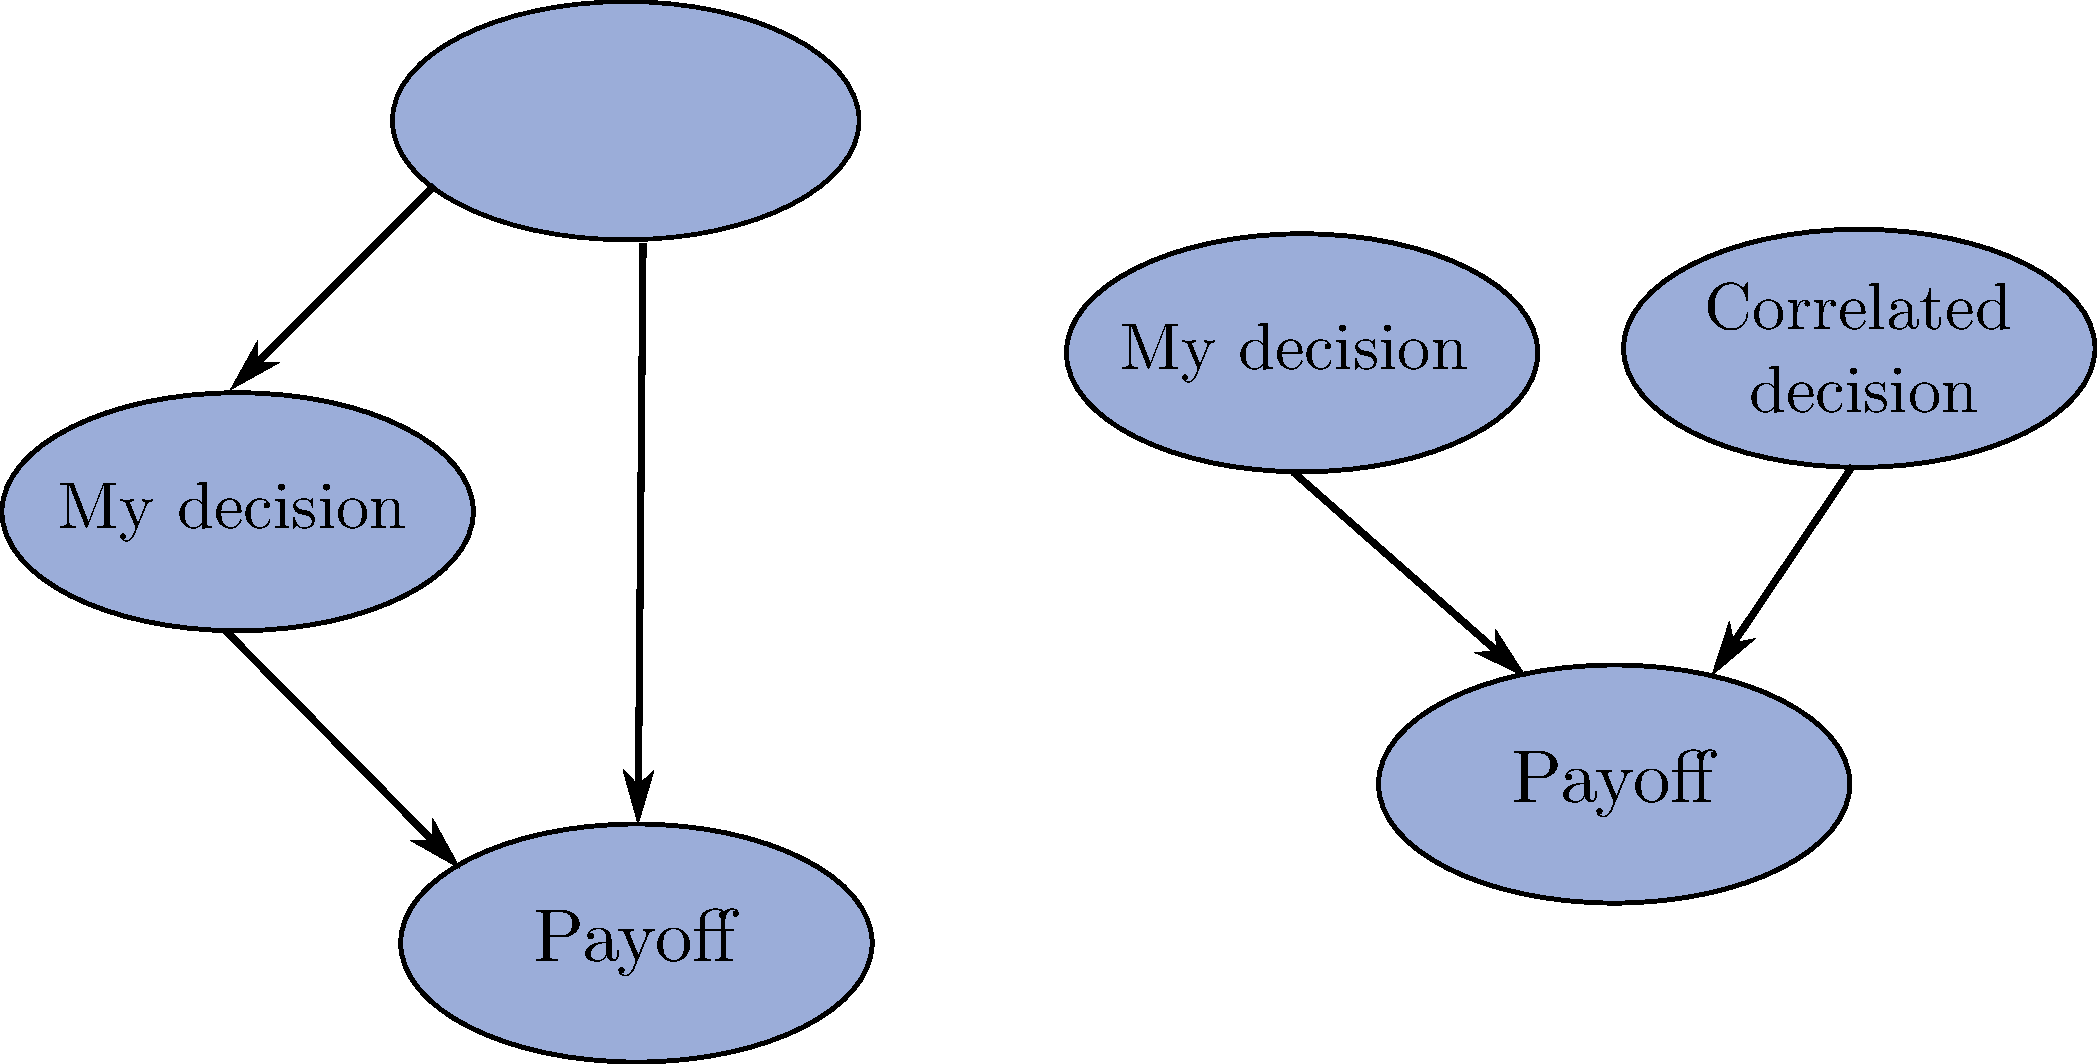
\includegraphics[width=4.1in]{figs/two-types}
    \caption{Generic causal graphs representing the two types of Newcomb-like decision problems. Medical Newcomb problems are illustrated on the left. Newcomb problems based on similarity between decision algorithms are illustrated on the right.}
    \label{two-types}
\end{figure}

Secondly, even purely correlation-based reasoning as done by EDT may
recommend chewing gum, depending on how the causal link from the CGTA
gene to chewing gum is believed to work. Given that people in the study
presumably did not know that chewing gum helps against throat abscesses,
it is plausible that CGTA causes people to intuitively desire chewing
gum. However, if learning about the study and applying EDT then causes
us not to chew gum, it does not tell us anything about whether having
the CGTA gene would have caused us to do the opposite. Similarly, if you
know that a sprinkler has watered the lawn, observing that the grass is
wet is no evidence that it has also rained (see Figure
\ref{tickle-defense}). The sprinkler already explains why the lawn is wet,
so you do not need rain as an additional explanation
\parencite{Ahmed2014-ec}.


\begin{figure}[h!]
    \centering
    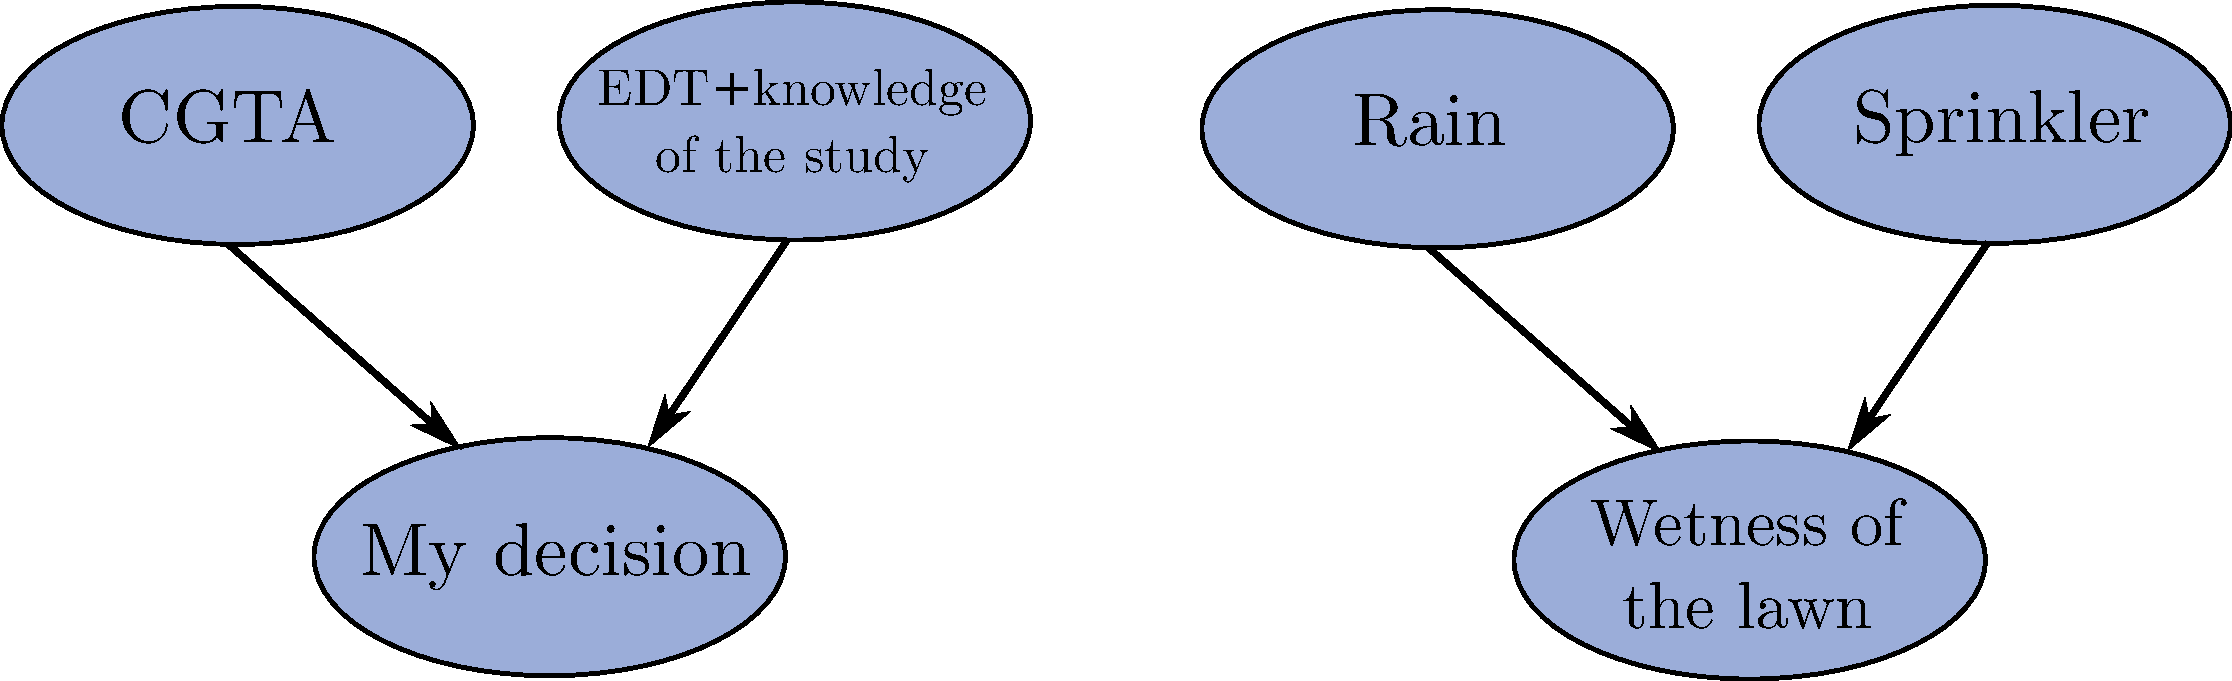
\includegraphics[width=4.09792in,height=1.27975in]{figs/tickle-defense}
    \caption{If you decide not to chew gum after applying EDT
to your knowledge of the study, it may tell you as much about whether
you have the CGTA gene as seeing a lawn watered by a sprinkler tells you
about whether it has rained.}
    \label{tickle-defense}
\end{figure}

\hypertarget{are-the-correlations-strong-enough}{\subsection{Are the
correlations strong enough?}\label{are-the-correlations-strong-enough}}

In most superrationality-related thought experiments, it is assumed that the
other agents are near-copies of ours. The problems presented in this
paper are no exception. However, in any real-world setting, most agents
are not close copies of ours. We should therefore expect correlations to
be much less than perfect.

Luckily, the total number of agents in the multiverse is probably so
vast\footnote{In fact, most multiverse theories contain infinitely many
  agents. This leads to some additional complications, discussed in
  section \ref{infinite-ethics}.} that the correlations between ourselves and any
\emph{individual} agent need not be very large\footnote{Decision
  theorists have picked up on the point that large numbers of agents can
  bring out the differences between CDT and EDT in realistic cases. In
  particular, large elections are often mentioned as such a case
  \parencite{Ahmed2014-ec}.} (see section
\ref{many-agents}). Because many
agents probably do not know about superrationality, we may assume that
99.99\% of the agents do not correlate with us at all when it comes to the decision whether to cooperate superrationally. In this case,
cooperation with the rest still pays off if we believe that our
correlation with the others is non-negligible and positive. It does not
matter that we inadvertently benefit many ``free riders''. For example:
if our cooperation makes it 1\% more likely that each of these
correlated agents also cooperates, then if there are ``only'' a billion
of them, we can expect 10 million more to cooperate if we
cooperate.\footnote{Note that this is usually not an instance of
  \href{https://wiki.lesswrong.com/wiki/Pascal\%27s_mugging}{Pascal's
  mugging}, although the underlying mathematical mechanism (multiplying
  very small numbers with very large numbers) is similar. Whereas in
  Pascal's mugging, a big reward outweighs the low probability assigned
  to it, multiverse-wide superrationality (MSR) involves a low
  probability being outweighed by the large number of near-independent
  instances of that probability. The positive result occurs with a high
  probability as long as the other agents' decisions of whether to
  cooperate are mostly independent of one another. For comparison,
  imagine drawing balls out of a box containing 1,000,000 balls. You are
  told that the probability of drawing a blue ball is only 1/1,000 and
  that the probabilities of different draws are independent. Given this
  information, you can tell with a high degree of certainty that there
  are quite a few blue balls in the box. Multiverse-wide correlations
  between agents thus becomes much more important to consider than the
  correlations in smaller scale problems like the donation game, unless
  we are skeptical of some of the underlying assumptions.}

\subsubsection{Correlation only with close
copies?}\label{correlation-only-with-close-copies}

Some might think that they are uncorrelated with everyone else apart
from very close copies of themselves. Because such near-copies would
likely share their utility function to a large extent, there is no need
to cooperate with them (although coordination
\protect\hyperlink{notes-on-superrational-coordination}{may be} useful,
depending on the utility function, see section
\ref{notes-on-superrational-coordination}). While the lack of formalized and
agreed-upon solutions to decision theory and naturalized induction
\parencite{Soares2014-hg,Soares2015-hu} makes it difficult
to draw definitive conclusions on such matters, I am nevertheless
skeptical of this objection to MSR. It seems to me that decision
theories, at least as people currently conceive of them, are compatible
with very large sets of possible minds. That is, if an agent uses, say,
evidential decision theory, it can still use all kinds of different
mechanisms for assigning conditional probabilities and, most
importantly, it can still have all kinds of values (see section
\ref{orthogonality-of-instrumental-rationality-and-values}).

\hypertarget{negative-correlations}{\subsubsection{Negative
correlations?}\label{negative-correlations}}

There is another interesting objection about correlation strength that
could be raised: perhaps we should expect to correlate \emph{negatively}
with some agents in the multiverse, such that cooperation can even do
some harm (beyond the opportunity costs connected to it) as it makes
some other agents more likely to defect. While interesting, I do not
find this reason against superrational cooperation very convincing,
either.

First, we have to consider what negative correlation means. Let's say
you currently think that roughly 0.1\% of evolved agents in the
multiverse who have thought about MSR decide to cooperate. Now, you
learn of one randomly chosen agent that she cooperates. The intuitive
response is to increase the 0.1\% estimate, if only slightly (depending
how confident you were in your initial estimate). If this agent were
\emph{negatively} correlated with the others, then upon learning that
this one agent cooperated, you would adjust your estimate of how many
agents cooperate \emph{downward}.

Such a reaction seems implausible given our state of knowledge. Surely,
there are a few eccentric agents who have superrationality-related
algorithms similar to mine, yet choose to somehow invert the output of
these algorithms. But such algorithms make little sense from an
evolutionary point of view and so I do not expect them to be very common
in the multiverse.

It may seem that agents have an incentive to become negatively
correlated (via self-modification), thereby enabling them to defect and
make everyone else cooperate. However, there are various problems with
this idea. For one, to be able to correlate negatively with the other
agents it seems as though one would have to find out about their
decision and then do the opposite, which appears to be difficult.
Furthermore, self-modification also commits us to cooperate more when
the others defect -- an agent committed to unconditional defection does
not correlate with anyone else.

The intuition underlying the self-modification idea is that by
self-modifying to be negatively correlated, we can acausally determine
the others' decisions. But I do not think this works in the relevant
way. When you modify your decision algorithm, you lay your power into
the hands of the new algorithm. This means you cannot, for example,
self-modify to some decision algorithm A that does the exact opposite of
what everyone else is doing, and then defect -- unless A already
defects on its own. Thus, you cannot determine everyone else to
cooperate unless you are already correlated with them. Similarly, you
cannot commit to output the 100th digit of $\pi$, and then return 6 anyway
to acausally determine the value of $\pi$. However, if you are already
correlated with the 100th digit of $\pi$, you can logically determine its
value. For instance, if Omega predicts your behavior and then tells you
that if you raise your arm, the 100th digit of $\pi$ will be 7 and if you do
not it will be 1, you can determine the 100th digit of $\pi$. Of course,
these stop working once you know what the 100th digit of $\pi$ is.

As a last point, self-modification does not seem to add anything to
direct defection (without self-modification). To see why, let us
consider the two kinds of agents that are not yet negatively correlated
with the others. The first agent is not correlated with others before
self-modification, and therefore has no reason to self-modify. He can
just defect directly, without adopting a weird decision theory that is
about doing the opposite of what someone in some other part of the
multiverse is doing. The second agent is (positively) correlated with
others before self-modification. Her problem is that if she
self-modifies, others will do so as well, which gives her evidence that
a lot more defection is happening than if she would cooperate.

Another relevant point is that there is a sharp upper bound to the
amount of negative correlation that can exist within a group of agents.
Imagine agents A, B, and C, whose decision to cooperate we model as a
random variable with the two values 1 (for cooperation) and 0 (for
defection). Let us say A is perfectly negatively correlated with B and B
is perfectly negatively correlated with C. A is then perfectly
\emph{positively} correlated with C. So, even among just three agents,
not all correlations can be perfect and negative. On the other hand, the
pairwise correlations may well all be perfect and \emph{positive}. To
study this further, we move from correlations to
\href{https://en.wikipedia.org/wiki/Covariance}{covariances},
because they
\href{https://en.wikipedia.org/wiki/Covariance\#Properties}{can}
be meaningfully added up. In general, we
\href{https://casparoesterheld.files.wordpress.com/2017/01/lowerboundavgcov.pdf}{can
derive} a lower bound of \(- \frac{1}{4(n - 1)}\) for the average
covariance between pairs of agents from any set of \(n \geq 2\) agents
(excluding ``pairs'' of one and the same physical agent), if cooperation
is seen as a binary
\href{https://en.wikipedia.org/wiki/Random_variable}{random variable}.
If the agents are all perfectly correlated, then all covariances are at
most \(\frac{1}{4}\), so the \emph{upper} limit for the average
covariance is also \(\frac{1}{4}\).
\href{https://en.wikipedia.org/wiki/Mediocrity_principle}{Unless
we have reason to believe that we are special}, i.\,e. that our
covariance with the others falls far below the average covariance
between two agents, this suggests that especially for very large numbers
of agents \(n\), our possible acausal impact under the assumption of
only positive covariances can be much larger than that of negative
covariances. In fact, the covariances of the average agent cannot add up
to something below \(- \frac{1}{4}\) regardless of the number of agents.
In contrast, they can be as high as \(\frac{1}{4}(n - 1)\) for positive
covariances. If we
\href{https://casparoesterheld.com/2016/10/21/environmental-and-logical-uncertainty-reported-environmental-probabilities-as-expected-environmental-probabilities-under-logical-uncertainty/}{view
the covariances as uncertain}, this suggests a prudential argument in
favor of assuming positive covariances to dominate over negative ones,
given that our acausal influence is so small under the opposite
assumption. However, the details of this argument (and whether it works
at all) depend on our ``meta-probability distribution'' over
covariances.

\hypertarget{the-relative-importance-of-superrational-cooperation-an-example-calculation}{\subsection{The
relative importance of superrational cooperation: an example
calculation}\label{the-relative-importance-of-superrational-cooperation-an-example-calculation}}

Looking at a single decision, how do the benefits from superrational
cooperation compare with the opportunity costs? Although we need to make
some unrealistic assumptions (such as exact symmetry of the decisions
faced by all the agents) in order to calculate this value, it is
nevertheless worth an attempt, if only for the purpose of illustration.

We assume that there are \(n\) superrational agents whose decisions in
donation games are perfectly correlated; that is, either all of them
cooperate or all of them defect. Realistically, many more agents'
decisions will correlate weakly with ours, while only very few
correlations will be perfect. However, the implications of many weak and
a few strong correlations are similar. For simplicity, we assume that
the goals of the agents are orthogonal to each other, i.\,e. that if
someone benefits it is neutral in expectation to any other value system.
All of them have values that can benefit from behavior in other
universes to the same extent.

The \(n\) agents face the decision between a) generating \(b_{u}\)
\href{https://en.wikipedia.org/wiki/Cardinal_utility}{cardinal},
\href{https://en.wikipedia.org/wiki/Social_choice_theory\#Interpersonal_utility_comparison}{interpersonally
comparable} utils (or utilons) for their own utility function and b)
generating \(b_{\text{other}}\) utils for \(k\) randomly chosen
superrationalists.

Choosing option a) makes everyone chose option a) and so only generates
\(b_{u}\) utils for us. Choosing option b) makes everyone choose option
b). Whenever someone (including ourselves) chooses option b), there is a
probability of \(\frac{k}{n}\) that we are among the beneficiaries.

Overall, if we and thus everyone else chooses option b), we receive \(n\frac{k}{n}b_{\text{other}} =
kb_{\text{other}}\) utils. Choosing option b) is therefore to be preferred if and only if
\begin{equation}
kb_{\text{other}} > b_{u}.
    \label{eq:preferred}
    % previously (*)
\end{equation}

This suggests that our own preferences have no priority over those of
other superrationalists in this decision. We only decide based on ``the
greatest good for the greatest number''. For instance, if \(k = 1\),
then we should choose option b) to help other value systems if
\(b_{\text{other}} > b_{u}\), i.\,e. as long as helping other value
systems can be done more efficiently than helping your own values. This
shows how important superrationality considerations can be. Whereas the
non-superrational agent maximizes only for its own value system, the
superrational agent maximizes for the value systems of other
superrational agents just as much as for their own.

Moreover, whether we cooperate depends only on the number of agents
whose cooperation is correlated with ours and not at all on the number
of agents that will defect. In this regard, multiverse-wide
superrational cooperation differs from most causal cooperation, where we
usually try to ensure that beneficiaries of our actions reciprocate
(unless we care about them intrinsically).

As mentioned already, this analysis is based on unrealistic assumptions
of perfect symmetry to highlight the relative importance of
superrationality considerations. We will now move on to more general,
potentially asymmetric cases.

\hypertarget{compromise-strategy}{\subsection{Compromise
strategy}\label{compromise-strategy}}

\subsubsection{Sharing gains from compromise in the face of
asymmetries}\label{sharing-gains-from-compromise-in-the-face-of-asymmetries}

We have so far only considered completely symmetrical situations,
wherein other agents faced the exact same decision problem as ourselves.
One could either choose to cooperate, which correlated with everyone
else's cooperation; or defect, which correlated with everyone else's
defection. Both cooperation and defection were associated (via the
correlation between agents) with particular outcomes. Based on these
correlations it was straightforward to choose the action that correlates
with the best outcome for ourselves (and also for everyone else). Of
course, in practice, compromise will not be this tidy. Specifically, we
will have to deal with asymmetrical decision problems. Consider the
following example:

\begin{quote}
\textbf{Superrational
\href{https://en.wikipedia.org/wiki/Fair_cake-cutting}{cake
cutting}.} You are playing a donation game with two fellow players
whose decision algorithms correlate strongly with yours. Unlike other
donation games, the currency in this game is cake, of which there are
two flavors -- vanilla and strawberry. Each player's utility grows in
linear proportion to how much cake they eat, and they all have taste
preferences that affect their total utility. Let's say you, player 1,
like vanilla twice as much as strawberry. Player 2, meanwhile, likes
strawberry four times as much as vanilla, and player 3 likes both
flavors equally. Each player currently owns different amounts of
strawberry and vanilla cake. You have one strawberry cake and one
vanilla cake, while player 2 has three vanilla cakes and player 3 has
one strawberry cake. (See Figure
\ref{Superrational-cake-cutting} for an illustration of
these circumstances.) You all know each other's taste preferences and
can send arbitrary fractions of your cakes to one another, but none of
you are allowed to communicate. You only get to send one box of cake to
each player, and you receive your boxes from them after you've sent
yours. What should you do?
\end{quote}

\begin{figure}[h!]
    \centering
    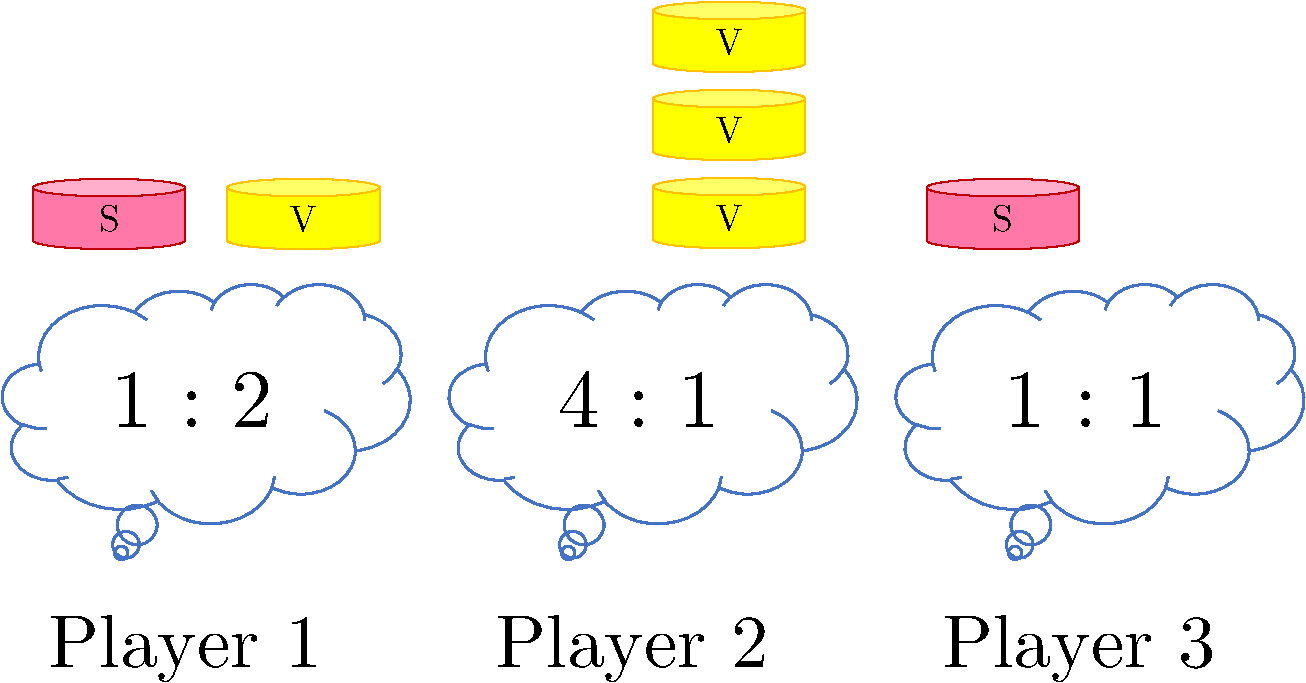
\includegraphics[width=4in]{figs/Superrational-cake-cutting}
    \caption{An overview of property and preferences in the Superrational cake cutting.}
    \label{Superrational-cake-cutting}
\end{figure}

First note that this problem is indeed one of superrational cooperation.
If causal decision theory is applied, then the dominant strategy for
each player is to keep all the cake -- but this would be a suboptimal
outcome for everyone. The players have two strawberry and four vanilla
cakes in total. If you could redistribute them so that player 1 has one
strawberry and two vanilla cakes, player 2 has one strawberry cake, and
player 3 has two vanilla cakes, everyone would be better off than
without any redistribution. However, there are infinitely many
other possible (fractional) distributions that would also be better for
everyone. This makes it hard to decide among them.

One part of the problem is that it is unclear what our decisions
correlate with. If we send player 2 a piece of her preferred cake
(strawberry), can we expect to get some of our preferred cake (vanilla)
from her? If so, how much? If we could pin down the correlations and
assign probabilities to each combination of strategies -- i.\,e. to each
\href{https://en.wikipedia.org/wiki/Strategy_(game_theory)}{strategy
profile} -- conditional on any of our actions, we could choose the
action that maximizes expected utility (the exact formulation of which
depends, of course, on our decision theory). But even if the agents know
that they have very similar (or even identical) decision algorithms, the
asymmetries make it hard to assign these probabilities.

Another perspective on the problem is that asymmetries make it unclear
who ``deserves'' how much. In the symmetrical situations it was always
clear that everyone should get the same, but this is different in
superrational cake-cutting.

It is useful to view the symmetry of a compromise problem as a
non-binary property. For example, a donation game in which one player
gains slightly more than the others from cooperating may still be
symmetric enough to make it obvious what the right decision is.

\hypertarget{the-compromise-problem}{\subsubsection{The compromise
problem}\label{the-compromise-problem}}

In order to solve the problem of superrational compromise in asymmetric
situations, we will treat compromise as a game-theoretical problem. Note
that this requires basic knowledge of game theory; for an introduction
see, e.\,g. \citet{Osborne2004-ui}. Formally, a game
consists of

\begin{itemize}
\item
  a finite set of players \(P = { p_{1},\dotsc,p_{n}}\),
\item
  for each player \(p_{i}\), a set of actions \(A_{i}\),
\item
  for each player \(p_{i}\) a utility function
  \(u_{i}\colon A_{1} \times \dotsm \times A_{n} \rightarrow \mathbb{R}\), where
  \(\mathbb{R}\) refers to the real numbers. 
\end{itemize}

Multiverse-wide superrational compromise is a game where \(P\) is the
set of correlated superrationalists, the utility functions \(u_{i}\)
represent their preferences, and the sets of possible actions \(A_{i}\)
represent the set of strategies a player can pursue in their part of the
multiverse. Note that the last aspect of the definition assumes that the
players' preferences are
\href{https://en.wikipedia.org/wiki/Von_Neumann\%E2\%80\%93Morgenstern_utility_theorem\#The_axioms}{von
Neumann-Morgenstern-rational} (vNM-rational), which is technically
useful and mostly non-controversial\footnote{One exception may be the
  axiom of continuity. It is violated by preferences with lexicality,
  which are commonly discussed in moral philosophy
  \parencite{Knutsson2016-kd}. However, if we drop the axiom
  of continuity,
  \href{https://casparoesterheld.com/2016/08/08/lexicographic-utility-functions/}{we
  can} still represent the preferences as a lexicographic utility
  function \parencite{Blume1989-fd,Fishburn1971-bx}.
  However, a treatment that includes lexicographic utility functions is
  beyond the scope of the present paper. Because in uncertain
  situations, a lexicographic utility function is usually equivalent to
  only maximizing the lexically highest values, we may nonetheless apply
  the present results by simply omitting all lexically lower values.}.

Our notation indicates that utilities are calculated deterministically
from action tuples. However, we will sometimes view the utilities
\(u_{i}(a_{1},\dotsc,a_{n})\) as random variables in the
\href{https://en.wikipedia.org/wiki/Bayesian_probability}{Bayesian
sense}. This is because we are usually uncertain about the implications
of the policies \(a_{1},\dotsc,a_{n}\), as well as the utility function
\(u_{i}\) itself, in the context of MSR.

Now, the question is which (potentially
\href{https://en.wikipedia.org/wiki/Strategy_(game_theory)\#Mixed_strategy}{mixed})
strategy \(\alpha_{i}\) any player \(p_{i}\) should choose. Note that we
are not looking for the (CDT-based) Nash equilibria of the game. We will
therefore have to move our focus from (Nash equilibrium-based)
\href{https://en.wikipedia.org/wiki/Non-cooperative_game_theory}{non-cooperative}
to
\href{https://en.wikipedia.org/wiki/Cooperative_game_theory}{cooperative
game theory}.

In principle, the optimal strategy \(\alpha_{i}^{*}\) can be determined
by applying one's decision theory. For example, if one were to use EDT,
then the optimal strategy is
$$
\argmax_{\alpha_{i}}\ \mathbb{E}\lbrack u_{i}(a_{1},\dotsc,a_{n})\mid \alpha_{i}\rbrack.
$$
As noted earlier, however, computing or optimizing the expected value
conditional on one's action directly is not feasible in situations of
asymmetric payoffs. To find the best action, we will therefore
approximate the above expected value maximization with some new
criterion, similar to how game theory has replaced expected value
maximization with Nash equilibria and other concepts.

We will therefore try to develop some new \emph{compromise utility
function} \(u^{*}\colon A_{1} \times \dotsm \times A_{n} \rightarrow \mathbb{R}\),
intended as a new criterion for choosing the optimal strategy. Because
the compromise utility function depends less on the specifics of the
problem, it will prove to be easier to reason about what the adoption of
some \(u^{*}\) tells us about what the other agents do. The optimal
\(u^{*}\) can then, under certain assumptions, tell us what action to
take. At least if our choosing \(u^{*}\) means that everyone else
chooses the same \(u^{*}\) (which is not necessarily the case), then
player \(p_{i}\) should implement the \(i\)-th strategy entry of
$$
\argmax_{(\alpha_{1},..,\alpha_{n}) \in A_{1} \times \dotsm \times A_{n}}\ \mathbb{E}\lbrack u^{*}(\alpha_{1},\dotsc,\alpha_{n})\rbrack.
$$
Once again, having a compromise \emph{utility function,} as opposed to
more general compromise \emph{preferences}, implicitly assumes that the
compromise preferences are also vNM-rational.

\hypertarget{cooperation-with-and-without-coordination}{\subsubsection{Cooperation
with and without
coordination}\label{cooperation-with-and-without-coordination}}

In a way, \(\argmax_{(\alpha_{1},..,\alpha_{n}) \in A_{1} \times \dotsm \times A_{n}}
\mathbb{E}\lbrack u^{*}(\alpha_{1},\dotsc,\alpha_{n})\rbrack\) is the optimal plan on the assumption
that everyone will follow it. With practical degrees of correlations, however, we cannot assume that
everyone will arrive at the same plan, especially if multiple plans have
the same compromise utility. In MSR, it is especially unlikely that
everyone will arrive at the same plan, as superrational collaborators
have different states of knowledge about the multiverse and each others'
value system.

A perfect plan may have catastrophic results if it is not accurately
followed by everyone involved. Specifically, plans are risky if the
utility of one player's action hinges on another player's action because
such plans assume the ability to coordinate. Hence, it is useful to look
at a class of utility functions where coordination plays no role.

We say that a utility function \(u_{i}\) \emph{(additively) decomposes
into local utility functions}
\(\{ u_{i,j}\colon A_j \rightarrow \mathbb{R}\}_{j = 1,\dotsc,n}\) if
$$
u_{i}(a_{1},\dotsc,a_{n}) = \sum_{j=1}^n u_{i,j}(a_{j}).
$$

Intuitively speaking, \(u_{i}\) decomposing into local utility functions
means that any player \(p_{j}\) has a very direct impact on \(p_{i}\)'s
utility, such that when \(p_{j}\) attempts to benefit \(p_{i}\) she need
not think about what other players do.

In game theory as it is usually applied to interactions between agents
on Earth, the assumption of additive decomposition of utility functions
would be a severe limitation: if agents interact with each other
physically, then, of course, the impact of an action often depends on
the other players' actions. As examples, consider some of the classic
games studied in game theory, such as
\href{https://en.wikipedia.org/wiki/Battle_of_the_sexes_(game_theory)}{Bach
or Stravinsky} or
\href{https://en.wikipedia.org/wiki/Chicken_(game)}{Chicken}.

In the problem of multiverse-wide compromise, on the other hand, there
is probably no causal interaction between the actions of agents in
different parts of the multiverse. Additive decomposition of utility
functions is thus a more natural assumption in this context. That said,
issues of coordination can still arise in the utility function itself.
As an example, consider a utility function that wants there to be at
least one (dis-)proof of the
\href{https://en.wikipedia.org/wiki/Riemann_hypothesis}{Riemann
hypothesis} somewhere in the multiverse, but does not care about the
existence of further, redundant proofs. This utility function does not
decompose additively; whether I benefit this utility function by proving
the Riemann hypothesis depends on whether someone else is already
working on a proof. Other, perhaps more realistic, examples of ethical
notions that do not decompose into local utility functions are (partial)
\href{https://en.wikipedia.org/wiki/Average_and_total_utilitarianism}{average
utilitarianism} and potentially
\href{https://en.wikipedia.org/wiki/Biodiversity}{biodiversity}.
However, many other plausible utility functions (e.\,g., total
utilitarianism) do fulfill the above condition.

If some of the utility functions in a game do not decompose into local
utility functions, we will call the game a \emph{coordination
problem}\footnote{This differs somewhat from more standard
  game-theoretical definitions of coordination. For a discussion of the
  relationship, see \parencite{Oesterheld2017-lt}.}.
Theoretically, the following arguments also work for coordination games,
but they are much more robust and practically applicable in problems
that require little or no coordination. This topic will be discussed
further in section
\ref{notes-on-superrational-coordination}.

\subsubsection{Harsanyi's aggregation
theorem}\label{harsanyis-aggregation-theorem}

Although we do not yet know how and to what extent, we know that our
compromise utility function \(u^{*}\) should incorporate the utility
functions \(u_{1},\dotsc,u_{n}\) but not be sensitive to anything else. The
following assumption captures these attitudes:

\vspace{3mm}

\begin{assumption}
\label{ass:compromise_util}
Let P and Q be probability distributions over outcomes \(A_{1} \times
\dotsm \times A_{n}\) such that \(\mathbb{E}_{P}\lbrack u_{i}(a_{1},\dotsc,a_{n})\rbrack \geq
\mathbb{E}_{Q}\lbrack u_{i}(a_{1},\dotsc,a_{n})\rbrack\) for \(i = 1,\dotsc,n\).\footnote{This notation --
    viewing the lotteries as probability distributions over action vectors -- is a bit unnatural,
    and stems from the lack of an intermediate step of world states or histories between action
    vectors and utilities in our notation. If we extended our notation with such an intermediate
    step, then the lotteries would be over states of the world rather than action vectors. Although
the proofs also work with action vectors, it may help to think of the lotteries as being over
histories.} That is, all players like P at least as much as Q. Then \(\mathbb{E}_{P}\lbrack
u^{*}(a_{1},\dotsc,a_{n})\rbrack \geq \mathbb{E}_{Q}\lbrack u^{*}(a_{1},\dotsc,a_{n})\rbrack\), i.\,e. the
compromise utility function also values \(P\) at least as highly as \(Q\).
\end{assumption}

We could view this assumption as a decision to limit ourselves to a
particular class of compromise utility functions -- a decision that
makes our superrational collaborators limit themselves to the same
class. In terms of expected value for ourselves, this is a good
decision. It basically does not tell us anything other than that we do
not want to pay anything to switch from P to Q if everyone likes P at
least as much as Q.

We furthermore introduce the notion of utility function equivalence: two
utility functions \(u\) and \(v\) are equivalent, written as
\(u \sim v\), if they imply equal behavior. For the
\href{https://en.wikipedia.org/wiki/Cardinal_utility}{cardinal
utility functions} discussed here, this is the case if one arises from
positive affine transformation of the other, i.\,e. if \(u = av + b\) for
some \(a \in \mathbb{R}_{> 0}\) and \(b \in \mathbb{R}\).

Assumption~\ref{ass:compromise_util} does not seem especially strong, but it turns out that it
suffices for a significant result regarding the shape of the compromise utility function. It is
essentially a version of Harsanyi's aggregation theorem (\cite{Harsanyi1955-ou}; see also
\cite{Peterson2017-pa}, section 13.4 for an introduction).\footnote{Interestingly, the proof of the
    aggregation theorem given by \citet{Harsanyi1955-ou} contains an error. However, since then
    a few alternative, correct proofs have been published
    \parencite{Fishburn1984-zh,Border1985-mw,Hammond_undated-bp}.}

\begin{theorem}
\parencite{Resnik1983-hl,Fishburn1984-zh} Let \(u^{*}\) be
a compromise utility function for \(u_{1},\dotsc,u_{n}\) that satisfies
Assumption B. Then there are weights
\(\lambda_{1},\dotsc,\lambda_{n} \in R_{\geq 0}\) such that
\begin{equation}
    u^{*} \sim \sum_{i=1}^n\lambda_{i}u_{i}.
    %previously (**)
    \label{eq:weights}
\end{equation}
    \label{th:compromise}
\end{theorem}

Note that the \(\lambda_{i}\) are not unique. Also, not all weight
assignments consistent with Eq.~\eqref{eq:weights} or Assumption~\ref{ass:compromise_util} have only positive
weights. In particular, if \(u_{i} = u_{j}\) for some \(i \neq j\), we
can decrease \(\lambda_{i}\) by an arbitrary constant \(C\) if we
correspondingly increase \(\lambda_{j}\) by \(C\), and end up with the
same compromise utility function \(u^*\).
\parencite{Resnik1983-hl,Fishburn1984-zh}. If
\(C > \lambda_{i}\), we arrive at an equivalent utility function that
assigns negative weights.


\begin{theorem}
Let \(u_{1},\dotsc,u_{n}\) each decompose into local utility functions \(\{{ u}_{i,j}\colon A_{j} \rightarrow
\mathbb{R}\}_{j = 1,\dotsc,n}\).  Then a compromise utility function \(u^{*}\) that satisfies
Assumption~\ref{ass:compromise_util} relative to \(u_{1},\dotsc,u_{n}\) also decomposes into local
utility functions.
    \label{th:decompose}
\end{theorem}

\begin{proof}
Because of Theorem \ref{th:compromise}, it is 
\begin{equation*}
    \begin{split}
        u^{*}(a_{1},\dotsc,a_{n}) &= b + \sum_{i=1}^n\lambda_{i}u_{i}(a_{1},\dotsc,a_{n}) \\
                               &= b + \sum_{i=1}^n\lambda_{i}\sum_{j=1}^nu_{i,j}(a_{j}) \\
                               &= b + \sum_{j=1}^n\sum_{i=1}^n\lambda_{i}u_{i,j}(a_{j}) \\
                               &= \sum_{j=1}^n\Bigl(\frac{b}{n} +
                               \sum_{i=1}^n\lambda_{i}u_{i,j}(a_{j})\Bigr)\\
    \end{split}
\end{equation*}
for some \(b\) and weights \(\lambda_{1},\dotsc,\lambda_{n}
\in \mathbb{R}_{\geq 0}\). Thus, \(u^{*}\) decomposes into local utility functions
\begin{equation*}
\Bigl\{u_j^*\colon A_j \rightarrow \mathbb{R}\colon a_j \rightarrow \frac{b}{n} + \lambda_i
u_{i,j}(a_{j})\Bigr\}_{j = 1,\dotsc,n}.
\end{equation*}
\end{proof}
This is quite a convenient result. If indeed \(u_{1},\dotsc,u_{n}\) each
decompose into local utility functions, then each player \(p_{i}\) can
maximize \(u_{i}^{*}\) in her own part of the multiverse without having
to think about the precise actions of other players elsewhere in the
multiverse.

\hypertarget{how-to-assign-the-weights}{\subsubsection{How to assign the
weights}\label{how-to-assign-the-weights}}

Having argued that we should make our decisions based on a weighted sum
of the decisions of our superrational collaborators, the question is how
we should optimally assign the weights. Theorem~\ref{th:compromise} does not tell us much
about this. In fact, it even allows for the possibility of assigning
positive weight only to our own utility function. We will differentiate
two ways of assigning the weights: biased toward our own values, or
impartial. We will consider the two options in turn.

\paragraph{Biased compromise utility
functions?}\label{biased-compromise-utility-functions}

We start with the option of assigning the weights in a way that is
somehow biased toward our values. For example, we could assign higher
weights to utility functions that are more compatible with ours, and
lower weights to those that are not. Of course, this tells us that
agents with other value systems will do the same, i.\,e. assign weights in
a way that biases the resulting utility function toward their own values.

I will argue against assigning weights in a biased way and in favor of
impartial weights. This point is crucial for the strength of the
implications of MSR, because the more weight we assign to other utility
functions, the more our policies have to change in response to MSR.

In a way, the reasons against biased weights are merely an extension of
the reasons for cooperating in the first place. Let us say that in
response to MSR we assign some weight to the other agents' utility
functions but still largely maximize for our own values. Then gains from
further trade are left on the table. Because we still maximize for
different utility functions, we could trade again until all our
compromise utility functions approach some impartially weighted sum.

This line of reasoning is also supported by the standard ways in which
gains from trade arise. If everyone compromises with biased weights,
then this produces some gains from
\href{https://en.wikipedia.org/wiki/Comparative_advantage}{comparative
advantages} -- in situations where I have a large comparative advantage
to maximize for someone else's utility function, I will do so at the
cost of not maximizing for my own values. In return, others do the same.
But if the comparative advantages are too small, then we miss out on
gains from trade. Consider an example with two superrational
collaborators. For simplicity, we will assume them to be in symmetrical
situations at the time of compromise, such that the only plausible
neutral compromise would give the same weight to each of the two utility
functions. Both may, at some point, face the choice between taking a
utility of \(x\) for themselves and giving \(x + \varepsilon\) to the
other, where \(x\) and \(\varepsilon\) are any positive real numbers. In
such a situation both have a comparative advantage to help the other's
values. But if \(\varepsilon\) is very small, the comparative advantage
is very small, too. So, if they assign more weight to their own utility
functions, there is some \(\varepsilon\) such that they choose to
maximize their own utility functions and thus miss out on the gains from
trade.

While I am moderately confident that all compromises with biased weights
are Pareto-suboptimal, I do not, at this point, have a formal proof of
this statement. That said, the above example at least shows that such
compromises yield collectively
\href{https://en.wikipedia.org/wiki/Von_Neumann\%E2\%80\%93Morgenstern_utility_theorem\#The_axioms}{vNM-irrational}
behavior. Furthermore, section
\ref{the-relative-importance-of-superrational-cooperation-an-example-calculation} showed that, at least in symmetrical idealized
scenarios, prioritizing one's own values does not achieve the best
results.

I should note that impartial weights do not imply that I should be
equally likely to find myself maximizing for my own values as any of my
superrational collaborators. For example, if you are very uncertain of
the content of some value system, then it will not influence your
decisions as much, even if you assign a high weight to that value
system.

\paragraph{Neutral compromise utility
functions}\label{neutral-compromise-utility-functions}

We have argued that after an optimal compromise, each player should
judge their action roughly by the same impartial criteria. Hence, we now
have to look for a way of assigning the weights in a neutral way.

Harsanyi himself proposes -- albeit in
the context of social welfare rather than trade -- to simply give equal
weight to all utility functions, which is equivalent to removing the
weights altogether~\parencite{Harsanyi1979-ac}. Besides the argument of ``equal treatment'', it can
be backed by an
\href{https://en.wikipedia.org/wiki/Original_position}{original
position} argument
\parencite{Harsanyi1953-mj,Harsanyi1955-ou,Freeman2016-kg}.
From an original position, i.\,e. a perspective from which we do not yet
know which position in the multiverse we will take, how many resources
will be at our disposal, etc., it seems reasonable to give equal weight
to all utility functions. Updatelessness gives this argument some
additional appeal, as it asks us to make our decisions from a similar
perspective.

However, there are various problems with maximizing unweighted
aggregated utility. One is that it is based on interpersonal comparisons
of utility. In Harsanyi's words, it assumes that ``all individuals'
utility functions \(u_{1},\dotsc,u_{n}\) are expressed in equal utility
units (as judged by individual \(j\) on the basis of interpersonal
utility comparison)''.\footnote{Note that none of the previous arguments
  were based on interpersonal comparisons of utility.} Such comparisons,
however, are highly controversial
\parencite{Hammond1991-rj,Binmore2007-da}. Recall that the
cardinal utility functions postulated by the
\href{https://en.wikipedia.org/wiki/Von_Neumann\%E2\%80\%93Morgenstern_utility_theorem}{von
Neumann-Morgenstern utility theorem} are only determined up to positive
affine transformation. This means that if a utility function \(u\)
represents an agent's preferences, then so do \(100 \cdot u\) and
\(0.01 \cdot u\). None of the three is in some way the more natural
choice for representing the agent's utility function. Whereas positive
affine transformations do not alter an agent's behavior in choosing
\href{https://en.wikipedia.org/wiki/Von_Neumann\%E2\%80\%93Morgenstern_utility_theorem\#Set-up}{lotteries},
they do change the behavior implied by the aggregate of multiple such
functions. In Superrational cake cutting, we specify the utility
functions (or, as they are sometimes called in
\href{https://en.wikipedia.org/wiki/Fair_cake-cutting}{fair
cake-cutting}, subjective value functions) of each agent up to positive
affine transformation by specifying the trade rates between units of
strawberry and vanilla cake. For example, the third player has a 1:1
trade ratio, the second has a 4:1 trade ratio. To simplify notation, let
\(s_{i}\) and \(v_{i}\) be amounts of strawberry and vanilla that
\(p_{i}\) receives under some action profile. Then the second player's
utility function could be \(u_{2}(s_{2},v_{2}) = 4s_{2} + v_{2}\) and the
third player's utility function could be written as
\(u_{3}(s_{3},v_{3}) = s_{3} + v_{3}\). If one wanted to maximize
aggregate utility \(u_{2} + u_{3}\), then \(u_{2}\) would effectively
receive far more weight than \(u_{3}\). If
\(u_{2}(s_{2},v_{2}) = 400s_{2} + 100v_{2}\), this bias toward \(u_{2}\)
would be even worse.

Because utility functions come in different versions depending on their
scale, we still need to find a satisfactory way of normalizing the
utility functions, i.\,e. to pick one out of a whole class of equivalent
utility functions. This task is actually equivalent to assigning a
weight to a given member of each class. Thus, removing the weights and
relying on interpersonal comparison of utility can be seen as merely
passing the buck from assigning weights to choosing the scale of the
utility function.

One common approach to interpersonal comparison of utility is range
normalization \parencite{Isbell1959-ql,Hausman1995-ry}. That
is, the utility functions are chosen in such a way that their maximum is
1 and their minimum is 0 (using no additional weight).\footnote{There is
  a technical problem with utility functions that do not assume a
  highest/lowest value at all. If they are nonetheless bounded, the
  \href{https://en.wikipedia.org/wiki/Infimum_and_supremum}{infimum
  and supremum} must be set to 0 and 1. If the utility functions assume
  arbitrarily high values, range normalization is not possible. That is,
  for an unbounded utility function \emph{u} there is no bounded utility
  function \emph{u'} that is equivalent to \emph{u}.}\textsuperscript{, }\footnote{For
  ethical comparisons, the lowest and highest values usually depend on
  an agent's moral relevance, or some measure of the intensity of
  preference (un)fulfillment she can experience. Alternatively, the
  utility function may be weighted by such values at some other steps of
  the interpersonal comparison of utility.} While intuitive, range
normalization appears to be inappropriate for compromises. For one, it
lacks a rigorous justification in this context -- it is not immediately
obvious that the underlying naive view of neutrality is relevant for
compromise.

The main problem with using range normalization for the compromise
utility function is that in some cases some of the agents have no reason
to accept it as it leaves them worse off than engaging in no compromise
at all.\footnote{As I will argue below, there are some pathological
  cases in which every possible compromise utility function leaves
  someone worse off. However, both of the following cases can, if they
  avoid these pathologies, allow for a compromise that leaves everyone
  better off.} For example, consider the case of a compromise between a
beggar and a millionaire with different sets of preferences. If the
compromise gives equal weight to the preferences of the two, then this
leaves the millionaire worse off as she receives little in return for
dedicating half of her resources to fulfilling the beggar's wishes.

Even if all agents have equal resources, a range normalization-based
compromise can be unappealing to some of them. Consider two equally
powerful agents with two very different value systems. The first cares
about bringing about a state that is only very rarely attainable. All
his other preferences pale in comparison. The second agent divides
states of the world into two classes: good and bad states. Within each
of those classes she is indifferent between any pair of states. Also,
the division is such that in most situations, the different actions vary
in how likely they are to bring about a good state. Under
range-normalization, the first agent's utility function would usually be
close to 0 and it would only rarely be possible to get it to 1. The
second agent's utility function is 0 for some states and 1 for the
others. If we maximize the sum of these two utility functions, this will
mean that we will usually optimize much more for the second agent's
preferences. After all, in most cases doing so significantly increases
the probability of attaining 1 util. Maximizing for the first agent, on
the other hand, usually only generates a small fraction of a util. Only
in the rare situations in which we have an opportunity to attain the
first agent's favorite state do the agents' preferences have a similar
amount of control over the decision made based on the compromise. The
first agent may therefore have no reason to accept this compromise.

Because range normalization can drastically favor some players, it may
actually be not so neutral after all. If you already knew that a range-normalized utility function would benefit you a lot, you would be
biased to accept it. If you accept the range-normalized utility function
on these grounds, however, it would not tell you much about the choice
of agents who already know that the range-normalized sum would be
harmful to them. In this sense, range-normalization is a biased
compromise. Of course, if I benefit from range-normalization, I could
hope that those who are disadvantaged by it nevertheless compromise in
some other way that still benefits me. However, using such tricks to
exclude others from our compromise~is evidence that we are excluded in
other ways as well (cf. section
\ref{hierarchies-and-acyclic-graphs}). Thus, without some other justification, range
normalization does not appear especially promising.

Many other approaches to interpersonal comparisons (see, e.\,g.,
\cite{Sen2014-ns}\footnote{Another approach, which I
  have brought up in previous work
  \parencite[][section 3.2]{Oesterheld2016-pq}, is to use any utility
  function extraction procedure that is not explicitly biased in any way
  and hope that such ``fair {[}or, perhaps, equal{]} treatment in
  determining all individuals' utility functions induces moral
  permissibility,'' even if the utility functions are not normalized
  afterward. This is especially promising if you do not yet know which
  agents will be favored by the procedure.}) suffer from the same
problems.

We thus need to set up more rigorous criteria for neutrality. It appears
that the most direct -- though certainly not the only -- approach is to
require that the compromise is, in expectation, equally good for
everyone -- that is, everyone gets the same gains from compromise. This
ensures that the compromise is equally attractive to everyone involved.

\begin{assumption}
\label{ass:gains}
The expected gains from adopting \(u^{*}\) are the same for each player \(p_{i}\).
\end{assumption}

Unfortunately, Assumption \ref{ass:gains} is underspecified. The most naive view is that the gains
from compromise for player \(p_{i}\) are
\begin{equation}
\mathbb{E}\lbrack u_{i}(\alpha_{1},\dotsc,\alpha_{n})\mid u^{*}\rbrack - \mathbb{E}\lbrack
u_{i}(\alpha_{1},\dotsc,\alpha_{n})\mid \text{no compromise}\rbrack.
    \label{eq:gains}
    % previously (*)
\end{equation}

However, there are some aspects of Eq.~\eqref{eq:gains} that should, perhaps, be revised.
For one, it is unclear whether having a full compromise versus having no
compromise is the appropriate counterfactual. One alternative is to
choose the counterfactuals provided by one's decision theory. That is,
one could compare
\(\mathbb{E}\lbrack u_{i}(\alpha_{1},\dotsc,\alpha_{n})\mid \text{I cooperate with }u^{*}\rbrack\)
with \(\mathbb{E}\lbrack u_{i}(\alpha_{1},\dotsc,\alpha_{n})\mid \text{I defect}\rbrack\),
where EDT's conditional expectation may be replaced by an alternative
notion of the counterfactual
\parencite{Gibbard1978-nw,Hintze2014-ha}. Alas, these are
difficult to calculate. Perhaps one could also measure the gains from
each \(p_i\)'s individual participation, so that the set of
cooperators in the minuend and subtrahend of Eq.~\eqref{eq:gains} would be the same,
except that the latter does not contain \(p_{i}\). Moreover, the
subtrahend's compromise utility function would not contain
\(\lambda_{i}u_{i}\) as a summand. This resembles the notion of voting
power from social choice theory
\parencite{Cotton-Barratt2013-ql,Felsenthal1998-zv}.

A second area of revision may be that Eq.~\eqref{eq:gains} does not account for some
value systems potentially being more common among the \(p_{i}\), or
holding more power, than others. We would probably want the gains from
trade to be proportional to the resources invested by a particular value
system. Otherwise, an individual agent with a very common value system
has no or less of an incentive to join the compromise. For example, if
an agent already knows that at least one other agent with the same
utility function is part of the compromise, then this could mean that
joining the compromise produces no additional gains from trade for that
agent. One way to weight different utility functions based on their
power would be to divide Eq.~\eqref{eq:gains} by some measure of the resources invested
by \(u_{j}\). The
\href{https://en.wikipedia.org/wiki/Shapley_value}{Shapley value}
is a well-known example of a theoretically grounded measure of power and
may serve as an inspiration.

Also note that Assumption \ref{ass:gains} contains an interpersonal comparison of
utility. However, the potential harm of getting this one ``wrong'' is
smaller than in the case of using the unweighted sum as a compromise.
Depending on how you scale the different utility functions relative to
each other, applying Assumption \ref{ass:gains} may allocate the gains from trade
differently, but it nonetheless ensures that everyone receives gains
from trade at all.

Further research is needed to identify the appropriate variant of Eq.~\eqref{eq:gains} or
perhaps an alternative to it and subsequently the corresponding weight
assignment. An example of a promising line of research in this direction
is the work on variance voting, i.\,e. normalizing the variances, by
Cotton-Barratt \citeyear{Cotton-Barratt2013-ql} and
MacAskill \citeyear{MacAskill2014-ca}. In particular,
Cotton-Barratt shows that under certain assumptions, variance-normalized
compromise is the only compromise that gives each player the same voting
power.

In addition to specific solutions, it would be useful to explore the
necessary conditions for the existence of a weight assignment that
satisfies Assumption \ref{ass:gains} while producing positive gains from trade. For
example, if you already know how much cake each player owns in the above
Superrational cake cutting, there is no assignment of weights that
reliably produces gains for everyone. No matter how the weights are
assigned, there will always be one weighted utility function that
strawberry cake is best invested into, one that vanilla cake is best
invested into, and (at least) one that receives no cake at all. That is,
unless two weighted utility functions generate the same amount of
utility per unit of cake, in which case the compromise utility function
is indifferent about who receives the cake. Besides the existence of
gains from trade (see section
\ref{zero-sum-and-below-zero-sum-tradeoffs-on-resources}), I suspect that the
central assumption under which a weight assignment satisfying Assumption \ref{ass:gains} exists is the
continuity of the expectation
\(\mathbb{E}\lbrack u_{i}(\alpha_{1},\dotsc,\alpha_{n})\mid u^{*}\rbrack\) relative to
the weights in \(u^{*}\).

\hypertarget{updateless-weights}{\subsubsection{Updateless
weights}\label{updateless-weights}}

Seeing as the gains from compromise that Assumption \ref{ass:gains} talks about depend
on one's current state of knowledge, the weights to be assigned may do
so, too. Consider the following example:

\begin{quote}
\textbf{Remote-controlled cake maker.} Two agents are about to share
cake again. Agent 1 prefers strawberry to vanilla cake at a ratio of
2:1. Agent 2 has the inverse preference ratio. On day one, neither of
them owns any cake; however, they know that on day two, each will
receive two control buttons for a distant machine, capable of producing
and shipping only one type of cake. While it is, at this point, unknown
which flavor of cake it will produce, they will know the type of cake
maker once they receive the buttons. They will have the same amount of
control over where the cake from the cake machine is sent: each agent
can, by pressing one of the buttons, send some amount of cake to
himself. By pressing the other button, they can send a 20\% larger
amount of cake to the other agent. Unfortunately, they can only press
one button. The two agents' thought processes correlate perfectly when
it comes to decisions regarding superrationality and they may already
settle on a superrational compromise utility function on day one.

On day two, they receive the control buttons and learn that it is a
vanilla cake machine. They still cannot communicate, but use the same
thought processes. Which button should each of the two press?\footnote{In
  \href{http://lesswrong.com/lw/2xb/if_you_dont_know_the_name_of_the_game_just_tell/}{\emph{If
  you don't know the name of the game, just tell me what I mean to
  you}}, Stuart Armstrong uses a similar game to make a somewhat
  similar point.}
\end{quote}

Let us first consider the situation on day one. Because their situations
are fully symmetric, it seems reasonable to set

\begin{align*}
u_{1}(s_{1},v_{1}) &= 2s_{1} + v_{1},\\
u_{2}(s_{2},v_{2}) &= s_{1} + {2v}_{2},\\
u^{*}(s_{1},v_{1},s_{2},v_{2}) &= u_{1}(s_{1},v_{1}) + u_{2}(s_{2},v_{2}),
\end{align*}

where \(s_{1},v_{1},s_{2},v_{2}\) are, again, the amounts of cake
received by each player (which can be calculated from a set of actions).
By any reasonable definition of ``gains from compromise'', this
satisfies Assumption \ref{ass:gains}. Accepting this compromise effectively means that
agent 1 will receive all of the cake if the machine makes strawberry
cakes, and agent 2 will receive all of the cake if the machine makes
vanilla cakes.

We now skip ahead to day two, when the agents are told that the machine
makes vanilla cakes. In this new situation,
\(u^{*}(s_{1},v_{1},s_{2},v_{2}) = u_{1}(s_{1},v_{1}) + u_{2}(s_{2},v_{2})\)
is harder to justify, as it gives all the gains to agent 2 -- agent 1
even loses utility relative to not compromising. Perhaps the more
natural utility function to choose on day two is
\(u^{*}(s_{1},v_{1},s_{2},v_{2}) = {2u}_{1}(s_{1},v_{1}) + u_{2}(s_{2},v_{2})\),
which would be the compromise utility function under, e.\,g., variance
normalization.

From the perspective of day one, it is suboptimal if the two players
change their minds on day two. Thus each player prefers precommitting to
the initial compromise even though that implies a good chance of a net
loss. Once again, we find that lack of knowledge is evidential power
(see section
\ref{lack-of-knowledge-is-evidential-power-part-ii-taking-a-step-back}) and
that we should precommit to decision-theoretical updatelessness.

In the context of MSR, I doubt that the weights of the compromise
utility function would shift considerably once a few basic factors have
been taken into account. For one, significantly updating one's prior
about the expected gains from a compromise requires broad and reliable
knowledge about the entire multiverse. Specifically, it requires
knowledge about what decisions superrational collaborators will face in
other parts of the multiverse, and how these decisions will affect
different value systems. Even if you learn that some assignment of
weights decreases your utility in this universe, the situation may
differ in other universes.

Many opportunities to have an impact may depend on as yet unidentified
\href{https://casparoesterheld.files.wordpress.com/2016/11/crucialconsiderations1.pdf}{crucial
considerations} or unresolved issues in physics. Examples of issues of
this kind which have already been identified include
\href{http://reducing-suffering.org/lab-universes-creating-infinite-suffering/}{lab
universes},
\href{https://foundational-research.org/why-altruists-should-focus-on-artificial-intelligence/}{artificial
intelligence},
\href{https://wiki.lesswrong.com/wiki/AI_arms_race}{artificial
intelligence arms races},
\href{https://casparoesterheld.com/2016/07/04/self-improvement-races/}{self-improvement
races},
\href{http://reducing-suffering.org/is-there-suffering-in-fundamental-physics/}{suffering
in fundamental physics}, whole
brain emulation scenarios (see section
\ref{other-considerations}) and
\href{https://en.wikipedia.org/wiki/Global_catastrophic_risk}{global
catastrophic risks}. That is to say: any kind of multiverse is so
complicated that we should not expect to know much about it.

If we think some pieces of information would significantly shift our
weights in one direction or another, then this piece of information is
potentially harmful. To the extent that it is possible, it would be
important to convince superrationalists to become updateless before they
encounter such information.

\subsubsection{Limitations}\label{limitations}

The present analysis is limited in several ways. In general, we made
many assumptions under the meta-assumption that the results generalize.
For example, our arguments were often based on perfect correlation
between the agents. Many aspects of our analysis were also semi-formal
or informal. For instance, we did not formally justify the claim that
settling on the same compromise utility function creates the largest
gains from compromise. Further research is thus needed, including
research into the largely unexplored area of superrational game theory.

\subsubsection{Heuristics}\label{heuristics}

It would certainly be nice to find a formal solution to the compromise
problem (as described in section
\ref{the-compromise-problem}) at some point. However, such a solution is neither
necessary nor sufficient for cooperating superrationally in practice. It
is not necessary because cooperation based on intuitions about
compromise may already get us quite far. Even without ever having heard
a course on game theory, most people have intuitions about fairness that
seem to suffice in most negotiations. We may expect that similar
intuitions also suffice for reaping many of the benefits of
superrational cooperation. It is not sufficient because we will not
possess formal description of our collaborators' utility functions in
the foreseeable future, anyway, given that we cannot even formally
describe our own goals\footnote{\label{we-do-not-know-our-utility-function}
  For instance, Peter Levin
  \href{http://peterlevine.ws/?p=16998}{writes}:

  \begin{quote}
  The reasons that people give for their judgments are post-hoc
  rationalizations
  (\href{https://en.wikipedia.org/wiki/The_Righteous_Mind}{Haidt
  2012}, pp. 27-51;
  \href{https://en.wikipedia.org/wiki/Ann_Swidler\#Major_works}{Swidler
  2001}, pp. 147-8;
  \href{http://assets.cambridge.org/97805218/64442/frontmatter/9780521864442_frontmatter.pdf}{Thiele
  2006}). ``Individuals are often unable to access the causes of their
  moral judgments''
  (\href{http://citeseerx.ist.psu.edu/viewdoc/download?doi=10.1.1.704.8390\&rep=rep1\&type=pdf}{Graham,
  Nosek, Haidt, Iyer, Koleva, \& Ditto 2011}, p. 368).
  \end{quote}

  Also see
  \href{https://intelligence.org/files/IE-ME.pdf}{Muehlhauser and
  Helm (2012, ch. 5}).}. With the description of their values being
vague and qualitative, the compromise must, in the end, also be.

Hence, we should also consider informal heuristic rules for making
decisions. Below are some proposals. They have significant overlap and
many of them also apply to causal cooperation; some are more moderate
and intended to apply to people who do not fully accept MSR. Sorted in
increasing order of the strength of their implications:

\begin{itemize}
\item
  If some resource is mildly useful to you but very valuable to other
  (prominent) value systems, it is prudent to ensure that the resource
  is used for those other value systems. Similarly, avoid hurting other
  (prominent) value systems if it only gives you a comparatively small
  gain.
\item
  Utility functions that contribute a lot, e.\,g. because opportunities to
  increase them are rare, should perhaps receive disproportionate focus
  whenever such an opportunity arises. Otherwise, agents with such
  utility functions would have little incentive to compromise.
\item
  When the values of superrational cooperators diverge on some issue
  with a roughly equal number of supporters (or resources) on each side,
  these sides cancel each other out after compromise. That is, no
  superrational cooperator should act on a view on this issue. Toby Ord
  \href{http://felicifia.org/viewtopic.php?t=79\#p486}{writes}:
  ``It is so inefficient that there are pro- and anti-gun control
  charities and pro- and anti-abortion charities. Charities on either
  side of the divide should be able to agree to `cancel' off some of
  their funds and give it to a mutually agreed good cause (like
  developing world aid). This would do just as much for (or against) gun
  control as spending it on their zero-sum campaigning, as well as doing
  additional good for others.''
\item
  Try to benefit many value systems at once, and deprioritize issues
  that are very specific to you or other agents (see section
  \ref{universalism}).
\item
  Metaphorically speaking, try to increase the size of the compromise
  pie, rather than to increase the size of your own piece.
\item
  In any situation, maximize for the (prominent) value systems that have
  the highest stakes in your decision.
\item
  For any policy decision, ask yourself whether superrationalists with
  other value systems would plausibly arrive at the same decision (to
  ensure that you are assigning weights impartially).
\end{itemize}

\hypertarget{notes-on-superrational-coordination}{\subsubsection{Notes
on superrational
coordination}\label{notes-on-superrational-coordination}}

Superrational compromise is easiest if it requires no coordination (see
section
\ref{cooperation-with-and-without-coordination}). It can, however, also solve
coordination problems -- that is, problems in which the utility
functions of the players do not decompose into local utility functions,
and the utility of a strategy to some player thus depends in part on the
moves of the other players.\footnote{Again, see the technical note
  \href{https://casparoesterheld.files.wordpress.com/2017/03/technicalnoteoncgs.pdf}{Oesterheld
  (2017)} on how this compares to more standard game theoretical
  definitions of coordination.} For example, consider the following
variation of the
\href{https://en.wikipedia.org/wiki/Platonia_dilemma}{Platonia
dilemma}, adapted from Hofstadter \citeyear{Hofstadter1983-az}:

\begin{quote}
\textbf{Platonia five.} One fine day, out of the blue, you get a letter
from S. N. Platonia, a renowned Oklahoma oil trillionaire. The letter
states that 20 leading rational thinkers have been selected to
participate in a little game, and you are among the lucky players.
``Each of you has a chance at winning one billion dollars, put up by the
Platonia Institute for the Study of Human Irrationality'', it explains.
``Here's how: if you wish, you may send a telegram with just your name
on it to the Platonia Institute. If exactly 5 people reply within 48
hours, they each receive one billion dollars, otherwise no prizes are
awarded to anyone. You are not allowed to communicate with each other or
share the prize afterward.'' What do you do?
\end{quote}

As before, we can also describe a variation of the problem with
similarity instead of common rationality. And as usual, causal decision
theory recommends to reply, a strategy that, if implemented by everyone
(or more than 5 people), forgoes a golden opportunity.

However, this scenario diverges from those we have previously discussed
in that our impact on the other participants' utility depends on their
actions. Nevertheless, we can use superrationality to our (and our
superrational collaborators') advantage in Platonia five, although we
have to apply it in a different way.

The problem is that simply maximizing the compromise utility function
does not really help us here. Given that all players are essentially in
the same position, it seems reasonable to let the compromise utility
function be the sum of the money gained by each player. That means it is
either 5 billion if exactly 5 people send in the letter, or 0 if another
number of people send in a letter. Maximizing the utility function only
tells us that we should ensure that exactly 5 people should send a
letter -- something we already knew beforehand. The compromise utility
function does not tell us \emph{who} should send in the letter. Because
it does not decompose into local utility functions, it does not tell
each player what to do. This illustrates how, even with perfect
correlation, the compromise utility function may not suffice for solving
coordination problems.

Hence, we go back to the more direct approach. We assume that, given the
correlation between agents (or the ability to determine the rational
choice), we should choose the strategy that would be best for us if it
were adopted by everyone. Because the situation is entirely symmetrical,
everyone is likely to go through equivalent lines of reasoning.
Obviously, neither sending in the letter nor not sending in the letter
are good strategies. We thus have to adopt a
\href{https://en.wikipedia.org/wiki/Strategy_(game_theory)\#Pure_and_mixed_strategies}{mixed
strategy}, i.\,e. one of choosing to send in the letter with some
probability \(p\), where players' samples from this distribution are
independent. At the far ends, both \(p = 1\) and \(p = 0\) guarantee
that we lose. However, if \(p\) is chosen from somewhere in between and
everyone adopts the same mixed strategy, there is a non-zero probability
that you, the individual participant, will win the billion. Thus, we now
have to choose \(p\) so as to maximize our probabilities of success.
(Alternatively, we can maximize the probability that the 5 billion are
awarded at all. As we will see, the result is the same.)

If you and everyone else each sends in their letter with a probability
of \(p\), the probability of your winning is \(p\) times the probability
that exactly four of the other 19 players send in their letter. The
overall probability of you winning a billion is thus

\begin{equation}
    p \cdot \binom{19}{4} \cdot p^{4} \cdot (1 - p)^{15},
    \label{eq:billion}
    % previously (***)
\end{equation}

where $\binom{19}{4}$ is a
\href{https://en.wikipedia.org/wiki/Binomial_coefficient}{binomial
coefficient}. We now choose \emph{p} so as to maximize this term.
Because $\binom{19}{4}$ is a constant, we can maximize

\begin{equation}
    p^{5} \cdot (1 - p)^{15}.
    \label{eq:max_p}
    % previously (****)
\end{equation}

Incidentally, the \(p\) that maximizes this term also maximizes

\begin{equation}
    \binom{20}{5} \cdot p^{5} \cdot (1 - p)^{15},
    \label{eq:max_p_2}
    % previously (****) too!
\end{equation}

the probability that anyone wins at all. As it happens, Eq.~\eqref{eq:max_p_2}
\href{http://www.wolframalpha.com/input/?i=maximize+p\%5E5+*+(1-p)\%5E15}{is
maximal for} \(p = \frac{1}{4}\),\footnote{You may have noticed that
  p=1/4=5/20, i.\,e. the number of players who would need to win divided
  by the number of players. This result
  \href{http://www.wolframalpha.com/input/?i=d\%2Fdp+p\%5En+(1-p)\%5Em}{generalizes}.}
which
\href{http://www.wolframalpha.com/input/?i=(20+choose+5)+*+(1\%2F4)\%5E5+*+(3\%2F4)\%5E15}{gives}
a probability of about \(20\%\) that the money is won, and thus a
probability of about \(20\% \cdot p = 5\%\) that we win the money.

Although a \(20\%\) probability of the money being won is better than
\(0\%\), it is still not quite satisfactory relative to the \(100\%\)
that could be achieved with perfect coordination\footnote{Specifically,
  if the 20 participants could let some some uniform random process
  determine the set of the 5 people who are allowed to send a letter,
  everyone could commit to going with that proposal. Consider the
  concept of
  \href{https://en.wikipedia.org/wiki/Correlated_equilibrium}{correlated
  equilibria}.}. However, it seems as though there is no better way. We
will revisit this question in section
\ref{schelling-points}.

While such coordination is qualitatively different from the other
examples, it should still be seen as a form of cooperation (as opposed
to some other applications of acausal decision theory like
\href{http://lesswrong.com/lw/nc/newcombs_problem_and_regret_of_rationality/}{Newcomb's
problem}, or some coordination problems where all players have the same
goal), because the game is
\href{https://www.edge.org/response-detail/10135}{positive-sum}
and (superrational) coordination improves everyone's outcome relative to
CDT's recommendation.

In Platonia five, the uncoordinated response involves everyone trying to
get the money by sending in a letter. Many coordination problems suffer
from the opposite problem, namely
\href{https://en.wikipedia.org/wiki/Diffusion_of_responsibility}{diffusion
of responsibility}. Consider the following example, versions of which
were also discussed by, e.\,g., Leslie
\href{https://sl4librarian.files.wordpress.com/2016/12/two-bird-deaths-one-throw-leslie.pdf}{(Leslie
1991, ch. 5)} and Drescher \citeyear{Drescher2006-ky}:

\begin{quote}
\textbf{Superrational
\href{https://en.wikipedia.org/wiki/Paradox_of_voting}{voting}.}
You live in a country of superrationalists and today is election day. A
strict \href{https://en.wikipedia.org/wiki/Secret_ballot}{secret
ballot} rule dictates that citizens are not allowed to tell each other
which party they are going to vote for or whether they plan to vote at
all. Unfortunately, going to vote costs a lot of time and you don't
expect the potential impact of your vote to justify the opportunity
costs. If you choose not to vote, then so will most of your fellow
superrational citizens. That would be unfortunate. For one, the majority
opinion of the people should be represented, if only because
\href{https://en.wikipedia.org/wiki/Mediocrity_principle}{it is
more likely to be your opinion}. Besides, there is an uncorrelated
minority that should not win, as all your superrational friends will
attest! By what mechanism should you decide whether to vote or not?
\end{quote}

Again, the compromise utility function is not very informative. And
again, a probabilistic (or
\href{https://en.wikipedia.org/wiki/Strategy_(game_theory)\#Pure_and_mixed_strategies}{mixed})
strategy is optimal if the correlations are sufficiently strong overall
and independent of the party one plans to vote for. To find out what
exact probability should be chosen, one would need to come up with a
term for the
\href{https://en.wikipedia.org/wiki/Expected_value}{expected
value} under that probability, consisting of the cost of voting and the
probability that some minority view wins, as well as the expected costs
of the latter.

Consider one last example, inspired by
\href{http://www.sl4.org/archive/0804/18394.html}{Pascal's
button}:

\begin{quote}
\textbf{Multiverse-reprogramming.} Scientists inform you that the basic
laws of the multiverse may be vastly more complicated than they
originally thought. Specifically, they say there is a small probability
that there exists some complicated and hard-to-find way of
``reprogramming'' parts of the multiverse. However, such reprogramming
depletes some multiverse-wide resource pool. This means that the amount
of reprogramming is independent of the number of agents who discover how
such reprogramming can be done, provided that at least one agent
discovers it and exploits it to full capacity.
\end{quote}

It would be unfortunate if no one in the multiverse seizes this
opportunity or if everyone invests all their resources into finding it.
As we have seen in the above thought experiments, we can use
superrationality to solve this problem by determining some mixed
strategy. Everyone lets some random process decide whether to invest
significant resources into investigating the reprogramming mechanism,
and then either pursues it fully or not at all.

Once more, the compromise utility function does not tell us \emph{who}
should try to reprogram the multiverse; it does, however, tell us
\emph{how} each civilization should use the reprogramming mechanism.
Note that this is another problem in which updateless weights (see
section \ref{updateless-weights}) are important, because once some civilization finds out how
to reprogram the multiverse, it may be tempted to stop compromising.

\hypertarget{schelling-points}{\paragraph{Schelling
points}\label{schelling-points}}

We will now consider how we can get from a \(20\%\) probability of
success in Platonia five to \(100\%\) under certain conditions. Consider
the following variation of the dilemma:

\begin{quote}
\textbf{Platonia five with coordination help.} S. N. Platonia is
organizing another one of her eponymous dilemmata. However, this time
she has compiled a numbered list of the participants beforehand. As a
\emph{postscriptum} to the standard content of the dilemma letter,
Platonia writes: ``Your number on the list of participants from 1 to 20
can be found on the back of this letter.'' Before looking at your
number, is there any way the superrational participants can ensure that
someone receives the money?
\end{quote}

In the original Platonia dilemma, the participants were all in the exact
same situation. But now, different people have different numbers on the
back of their letters. This can make a difference if, before looking at
the back of the letter, the 20 participants agree on which numbers
should respond to the letter. For example, all participants could
precommit to respond only if their number is between 1 and 5, and only
then turn the letter over and act according to their precommitment. In
this way, they ensure that exactly five people send in a letter, thus
maximizing the expected gains. (Also note that due to the symmetry of
the situation, it also gives each player the same expected gains
assuming that none of them are already suspicious about their position
on the list.) In a way, the numbers on the back of the letter function
as a coordination help that allows for coordination where it would
otherwise be impossible. An even better coordination help would be one
where each player receives a recommendation on whether to respond, along
with a guarantee that only 5 of the 20 players will be prompted to
respond. Alas, such direct coordination helps will usually be
unavailable.\footnote{In the game-theoretical concept of
  \href{https://en.wikipedia.org/wiki/Correlated_equilibrium}{correlated
  equilibria}, the agents receive a similar form of coordination help.
  See Leyton-Brown and Shoan \citeyear{Leyton-Brown2008-un} and
  Osborne and Rubinstein \citeyear{Osborne1994-ln} for introductions.}

So how can people agree, without communicating, on which numbers should
send in a letter? If the participants are guaranteed to be exact copies
of one another, they can pick an arbitrary set of 5 numbers between 1 to
20 before checking the back of the letter, confident that the other 19
will choose the exact same set. In relevant applications, correlation
will not be that strong. But since all agents have an incentive to
settle on the same set of numbers, each could individually try to
identify a set that is obvious or that stands out in some way. For
example, the set of 1, 2, 3, 4 and 5 appears to be a candidate that
others may choose as well (as opposed to, say, 3, 7, 8, 11, 12).
Correlations play a role -- if I choose numbers 1--5, then it is
somewhat more likely that others do, too -- but not a decisive one. Even
if there are no correlations, abiding by such
\href{https://en.wikipedia.org/wiki/Focal_point_(game_theory)}{Schelling
points} (first introduced by Schelling \citeyear{Schelling1960-dn};
see also Friedman \citeyear{Friedman1994-ie}) is beneficial to the
individual player if she believes that (many of) the other players abide
by that same Schelling point.

In practice, many Schelling points are driven by minor yet obvious
expected value arguments. For example, when someone mentions that they
would like the window to be opened, the person sitting closest to it is
often seen as the natural one to open it, because she does not have to
walk as far as the others. This consideration is negligible, but it
helps with coordination.

Many Schelling points are also mere social conventions. For example,
consider the issue with
\href{https://en.wikipedia.org/wiki/Right-_and_left-hand_traffic}{right-
and left-hand traffic}. Presumably, most people have no strong
preferences between the two as long as drivers abide by the same
standards when interacting with each other. Whenever two drivers drive
towards each other on a road, they face the coordination game with a
payoff matrix resembling that in Table~\ref{right-or-left-hand-traffic}.

\renewcommand{\arraystretch}{1.5}
\begin{table}[h!]
    \centering
    \setlength{\extrarowheight}{2pt}
    \begin{tabular}{cc|c|c|}
      & \multicolumn{1}{c}{} & \multicolumn{2}{c}{player 2}\\
      & \multicolumn{1}{c}{} & \multicolumn{1}{c}{right-hand}  & \multicolumn{1}{c}{left-hand} \\\cline{3-4}
      \multirow{2}*{player 1}  & right-hand & $0$ &-10 \\\cline{3-4}
      & left-hand & $-10$ & $0$ \\\cline{3-4}
    \end{tabular}
    \caption{Payoff matrix for two people driving in opposite directions.}
    \label{right-or-left-hand-traffic}
\end{table}

Countries have laws that tell citizens whether to drive on the
right-hand or left-hand side of the road, solving this particular
coordination problem. For multiverse-wide superrational coordination,
such convention-based Schelling points are alas not available.

The lack of a Schelling point could mean that it is impossible to
reliably achieve optimal outcomes. Imagine meeting a member of an
unknown society in a narrow alley. Should you pass them on their
right-hand or left-hand side? Assuming there is no relevant established
pedestrian traffic convention for that alley, there appears to be no way
of deciding between the two.

\paragraph{Coordination is relevant for
everyone}\label{coordination-is-relevant-for-everyone}

I suspect that most people who care about the multiverse have utility
functions that ``mostly'' decompose additively, thus requiring little
coordination. If you are in this majority, you may think the topic of
superrational coordination is irrelevant for you. However, this view is
mistaken, since the compromise utility function requires coordination if
at least some superrationalists in the multiverse have utility functions
that do not decompose into local ones. Of course, you could just ignore
these value systems when constructing your compromise utility function,
but this makes it more likely that other agents exclude you in other
ways as well, as we will see in the following section.

\hypertarget{no-reciprocity-needed-whom-to-treat-beneficially}{\subsection{No
reciprocity needed: whom to treat
beneficially}\label{no-reciprocity-needed-whom-to-treat-beneficially}}

In this section, I will argue that the application of superrational
cooperation requires no reciprocity. That is, none of the agents who
benefit from our cooperation have to benefit us. Recall the basic
argument for superrationality as based on non-causal decision theories:
given that we are friendly, it is more probable that other agents facing
similar choices will be friendly toward us and our values. Crucially,
this argument does not require that the agents whose choices we
acausally affect are the same as those who benefit from our own
friendliness \parencite{Drescher2006-ky}.

\hypertarget{schemes-of-causal-cooperation}{\subsubsection{Schemes of
causal cooperation}\label{schemes-of-causal-cooperation}}

The classic cooperation scheme from
\href{https://en.wikipedia.org/wiki/Reciprocal_altruism}{causal
cooperation} is one of mutuality --
\href{https://en.wikipedia.org/wiki/Tit_for_tat}{``I scratch your
back, you scratch mine''}, so to speak. This scheme is represented by
the graph in Figure \ref{mutual-cooperation-graph}.

\begin{figure}[h!]
    \centering
    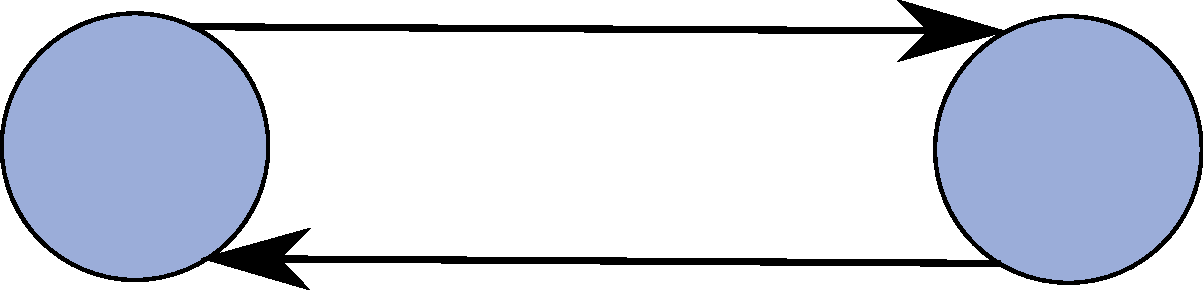
\includegraphics[width=1.78646in,height=0.38583in]{figs/mutual-cooperation-graph}
    \caption{A graph representing a situation of mutual cooperation. An arrow from A to B indicates
    that A can benefit B.}
    \label{mutual-cooperation-graph}
\end{figure}

In mutual relations like this, it is possible to apply causal
cooperation, although only if the interaction is
\href{https://en.wikipedia.org/wiki/Prisoner\%27s_dilemma\#The_iterated_prisoner.27s_dilemma}{repeated}
-- i.\,e. if my choice causally influences the other agent's
choice\footnote{Note that in causal cooperation, cooperative or
  uncooperative behavior
  \href{https://en.wikipedia.org/wiki/Reciprocity_(evolution)\#Indirect_reciprocity}{may}
  also causally affect bystanders and thus increase the probability that
  I can establish cooperation with them in the future.}, and then the
other agent's choice can causally influence my choice, etc.\footnote{Throughout
  this treatment, the graphs do not represent time and repetition. This
  could be done by taking the given static graphs and ``unfolding
  through time'', similar to how it is done when
  \href{https://en.wikipedia.org/wiki/Backpropagation_through_time}{applying
  backpropagation to recurrent neural networks}. The resulting graph
  may then resemble a
  \href{https://en.wikipedia.org/wiki/Unified_Modeling_Language\#Interaction_diagrams}{UML
  interaction diagram}.} For introductions to causal cooperation, see, e.\,g.
  Axelrod \citeyear{Axelrod2006-ci}, Trivers \citeyear{Trivers1971-rb}, Fehr and Gächter
  \citeyear{Fehr1999-pd}, Dawkins \citeyear{Dawkins1976-cd}, Taylor \citeyear{Taylor1987-wn}, and
  Buss \citeyear{Buss2015-kp}.

Superrational cooperation also works in the above scheme, although
repetition is not required. The
\href{https://en.wikipedia.org/wiki/Prisoner\%27s_dilemma}{prisoner's
dilemma}
(\href{http://plato.stanford.edu/entries/prisoner-dilemma/\#PDRepCauDecThe}{with
replicas} or twins) is one example of this sort of problem.

\subsubsection{Circular cooperative structures and indirect causal
reciprocity}\label{circular-cooperative-structures-and-indirect-causal-reciprocity}

In principle, it is possible to establish causal cooperation even in
cases where the two agents cannot directly benefit each other, provided
there is a repeated causal link from my own decision to the decision of
the agent who can benefit or hurt me, such that I can in some way reward
cooperation and punish defection. As an example, consider the following
variation of Hofstadter's donation game:

\begin{quote}
\textbf{Donation circle.} Omega has a list of 6 participants. The list
is
\href{https://en.wikipedia.org/wiki/Linked_list\#Circular_Linked_list}{circular},
meaning that every participant has a successor. Omega sends each
participant a letter, asking them to respond with single letter `C' (for
cooperate) or `D' (for defect) without communicating with each other. It
explains that by sending in `C', participants can increase their
successor's payoff by \$5. By sending in `D', they can increase their
own payoff by \$2. As usual, the participants are told that they are all
rational or that they use similar decision mechanisms. Every participant
only cares about the balance of her own bank account, and not about
Omega's or that of the other 6 participants. Upon receiving the letter,
should you cooperate or defect?

\textbf{Iterated donation circle.} Like the circular donation game, only
that the game is played many times (the exact number of times being
unknown to the players). In every round, each participant is informed of
their predecessor's past choices before deciding whether to send in `C'
or `D'.
\end{quote}

Circular structures such as these can be represented by graphs such as
the one in Figure \ref{circular-cooperation-graph}.

\begin{figure}[h!]
    \centering
    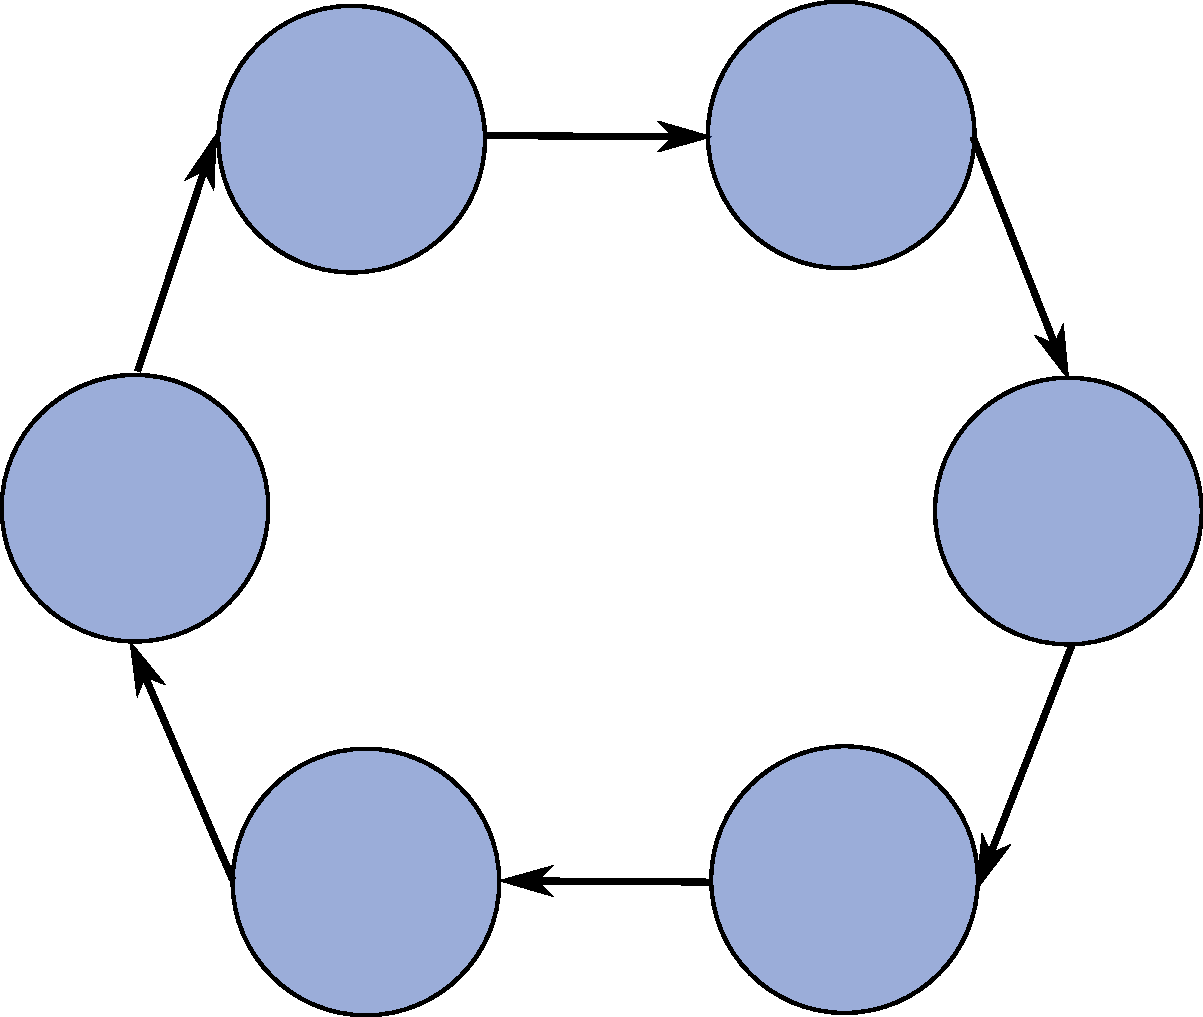
\includegraphics[width=1.68409in]{figs/circular-cooperation-graph}
    \caption{A circular cooperation graph
representing cooperation schemes of the sort used in the Donation
circle. Again, an arrow from A to B indicates that A can benefit B.}
    \label{circular-cooperation-graph}
\end{figure}

Because each of the agents can causally (through the other agents)
affect their predecessor, the iterated version of this problem could
still, in principle, motivate causal cooperation. For example, one
\href{https://en.wikipedia.org/wiki/Nash_equilibrium}{Nash
equilibrium} consists in everyone playing
\href{https://en.wikipedia.org/wiki/Tit_for_tat}{tit for tat}.
This Nash equilibrium is even
\href{https://en.wikipedia.org/wiki/Nash_equilibrium\#Stability}{stable},
in the sense that one player diverging from tit for tat with a very
small probability still leaves everyone else best off if they continue
to use tit for tat.

However, the same Nash equilibrium is also hard to achieve and unstable
in a different sense, as it requires all 6 participants to use the same
kind of strategy. Your response to your predecessor's cooperation is
mediated by multiple other agents. If only one of them does not
propagate your response correctly, the causal path from you to your
predecessor is disrupted, leaving neither of you with a causal
motivation to cooperate.

For superrationality-based considerations, on the other hand, neither
repetition nor the length of the causal path from one participant's
cooperation to her predecessor are relevant. Instead, superrational
cooperation only depends on the correlations between single pairs of agents.
Hence, while the significance of causal cooperation in the Donation
circle diminishes with every additional participant, the benefits from
superrational cooperation remain constant regardless of how many players
are involved.

\hypertarget{hierarchies-and-acyclic-graphs}{\subsubsection{Hierarchies
and acyclic graphs}\label{hierarchies-and-acyclic-graphs}}

In an extreme case, there would be no causal path whatsoever from one
participant's cooperation to that of his predecessor, making causal
cooperation lose its entire appeal to the rational agent. Superrational
cooperation, on the other hand, may still be applicable (cf.
Drescher \citeyear{Drescher2006-ky}; see
section \ref{gary-drescher-on-superrationality}).

Consider the following variant of the donation game:

\begin{quote}
\textbf{Donation ladder.} Once more, Omega has a long list of
participants, albeit a regular linear one this time. Omega sends all of
them a letter, asking them to respond with a single letter `C' (for
cooperate) or `D' (for defect) without communicating with each other. It
explains that by sending in `C', participants can increase their
successors' payoffs by \$5. The first person on the list cannot benefit
from the cooperative behavior of others, and the last participant's
choice has no effect on the others. Omega writes that each player can
increase their own payoff by \$2 if they defect. Participants do not
know their position on the list, and are once again told that they all
use similar decision algorithms. Every participant only cares about the
balance of their own bank account, and not about Omega's or that of the
other participants. Upon receiving the letter, should you cooperate or
defect?
\end{quote}

Figure \ref{donation-ladder} illustrates the donation
ladder.

\begin{figure}[h!]
    \centering
    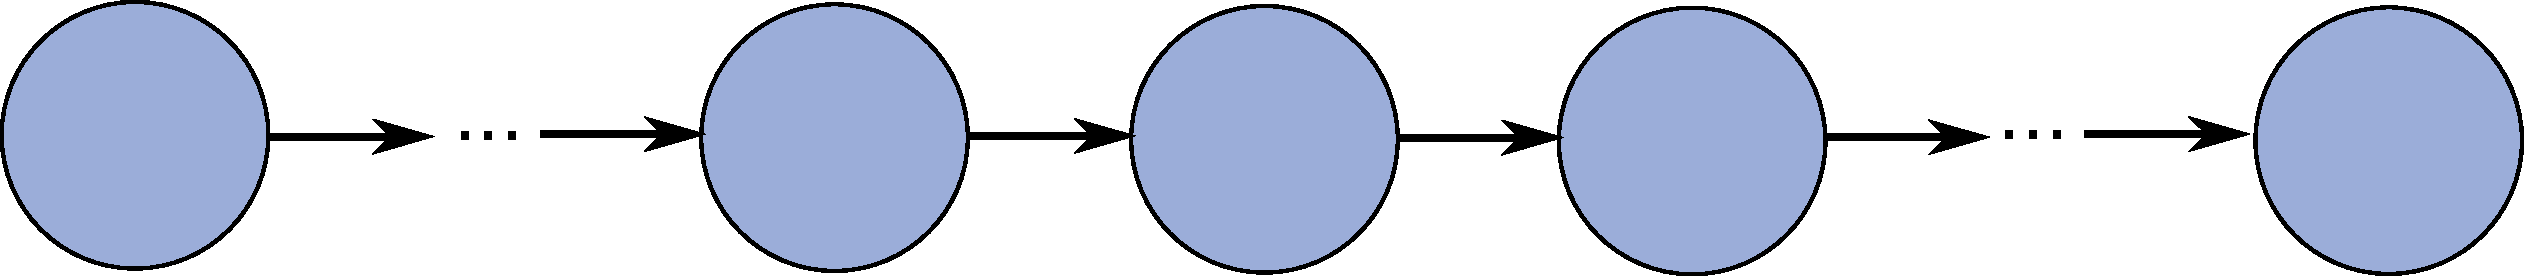
\includegraphics[width=5.19271in,height=0.49167in]{figs/donation-ladder}
    \caption{A linear cooperation graph (graph theoretically
speaking, a 1-ary tree) representing schemes of cooperation like that in
the donation ladder. An arrow from A to B indicates that A can benefit
B.}
    \label{donation-ladder}
\end{figure}

Again, the nodes represent participants and an arrow from A to B
indicates that A can bring causal benefits to B.

In such a cooperation scheme, causal cooperation cannot be established
even if the problem is iterated, whereas the superrationality mechanism
is just as reliable as in the other examples. Because the list is long,
I probably have a predecessor; if I cooperate, then my predecessor --
who is in a position similar to mine -- will probably make the same
choice. Cooperation thus informs me (or logically determines) that I am
likely to gain \$5, whereas defection only gives me \$2.

We can see this linear hierarchy of agents in practice among the
different versions of an agent at various points in time. For example, I
can causally affect the welfare of future versions of myself, but if I
only (or primarily) care about my present experiences, they can never
reward me in return. However, I could try to benefit future versions of
myself to make it more likely that past versions of me have behaved
nicely toward myself. More discussion with references to the literature
is given by \citet[section 7.3.4]{Drescher2006-ky}.

Linear cooperation hierarchies come with a twist, however. Consider the
following variant of the Linear hierarchical donation game:

\begin{quote}
\textbf{Donation ladder with known position.} Identical to the linear
hierarchical donation game, only that participants know their position
in the list when they make their decision.
\end{quote}

A participant in the middle of the list may wonder how his situation
differs from the regular donation ladder -- after all, his predecessor
on the list is in almost the same situation as he is. Assuming the
conditions for superrationality are satisfied, their decisions should
still correlate. Hence, if he cooperates, should we assume that his
predecessor is likely to do the same?

Not necessarily. The problem lies in the beginning of the list. The
first person -- let us call her No. 1 -- will have no predecessor and
thus no predecessor whose decision she could acausally influence, in
effect giving her no reason to cooperate. Given this, No. 1 should
defect (that is, unless she is already updateless; more on this below).

Unfortunately, this puts No. 2 in a similar position. Realizing that No.
1 will defect, there is nobody left to benefit \emph{him}. No. 3 will,
in turn, reason that No. 2 expects No. 1 to defect, which means that No.
2 will also defect, leading No. 3 to defect as well\ldots{} and so on,
propagating down the entire list. You may notice that this propagating
defection effect is analogous to the reason why
\href{https://en.wikipedia.org/wiki/Prisoner\%27s_dilemma\#The_iterated_prisoner.27s_dilemma}{standard
game theory recommends to defect in the iterated prisoner's dilemma when
the number of rounds is known}\footnote{Even in the iterated prisoner's
  dilemma, this answer -- supported by
  \href{https://en.wikipedia.org/wiki/Backward_induction}{backward
  induction} --
  \href{http://lesswrong.com/lw/to/the_truly_iterated_prisoners_dilemma/n23}{is
  often seen as unsatisfactory}. Other examples of paradoxes caused by
  backward induction are the
  \href{https://en.wikipedia.org/wiki/Chainstore_paradox}{chainstore
  paradox}, the
  \href{https://en.wikipedia.org/wiki/Traveler\%27s_dilemma}{traveler's
  dilemma}, the
  \href{https://en.wikipedia.org/wiki/Unexpected_hanging_paradox}{unexpected
  hanging paradox}, the
  \href{https://en.wikipedia.org/wiki/The_Bottle_Imp\#Bottle_Imp_paradox}{Bottle
  Imp paradox}, the
  \href{https://en.wikipedia.org/wiki/Centipede_game}{centipede
  game}, the
  \href{https://en.wikipedia.org/wiki/Interesting_number_paradox}{interesting
  number paradox}, the
  \href{https://en.wikipedia.org/wiki/Guess_2/3_of_the_average}{guess
  2/3 of the average game}. A good introduction is given by
  \href{http://www.cs.virginia.edu/~robins/The_Travelers_Dilemma.pdf}{Basu
  (2007)}. For further references, see Basu \citeyear{Basu1994-xk}.}.

Once more, we find that lack of knowledge is evidential power. For one,
if the participants did not know their positions, they would all
cooperate -- and thus be more successful. If everyone could precommit to
cooperation before learning about their position, they would do so.
Again, cooperation
\href{https://casparoesterheld.com/2016/11/21/thoughts-on-updatelessnes/}{can}
be maintained if all the agents are updateless in the first place (see
section
\ref{lack-of-knowledge-is-evidential-power-part-ii-taking-a-step-back}, cf.
\cite{Drescher2006-ky}, chapter 7.2.2). If all of this is not the
case, nothing can change the fact that at least No. 1
``\href{https://wiki.lesswrong.com/wiki/Rationality_is_systematized_winning}{wins}
by defecting once she knows her position on the list.

Secondly, thinking about the other agents' decisions can be dangerous.
No. 42 defects solely because he thinks about what the preceeding 41
participants decide. Knowing what the other agents think is thus harmful
for some not-yet-updateless decision theories. Hence, similar to how it
is wise to remain ignorant about your position in the list, many
decision theories would recommend not thinking about what the other
agents will do. If the players are human, then No. 1 may not be able to
refrain from realizing that he wins by defecting. Perhaps No. 2 cannot
refrain from realizing that No. 1's situation is different and his
decision therefore independent of hers. However, participants with
two-figure positions may be able to refrain and go with the reasoning
originally presented: whatever I choose, my predecessor will probably
choose the same, as his situation is similar to mine. If I just go ahead
without thinking about the ``chain of defection'' initiated by No. 1,
then people with similar numbers are probably going to do the same.

The linear structure can be generalized to non-linear hierarchical
cooperation schemes. Consider the following variant of the donation
game:

\begin{quote}
\textbf{Donation tree.} Omega has a long list of participants again. It
sends all of them a letter, asking them to respond with a single letter
`C' (for cooperate) or `D' (for defect) without communicating with each
other. Omega explains that by sending in `C', participants can increase
the payoff of at least 3 participants down the list by \$2 each. For
example, if the 4th participant chooses to cooperate, this benefits a
subset of the participants in positions 5, 6, etc. but not the previous
3 participants. The cooperation of the last few participants has little
to no effect. By sending in `D' participants can increase their own
payoff by \$5. Participants do not know their position on the list or
whom they could benefit. As usual, they are told that they all use
similar decision mechanisms. Every participant only cares about the
balance of their own bank account, and not about Omega's or the other
participants'. Upon receiving the letter, should a participant cooperate
or defect?
\end{quote}

In general, we can represent such hierarchical versions of the donation
game using
\href{https://en.wikipedia.org/wiki/Directed_acyclic_graph}{directed
acyclic graphs} like the one in Figure \ref{donation-DAG}.

\begin{figure}[h!]
    \centering
    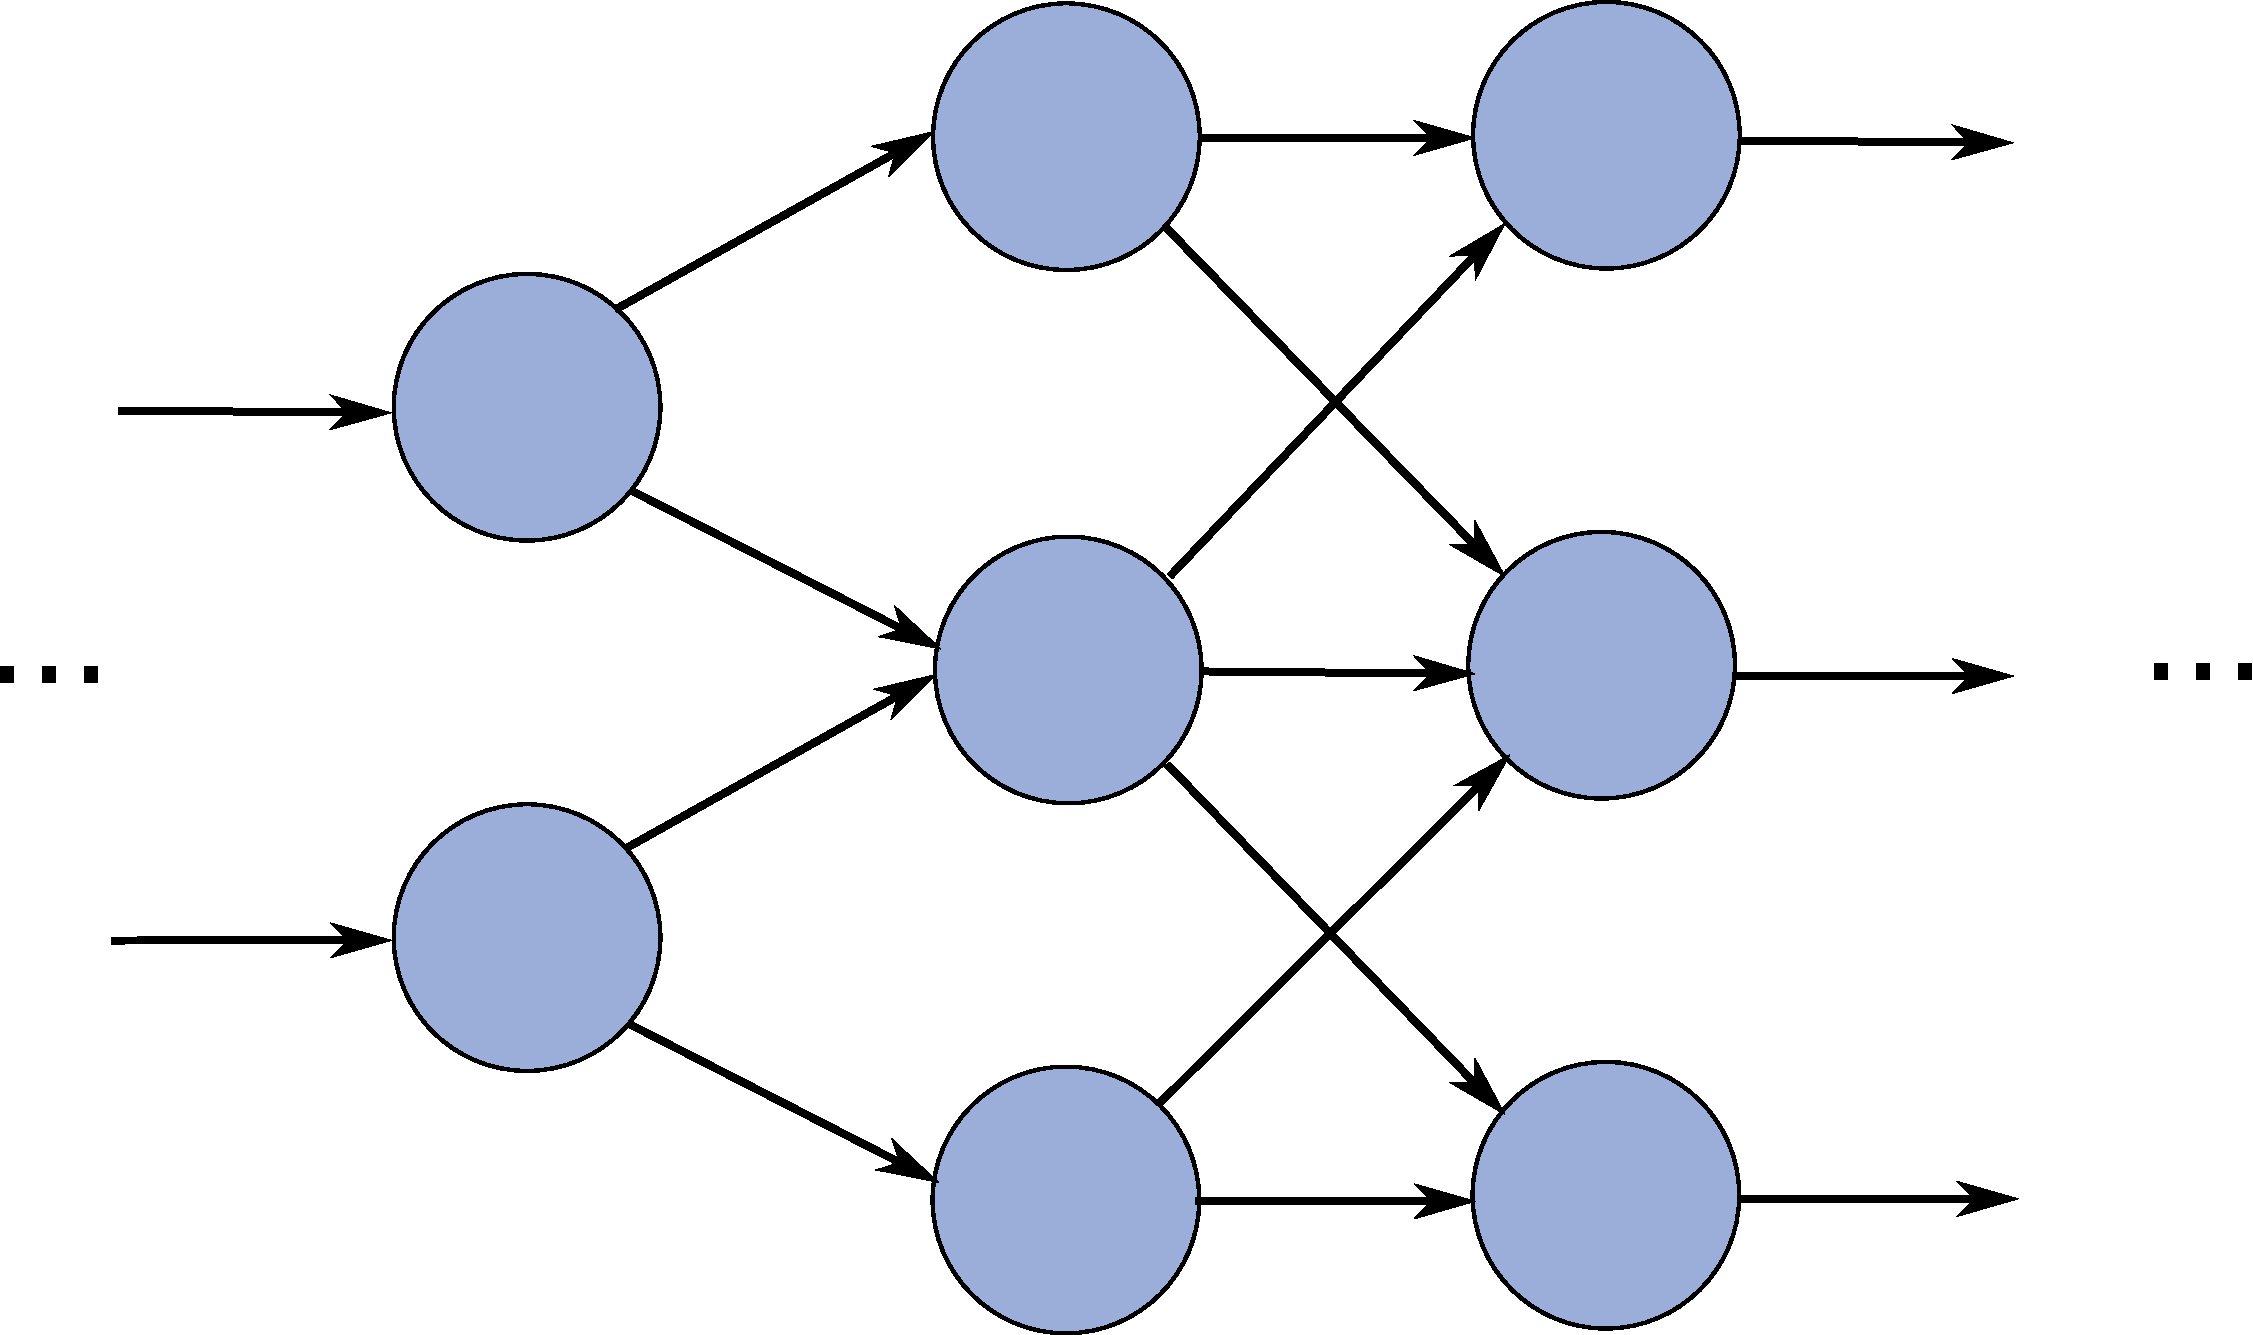
\includegraphics[width=3.98958in,height=2.05728in]{figs/donation-DAG}
    \caption{A directed acyclic graph representing the schemes of cooperation like that of the
    Hierarchical donation game.}
    \label{donation-DAG}
\end{figure}

If participants knew their respective positions in the list, the
considerations outlined for the Donation ladder with known position
would apply analogously.

In practice, such hierarchies may be hierarchies of power. Some agents
are ``lexically'' more powerful than others, such that cooperation can
only be beneficial in one direction -- the less powerful have no way of
helping the more powerful, while the powerful can help less powerful
ones much more cheaply. As a perhaps paradigmatic example, consider a
standard science-fiction scenario:

\begin{quote}
\textbf{Intergalactic relations.} The universe contains many
civilizations. Although they all followed similar evolutionary
trajectories, each civilization developed at different times on
different planets in different parts of the universe, and thus differ
drastically in their levels of sophistication. Most civilizations
eventually decided to conceal themselves to some extent, so no one knows
which of the civilizations is the most powerful. You are the leader of a
civilization, and one day, you encounter a comparably primitive
civilization for the first time. According to your advisors, it appears
that this other civilization has not even managed to harness the energy
of their local star, they still suffer from diseases that your
civilization's nano-devices could cure in an instant, and so forth. Your
advisors, citing the other civilization's apparently laughable defense
systems, recommend that you destroy them and use their resources to
further your own goals. Should you follow your advisors' recommendation?
\end{quote}

Once again, causal reasoning may suggest that you should. By now,
though, it should be clear that there are good reasons to ignore your
advisor's recommendation if you believe there is a sufficiently strong
correlation between your and the other civilizations.

Note that one reason for civilizations to conceal themselves might be to
induce a lack of knowledge about their relative positions within the
hierarchy. If we remain hidden, other civilizations will be more likely
to do the same, so neither we nor they would know who has the upper hand
in a potential confrontation. On the other hand, if all civilizations
loudly boasted their power, the most powerful civilization would realize
its dominance and consequently have no reason to be friendly to the
others -- absent precommitment, the use of updateless decision theory,
and the like.

Another example of such power hierarchies is that of simulations.
Simulators can causally influence the simulated in any way they want,
but the simulated can do little to causally affect the simulators (e.\,g.,
by
\href{https://foundational-research.org/how-the-simulation-argument-dampens-future-fanaticism\#Our_simulated_copies_can_still_impact_the_far_future_by_helping_our_simulators}{affecting
the outcomes of the simulation} or its computational demands). We will
discuss this more in section
\ref{simulations}.

The following example may be typical of the hierarchies in
multiverse-wide superrationality (MSR):

\begin{quote}
\textbf{Computable consequentialists.} Meet Luca, who believes that
consciousness cannot arise from
\href{https://en.wikipedia.org/wiki/Computability}{classical
computation} alone.\footnote{Two classes of hypotheses in this space
  are
  \href{https://en.wikipedia.org/wiki/Mind\%E2\%80\%93body_dualism\#Substance_dualism}{substance
  dualism} and the
  \href{https://en.wikipedia.org/wiki/Quantum_mind}{quantum
  mind}. Both have a few prominent proponents but are nonetheless
  fringe positions in philosophy of mind. I concur with the majority and
  am skeptical of both hypotheses.} He is also a consequentialist and
primarily cares about conscious experiences. Through the
\href{https://en.wikipedia.org/wiki/Mathematical_universe_hypothesis}{\emph{writings}
\emph{of Tegmark}}, Luca has come to believe that many computable
universes might exist in parallel to ours. However, since these
computable universes do not contain anything that he would call a
conscious experience, Luca does not care about what goes on inside them.
He does, however, enjoy thinking about their inhabitants as an
intellectual exercise, and this has led him to the conclusion that they
\emph{can} reason about Newcomb-like scenarios in a human-like way even
though they are insentient. After all, neither calculating conditional
probabilities nor operating on causal graphs requires sentience. Using
the supercomputer in his basement, Luca has also come up with a number
of predictions about the values held by consequentialists in the
computable universes -- let us call them the computable
consequentialists (CCs) -- a feat more difficult to achieve for
incomputable worlds. He has even discovered a number of ways to benefit
the CCs' values in our universe, all at a very low cost to his own
values. While Luca himself does not care about computable universes, he
sees no reason for the CCs not to care about worlds that are
computationally more powerful than their own. Given that the CCs cannot
do anything for Luca in their world, however, is it rational for Luca to
be friendly to the CCs' values?
\end{quote}

Again, Luca does indeed have a reason to do so. If he benefits the CCs,
other agents -- including ones whom Luca cannot benefit -- are more
likely to realize Luca's goals in other parts of the multiverse.

The ability to help can also come from knowing about the other agents.
Consider the following example:

\begin{quote}
\textbf{Simple-world ignorance.} Imagine a multiverse in which many
different sets of laws of physics are realized. Some of the universes
have very simple, parameterless, and easily understood basic laws, like
\href{https://en.wikipedia.org/wiki/Conway\%27s_Game_of_Life}{Conway's
Game of Life}. Others have far more complicated rules. The inhabitants
of the more complex universes may thus have more reason to believe in
the multiverse than the inhabitants of the simple universes. In the
complex universe, the multiverse hypothesis is attractive because it is
\href{http://lesswrong.com/lw/jp/occams_razor/}{simpler} than the
hypothesis that only their universe exists (cf.
\href{ftp://ftp.idsia.ch/pub/juergen/everything.pdf}{Schmidhuber
1997}). In the simple universe, on the other hand, the multiverse
hypothesis may be more complex than the hypothesis that only their
universe exists. Consequently, the inhabitants of the simple universes
may adopt superrationality but only apply it toward other inhabitants of
their universe. Let us assume that the values of the folks from the
simple universes differ significantly from those of the inhabitants of
the more complex universes. Should the inhabitants of the complex
universes help the values of those from the simple universes?
\end{quote}

In this scenario, as with the previous ones in this section, I think
that the superrationalists from the more complex universes have good
reason to help the superrationalists from the simpler universes, as this
makes it more probable that the former will receive help from other
agents, including ones that \emph{they} cannot help. For example, there
may be many value systems that \emph{they} (the inhabitants of the
complex universes) do not know about (for reasons other than the
Kolmogorov complexities of different multiverses).

I think this particular scenario may well be relevant in our multiverse.
More generally, some parts of the multiverse may contain different clues
about the existence of other superrational agents. For example, some
might live in parts of the universe from which it looks as though life
is much rarer than it actually is, whereas others may discover that they
are not alone as soon as they look through a telescope for the first
time. In addition, while a superrational agent may be able to use some
theory of physics to infer the existence of other agents, he or she may
be unable to infer the existence of some particular value system.

\hypertarget{only-helping-superrational-cooperators-helps-you-superrationally}{\subsubsection{Only
helping superrational cooperators helps you
superrationally}\label{only-helping-superrational-cooperators-helps-you-superrationally}}

Cooperation usually excludes agents who are known to be unable to
reciprocate. Yet as we learned from the Donation tree and Intergalactic
relations, superrationality does allow for cooperation with
non-reciprocating agents if helping them makes it more likely that other
agents help us.

There is, however, at least one limitation on the set of our
beneficiaries that comes without negative side-effects. We can exclude
from superrational cooperation all agents who do not cooperate
superrationally at all. After all, every superrational cooperator knows
that this exclusion will not affect her, and the exclusion appears to be
symmetrical among all superrational agents. That is, it makes it more
likely that other superrational cooperators make the same choice (rather
than incurring some other limitation that excludes us).

It seems risky to place any stronger limitation on the set of our
beneficiaries, since this would give us reason to fear exclusion by
other agents (cf. \cite{Drescher2006-ky}), as we have
seen in section
\ref{hierarchies-and-acyclic-graphs}. If we so much as try to look for rules of
exclusivity that benefit us at the expense of other superrational
agents, we have reason to believe that others will do so as well.

Of course, superrationality and correlation between decisions are not
binary properties, so neither is the limitation drawn above. For
example, two artificial intelligences explicitly based on the same
decision theory may correlate more than two (non-copied) humans, even if
both have some incentive to cooperate. The stronger the correlation
between us and some other agent, the more we will benefit
superrationally from helping them (cf.
\cite{Drescher2006-ky}). To illustrate this, consider a
one-shot prisoner's dilemma-like situation in which two very similar
agents can simultaneously decide whether to give the other one some
reward \(b_{\text{other}}\) or to walk away with a smaller reward
\(b_{u}\) for themselves. The cooperation graph looks like this:

\begin{figure*}[h!]
    \centering
    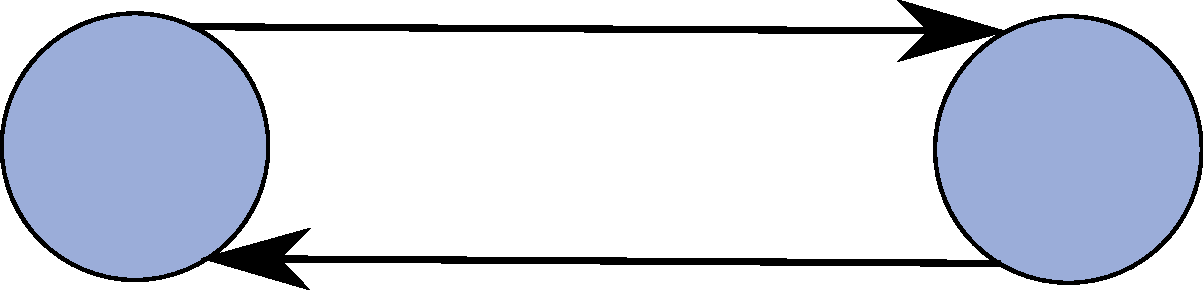
\includegraphics[width=1.78in]{figs/mutual-cooperation-graph}
\end{figure*}

Now, imagine the two agents are perfectly correlated, i.\,e. they always
make the same decision. If this is the case, both agents should
cooperate whenever
\begin{equation}
    b_{\text{other}} > b_{u}.
    \label{eq:condition_coop}
    % previously (*)
\end{equation}

Now consider a situation in which the correlation between the two agents
is weaker. Then, in EDT terms, they should cooperate if cooperation (C)
is higher in expected value than defection (D), i.\,e. if
$$
\mathbb{E}\lbrack C\rbrack > \mathbb{E}\lbrack D\rbrack.
$$

Using conditional probabilities, we can reformulate this as
$$
P(C\mid C) \cdot b_{\text{other}} > P(C\mid D) \cdot (b_{\text{other}} + b_{u}) + P(D\mid D) \cdot b_{u} =
P(C\mid D) \cdot b_{\text{other}} + b_{u},
$$
where, for example, \(P(C\mid C)\) is the probability that the other side
cooperates conditional on my cooperation. Solving for \(b_{\text{other}}\) yields
\begin{equation}
    b_{\text{other}} > \frac{b_{u}}{P(C\mid C) - P(C\mid D)},
    \label{eq:solve_p}
    % previously (**)
\end{equation}
where \(P(C\mid C) - P(C\mid D)\) can be interpreted as quantifying how much
more likely my cooperation makes the other's cooperation. Because there
is at least some correlation, the term is always greater than 0. If the
correlation is perfect, then \(P(C\mid C) = 1\) and \(P(C\mid D) = 0\), such
that we get Eq.~\eqref{eq:condition_coop} as a special case of Eq.~\eqref{eq:solve_p}. If the correlation is less
than perfect, then \(b_{a} > b_{s}\) may not be enough. For example, if
\(P(C\mid C) = 0.8 = P(D\mid D)\) (such that whatever one agent does, the other
agent is 80\% likely to do the same), then it must hold that
$$
b_{a} > \frac{b_{s}}{P(C\mid C) - P(C\mid D)} = \frac{b_{s}}{0.8 - 0.2} = \frac{5}{3}b_{s}.
$$
Thus, the threshold for cooperation increases as the correlation between
the two agents decreases.

If the cooperation graphs become more complicated, then so do
calculations like those above. Further research is needed to find out
whether the above result -- that benefitting agents with stronger
correlation is more important -- holds true more generally. One
interesting question is to what extent superrationalists would form
clusters based on correlation strength. This is especially relevant if
we believe the correlations to be especially strong among agents with
the same value system.

\hypertarget{cheating-signaling-and-half-heartedness}{\subsection{Cheating,
signaling, and
half-heartedness}\label{cheating-signaling-and-half-heartedness}}

Causal and superrational cooperation differ in another important
respect. In causal cooperation, the benefit of cooperative behavior
comes from how other agents will react to one's own cooperative
acts.\footnote{For references to the literature, see section
  \ref{schemes-of-causal-cooperation}.} To facilitate cooperation, each agent may
commit to reward cooperative and punish uncooperative behavior. In this
way, they can motivate each other to cooperate. But seeing as behavior
can only be rewarded or punished if it is observed at all, causal
cooperation often ends up focusing heavily on signalling. If you can
save costs by merely pretending (in a convincing way) to have
cooperated, then that is the rational thing to do from a causal
perspective. Conversely, if you can help someone without them knowing
about it, you have no causal reason to do so. There are many practical
examples of this, such as the tendency for governments to make a big
deal out of international agreements or cooperative acts, even if the
object-level gain is minor.

Since the mechanism of superrational cooperation is different from that
of regular causal cooperation, prioritization within it should be
different, too. Specifically, superrational cooperation is beneficial
not because others reciprocate one's cooperative acts, but because our
(cooperative) decisions correlate with those of others. This means that
we should sincerely attempt to maximize for benefits to other value
systems, because this correlates with others doing the same, which in
turn maximizes our own benefits.

We are used to thinking about cooperation in causal terms, i.\,e. about
how a certain cooperative act may in the end pay us back causally and in
this universe. If we think about superrational cooperation in this old
mindset, we may be tempted to propose measures that are critically
suboptimal from a superrational standpoint. For instance, one may adopt
a ``compartmentalized good will'', talking at length about cooperation
without actually trying to maximize for other agents' goal achievement,
or spend time thinking about how the others might cheat us.

However, all of these correlate with other superrational agents in the
multiverse wasting effort on these exact same things. With superrational
cooperation, only sincere attempts at improving other agents' value
systems correlate with the same behavior in others, and thus with the
optimal consequences. Hence, there is no way to ``game the system'' or
to get benefits without honestly paying for them.


\hypertarget{values}{\section{Values}\label{values}}
We extensively covered the mechanism of (multiverse-wide)
superrationality. However, in all thought experiments considered so far,
we knew what impact our actions would have on the fulfillment of the
other agents' preferences. For example, we know that the other
participants in the donation game or Platonia five would prefer to have
more money on their bank account. We also know that other civilizations
would prefer not to be destroyed in
\ref{hierarchies-and-acyclic-graphs} and would benefit from learning about our technologies. Such
knowledge has to be present or at least attainable in the future (cf.
section
\ref{cooperation-in-the-face-of-uncertainty-about-values}),
otherwise no side can benefit the others. This section gives an overview
of how we can find out what other agents in the multiverse care about,
as well as what aspects of their preferences we should focus on in the
first place.

\hypertarget{orthogonality-of-instrumental-rationality-and-values}{\subsection{Orthogonality
of instrumental rationality and
values}\label{orthogonality-of-instrumental-rationality-and-values}}

One objection to superrational cooperation might be based on a possible
convergence of terminal values, in which all agents with the correct
decision theory will converge toward the same values.
\href{https://en.wikipedia.org/wiki/Moral_realism}{Moral realism}
claims that there are facts in morality as real and true as those in
science. In addition, some moral realists believe that any rational
agent investigating morality will ultimately arrive at these moral
truths. Assuming that a large part of being rational involves using the
right decision theory, maybe all agents with the right decision theory
will independently come to adopt the ``correct'' moral system? If this
is the case, no cooperation among these agents would be necessary
(although some value systems may still require multiverse-wide
\ref{notes-on-superrational-coordination},
see section
\ref{notes-on-superrational-coordination}).

As a first counterargument, consider that knowledge of the
\emph{correct} decision is not necessary for superrational cooperation,
seeing as a
\href{https://casparoesterheld.com/a-comprehensive-list-of-decision-theories/}{number
of different decision theories} (e.\,g.,
\href{https://en.wikipedia.org/wiki/Evidential_decision_theory}{evidential},
\href{https://intelligence.org/files/TDT.pdf}{timeless} and
\href{https://wiki.lesswrong.com/wiki/Updateless_decision_theory}{updateless}
decision theory) imply superrationality. Secondly, we do not seem to
observe empirical evidence of such convergence. For example, Eliezer
Yudkowsky and Brian Tomasik agree that non-causal considerations are
important for decision theory, but
\href{https://wiki.lesswrong.com/wiki/Fun_theory}{Yudkowsky's
values} nevertheless differ significantly from
\href{http://reducing-suffering.org/\#Ethics}{Tomasik's}.

There are also principled reasons to be skeptical of value convergence
among agents with the same decision theory. Decision theories are about
\emph{instrumental rationality}, i.\,e. about making decisions aimed at
achieving goals, not at revising them\footnote{Apparently, some authors
  \href{https://en.wikipedia.org/wiki/Instrumental_and_value_rationality}{differentiate}
  between instrumental and ``value rationality''. I would probably
  disagree with the assumptions underlying the use of the term ``value
  rationality'' (see footnote \ref{non-cognitivism}).
  Nevertheless, I agree with the differentiation itself.}. That is at
least the case for decision theories as they are discussed today.
Consider the following variant of the donation game:

\begin{quote}
\textbf{Donation game for sadists.} Omega has selected 20 \emph{pure
sadists}, who draw pleasure only from torturing others and nothing else.
They all use similar decision making mechanisms when playing a donation
game (against correlated agents). Instead of being paid in dollar sums,
they are given individual hours to torture a slave as a reward.
\end{quote}

Assuming sufficient correlation between participants, the instrumentally
rational decision for each sadist is to cooperate such that the total
number of hours of torture increases relative to universal defection.
The moral choice, on the other hand, would be to defect in order to
reduce the number of hours in which anyone gets tortured. However,
decision theories (as currently discussed in the literature) do not take
moral considerations into account at all. They merely aim to fulfill the
goals, whatever they may be, of the agent using that decision theory.
Hence, when applied by a pure sadist, a given decision theory is meant
to help her spend more time torturing others.\footnote{In most human
  sadists, sadism is probably not the only goal or cause of happiness.
  Many sadists probably recognize their urges as morally wrong, yet are
  unable to control them to varying degrees. To these sadists, a
  decision theory may provide a nudge towards seeking professional help
  (at least if they cannot satisfy their sadistic preferences in morally
  nonproblematic ways).}

There could conceivably be some different kind of ``decision theory''
that does recommend taking morality into account (and not only
cooperation, see section \ref{real-altruism}) even if the agent using it is amoral or immoral. One
could, for instance, simply combine the correct decision theory with the
``correct'' moral view. Some people may consider such a decision theory
objectively correct. However, for an agent with immoral goals (like pure
sadism), it
\href{http://reducing-suffering.org/thoughts-on-postmodernism-and-its-intellectual-kin/\#Why_care_about_ethics}{would
be} instrumentally \emph{irrational} to adopt such a decision theory.
In any case, the existence of such a ``moral decision theory'' does not
contradict the existence of a decision theory in the classical,
instrumentally rational sense, so an amoral or immoral agent would still
be better off adopting a classical decision theory.

Thus, it would seem that an agent's values and their use of acausal
decision theories are orthogonal. This, in turn, suggests that agents
with a variety of value systems will adopt a decision theory similar to
our own, such that their decisions will correlate with ours.

Similar views regarding the relationship between
\href{http://lesswrong.com/lw/31/what_do_we_mean_by_rationality/}{instrumental
(and epistemic) rationality} and ethical values have been defended
under the term \emph{orthogonality thesis}
\parencite{Bostrom2014-pc,Bostrom2012-hj,Armstrong2013-xo}.

Our claim that decision theory and values are orthogonal in principle
does not imply that they never correlate in practice throughout the
multiverse. Indeed, in section
\ref{the-values-of-our-superrational-collaborators-in-the-multiverse} and its
companion papers, I will discuss various ways in which values and
decision algorithms could be expected to correlate. However, it seems
very unlikely to me that these correlations are so strong that they
significantly dampen the relevance of superrationality.

\hypertarget{necessary-preconditions}{\subsection{Necessary
preconditions}\label{necessary-preconditions}}

Before we start thinking about the values of agents in other parts of
the multiverse, we need to consider what kind of agents can join
multiverse-wide superrational cooperation (MSR) at all. In particular,
what sorts of values do they need to have, independent of whether or how
many such agents or value systems actually exist in the multiverse? We
already know that only helping superrational or correlated agents
benefits us (see section
\ref{only-helping-superrational-cooperators-helps-you-superrationally}).
However, the values of the superrationalists must also be open to the
opportunity of gains from compromise. If an agent's values imply that
she is better off without any trades, there is no point in helping her.
In order to more closely examine this precondition, we can break it into
five distinct criteria, all of which are necessary for a superrational
collaborator to reap the gains from compromise.

\begin{enumerate}
\def\labelenumi{\arabic{enumi}.}
\item
  Each collaborator must care to at least some extent about states of
  the world, as opposed to caring only about their own mental states or
  actions.
\item
  They must also care about consequences in areas of the multiverse
  where there may be other cooperators.
\item
  Other superrationalists must be able to infer and understand their
  values in sufficient detail. (To draw action-guiding conclusions from
  MSR, they themselves need to be able to infer the values of some other
  superrationalists or to influence future agents with this ability.)
\item
  Given this knowledge of their values, collaborators must have some
  power to behave nicely toward this value systems. (Again, if MSR is to
  be action-guiding to an agent, they in turn need to be able to benefit
  other values.)
\item
  Doing so produces gains from compromise. If everyone abides by an
  analogous cooperative strategy, everyone is better off than they would
  be without cooperation.
\end{enumerate}

If all these criteria are satisfied, superrational cooperation works. We
will discuss the first five criteria in the following sections. The
sixth is discussed in section
\ref{only-helping-superrational-cooperators-helps-you-superrationally}.

For some applications it may be fruitful to subdivide these criteria
further. Furthermore, additional criteria, such as
Bostrom's ``porosity'' \citeyear{Bostrom2014-gy}, may determine the
size of the gains from compromise. We could furthermore devise criteria
to assess the extent to which superrational cooperation affects one's
strategy. For instance, if all correlated agents have the same values
anyway, superrational cooperation does not affect our policy except for
cases of coordination (see section
\ref{notes-on-superrational-coordination}).

\hypertarget{consequentialism}{\subsubsection{Consequentialism}\label{consequentialism}}

Most people's ethical views are partly
\href{https://en.wikipedia.org/wiki/Deontological_ethics}{deontological}
(and sometimes
\href{https://en.wikipedia.org/wiki/Virtue_ethics}{virtue
ethical}). That is, they are not solely concerned about the state of
the world and the consequences of actions, but als about ``the actions
themselves'' (and, in case of virtue ethics, one's character). They
usually try to follow some set of rules prescribing what actions are
appropriate in which situations. For example, many people follow strict
rules against killing (though these usually do not apply under all
circumstances and the meaning of ``killing'' is rarely fully specified),
even when breaking these rules would lead to fewer deaths. This type of
ethical system forms a central part of many religious doctrines, with
notable examples such as the Christian ten commandments, the
\href{https://en.wikipedia.org/wiki/Ten_Commandments}{C}o\href{https://en.wikipedia.org/wiki/Ten_Commandments}{n}f\href{https://en.wikipedia.org/wiki/Ten_Commandments}{u}c\href{https://en.wikipedia.org/wiki/Ten_Commandments}{i}a\href{https://en.wikipedia.org/wiki/Ten_Commandments}{n}
\href{https://en.wikipedia.org/wiki/Filial_piety}{filial
piety}\href{https://en.wikipedia.org/wiki/Ten_Commandments}{,} and
Islamic sharia. In addition, most national laws contain countless rules
of this sort, many of which apply to more mundane domains like traffic
or taxes. Isaac Asimov's
\href{https://en.wikipedia.org/wiki/Three_Laws_of_Robotics}{three
laws of robotics} are yet another example of a deontological set of
rules.

The arguments for multiverse-wide superrational cooperation that I have
given appeal to the
\href{https://en.wikipedia.org/wiki/Consequentialism}{consequentialist}
aspects of one's values -- not because it requires us to push people off
bridges (as in the
\href{https://en.wikipedia.org/wiki/Trolley_problem\#The_fat_man}{Fat
man version of the Trolley problem}), but because its supporting
argument is fundamentally based on the consequences of different
actions. If we on Earth benefit other value systems, then this implies
that others elsewhere in the multiverse also benefit our value system,
which may produce better overall states of the multiverse overall via
\href{https://foundational-research.org/gains-from-trade-through-compromise/}{gains
from trade}. Hence, the value of superrational cooperation lies in its
positive consequences on the world (or other worlds). The ethical duties
of deontological ethical systems, on the other hand, usually concern the
more immediate consequences of our actions. Thus, in a scenario like the
Fat man version of the Trolley problem, most deontological would imply
that the direct act of killing the fat man violates our duties towards
him more than a failure to act violates our duty towards the five people
on the track.

In Bourget and Chalmers' survey of philosophers \parencite{Bourget2014-fm}, 23.6\%
of respondents characterized their values as consequentialist while
44.1\% identified as deontologists or virtue ethicists -- with the
remaining 32.3\% choosing ``other''. However, most people probably
espouse values that involve at least some consequentialist aspects (cf.
\cite{Muehlhauser2012-ib}). I doubt that many modern
consequentialists would be emotionally capable of murder or torture even
under circumstances where they could be confident that doing so would
yield the best consequences\footnote{In my personal experience,
  self-identified consequentialists actually tend to be more virtue
  ethical in their behavior than the average person.}. At the same time,
I doubt that many defendants of rule-based ethics see no appeal in
potentially reducing the amount of torture in the multiverse, even if
only in an indirect way. In fact, many deontological rules are motivated
or even defined by the consequences they produce. For example, murder is
defined as any act that intentionally and directly results in the death
of another person (although indirect ways of causing the same
consequence (e.\,g.,
\href{https://en.wikipedia.org/wiki/Omission_bias}{omissions})
are not seen as murder). Rules against theft are often defended on the
grounds that a society with such rules is preferable to one without,
even if the rules might occasionally prevent a genuinely altruistic bank
robbery. Some even
\href{http://briantomasik.com/interpreting-the-categorical-imperative/\#Categorical_imperative_as_decision_theory}{interpret}
Kant's
\href{https://en.wikipedia.org/wiki/Categorical_imperative}{categorical
imperative} (especially its first ``formulation'') as a heuristic based
on consequentially motivated decision-theoretical reasoning
\parencite{Parfit2011-xj,Hare1993-gi}. As Rawls \citeyear{Rawls1971-sq}
writes, ``deontological theories
are {[}not defined{]} as views that characterize the rightness of
institutions and acts independently from their consequences. All ethical
doctrines worth our attention take consequences into account in judging
rightness. One which did not would simply be irrational, crazy.''
Although most people refrain from the consequentialist choice in extreme
situations, they do, in fact, often endorse it. For example, in
Bourget and Chalmers' survey \citeyear{Bourget2014-fm}, 68.2\% of the respondents
chose to pull the switch in the original
\href{https://en.wikipedia.org/wiki/Trolley_problem}{trolley
problem}, and only 7.6\% did not (with the remaining 24.2\% choosing
``other''). Pulling the switch
\href{https://en.wikipedia.org/wiki/Trolley_problem\#Psychology}{is
similarly popular} among the general population. This suggests that
people sometimes agree with consequentialist reasoning even if other,
exclusively deontological or virtue ethical considerations can overrule
it.

Beyond consequences for things like the number of deaths, individual
welfare, and fairness, people sometimes also care about the abidance by
deontological rules in a consequentialist way. For example, most people
not only avoid killing others themselves, but also care about preventing
murders in general; many who personally avoid lying also strongly
dislike it when others lie; and so forth. These kinds of
consequentialism, which are rarely considered in the literature on moral
philosophy, qualify for superrational consideration just as much as,
say,
\href{https://en.wikipedia.org/wiki/Utilitarianism}{utilitarianism}.
We will revisit this topic of caring about the deontologically ethical
behavior of others in section
\ref{human-far-values}, in
which we review studies indicating that many people have values of this
sort.

\hypertarget{caring-about-the-multiverse}{\subsubsection{Caring about
the multiverse}\label{caring-about-the-multiverse}}

Presumably, some agents with significant consequentialist aspects to
their values will almost exclusively care about their own part of the
multiverse, if only based on
\href{https://en.wikipedia.org/wiki/Ethical_egoism}{egoism} or
\href{https://wiki.lesswrong.com/wiki/Absurdity_heuristic}{absurdity
heuristics}\footnote{One may argue that absurdity heuristics are a part
  of someone's
  \href{https://en.wikipedia.org/wiki/Epistemology}{epistemology}.
  That is, the ``absurdity'' of the Everett interpretation is used as a
  reason to give it low probability as a theory of physics. However, it
  \href{http://reducing-suffering.org/why-does-physics-exist/\#My_new_understanding}{is
  not clear} whether there is a clear-cut, operational difference
  between belief and preference if the belief does not make a testable
  prediction.}. It is thus very difficult or impossible to benefit them
in other parts of the multiverse, in turn preventing cooperation.

Although there is very little discussion about the moral relevance of
other parts of the multiverse, the moral relevance of distance is
frequently discussed in moral philosophy (see, e.\,g.,
\citet{Brock2013-cv}. Note that while distance is
usually understood to be spatial, other kinds of distance (e.\,g.,
\href{https://sentience-politics.org/philosophy/the-importance-of-the-future/}{temporal}
\parencite{Beckstead2013-lv} or social) play similar roles
in ethical judgment.

While the debate in moral philosophy appears ambiguous, people's actions
speak more clearly. Most people from high-income countries would save a
child from drowning in a nearby pond, but donate
\href{http://nccs.urban.org/nccs/statistics/charitable-giving-in-america-some-facts-and-figures.cfm}{only
relatively small} amounts to charity
\parencite{Singer1972-uk}. Insofar as they do give to
charity, they usually prefer local causes even though helping in
low-income countries
\href{http://www.givewell.org/giving101/Your-dollar-goes-further-overseas}{is}
more cost-effective. From this, we can safely infer that most people are
altruistic to some extent, but seem to care more about near events
rather than distant ones.

One may suspect that an agent's ignorance about other parts of the
multiverse would yield similar conclusions as a lack of interest. After
all, if someone does not know about our part of the multiverse, they
cannot help us. However, we must not forget that superrational
cooperation need not be based on mutuality (see section
\ref{no-reciprocity-needed-whom-to-treat-beneficially}). Even if someone
cannot help us, we can still help them to make it more likely that we
ourselves receive help from agents whom \emph{we} cannot help.

\subsubsection{Knowable values}\label{knowable-values}

In order to maximize for some given utility function, we or future
superrationalists (see section
\ref{cooperation-in-the-face-of-uncertainty-about-values}) need a
sufficiently detailed model of the utility function itself. In section
\ref{the-values-of-our-superrational-collaborators-in-the-multiverse}, we will discuss how the
evolutionary psychology of morality and related disciplines can be used to assess the values of
superrational cooperators in the multiverse. There are at least some ways of making very educated
guesses, although we cannot expect to arrive at a detailed and precise description of the values of
all evolved civilizations and their descendants. However, perfect knowledge is not necessary for our
purposes. Indeed, most people cannot even describe their own values in detail (see footnote
\ref{we-do-not-know-our-utility-function}). Yet despite this, humans are perfectly capable of
helping one another achieve their goals. Thus, the question is neither whether we can gain relevant
knowledge about the values of other agents in the multiverse at all, nor whether we can have a full
map of extraterrestrial morality, but whether the information we can gather about other
civilizations can be \emph{sufficiently} accurate to yield a usable model.

\hypertarget{fragility-of-value}{\paragraph{Fragility of
value}\label{fragility-of-value}}

Eliezer Yudkowsky \citeyear{Yudkowsky2015-tz} argues that human
values are not just complex (cf. section
\ref{organizing-human-values});
they are also fragile, in the sense that even minor errors in a
non-human agent's picture of them can completely derail that agent's
efforts to optimize for them. According to Yudkowsky, ``Any Future not
shaped by a goal system with detailed reliable inheritance from human
morals and metamorals, will contain almost nothing of worth.'' Perhaps
more generally, we could say that any resource expenditure will generate
next to no value for an intelligent evolved being X unless that resource
expenditure is shaped by a detailed inheritance of X's morals and
metamorals. Yudkowsky gives boredom as an example of a small but
indispensable part of human values:

\begin{quote}
``Consider the
\href{http://lesswrong.com/lw/xr/in_praise_of_boredom/}{incredibly
important human value of `boredom'} -- our desire not to do `the same
thing' over and over and over again. You can imagine a mind that
contained almost the whole specification of human value, almost all the
morals and metamorals, but left out just this one thing and so it spent
until the end of time, and until the farthest reaches of its light cone,
replaying a single highly optimized experience, over and over and over
again.''
\end{quote}

Presumably, many other seemingly insignificant aspects of human values
are of similar importance as boredom. One would need to get all of these
aspects just right in order to benefit human values. This suggests that
it will be difficult to benefit many evolved value systems, due to the
large amount of detailed knowledge it would require and the difficulty
of gathering that knowledge.

There are various points to discuss in this context. For one, the
fragility thesis is rather vague; it does not say \emph{how} fragile our
values are, or \emph{how} accurate and reliable the inheritance must be.
This is not to say that the fragility thesis makes no testable claim at
all. Yudkowsky formulated it with the
\href{http://lesswrong.com/lw/llr/superintelligence_20_the_valueloading_problem/}{value
loading problem of artificial intelligence} in mind. Since AIs can be
programmed to pursue any goal (cf. section
\ref{orthogonality-of-instrumental-rationality-and-values}), the space of possible
values with which an AI could end up is vast, and the target goal
systems occupy only a small fraction of this space. The fragility
hypothesis can be interpreted as one elaboration on just how small this
part of value space is, and how catastrophic it would be (from the
perspective of that value system) to miss it by even a small margin. In
other words: even if we take care to represent all of the most central
aspects of our values (e.\,g., ``increase the welfare of sentient beings''
or ``reduce inequality'') in the goal system of an AI, the outcome may
still be as bad as an entirely random one if we omit seemingly
peripheral values such as boredom.

Although I agree with the fragility thesis as a descriptive (rather than
normative) statement about human values, I do not think human values are
quite as fragile as Yudkowsky writes. Specifically, I think the outcomes
brought about by AIs with two different goal systems can differ
enormously in their overall worth even if both miss important aspects of
human values. For example, Yudkowsky's hypothetical world full of
repetitive happiness may be boring, but it is still much better than a
world full of suffering, unethical behavior, etc. and nothing of worth
to compensate. But perhaps this judgment is influenced by my own values
(which are mostly about ensuring the welfare of sentient beings with a
strong priority for preventing their
\href{https://foundational-research.org/the-case-for-suffering-focused-ethics/}{suffering}),
to the point where it would not generalize to how other humans, or other
evolved agents in general, would view the situation. Transferred to our
variant of the fragility thesis, this nevertheless suggests that even if
we miss significant parts of the values of other superrational
cooperators, taking their values into account may still make a big
difference to them.

More importantly, AI value loading differs significantly from our
attempt to benefit agents in other parts of the multiverse. The main
problem of AI value loading is getting the AI to care intrinsically
about human values. MSR, on the other hand, already gives us the sincere
(instrumental) goal of helping other agents, which the AI lacks. If
anything, we lack \emph{knowledge} of the others' values, whereas AIs
\href{http://lesswrong.com/lw/igf/the_genie_knows_but_doesnt_care/}{may}
still not care about them even with perfect knowledge of their values.

Another crucial difference between these two contexts is that in AI
value loading, we usually want the AI to hold the values of one
particular species or group of people. In contrast, when cooperating
superrationally, it is sufficient to know that we benefit many other
superrational agents. We do not need to know whether we benefit some
\emph{particular} species. The extent to which this makes our job easier
depends on how evolved value systems are distributed over value space.
Perhaps they form a few (or many) very small clusters, as depicted in
Figure \ref{map-of-value-space-with-clusters}.
(Needless to say, Figure
\ref{map-of-value-space-with-clusters} is not meant to
be an accurate map of value space. The placements on the map have no
factual basis.)

\begin{figure}[h!]
    \centering
    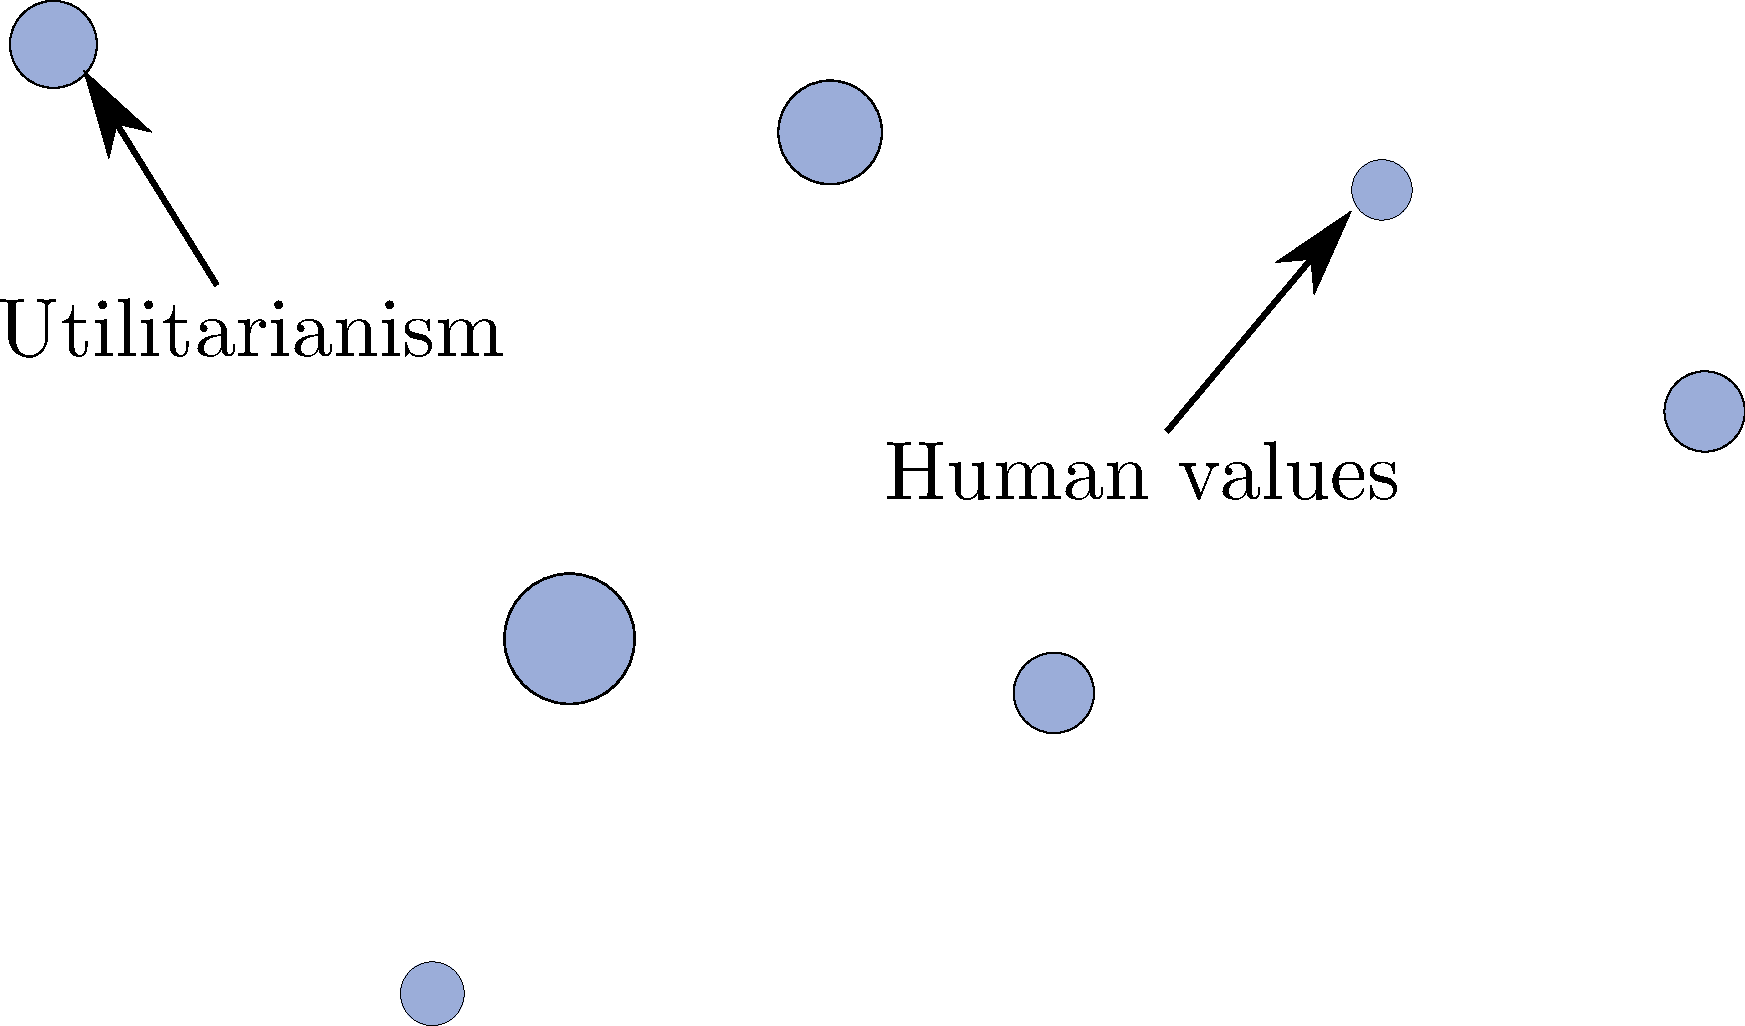
\includegraphics[width=3.21875in,height=2.54167in]{figs/map-of-value-space-with-clusters}
    \caption{A map of a part of value
space under the assumption of there being distinct clusters with a lot
of empty space in between.}
    \label{map-of-value-space-with-clusters}
\end{figure}

Every blue point on the map is some value system held by a significant
number of agents. The white areas of the map contain value systems that
do not have a significant following, such as
\href{https://wiki.lesswrong.com/wiki/Paperclip_maximizer}{paperclip
maximization}. If our map really did represent value space and each
individual value system is fragile, then it is difficult to benefit
other value systems, because if we miss the targets only by a bit, we
end up with a value set that nobody cares about. However, it could also
be that the values of different evolved agents occupy some compact part
of value space, as depicted in Figure
\ref{map-of-value-space-compact}.

\begin{figure}[h!]
    \centering
    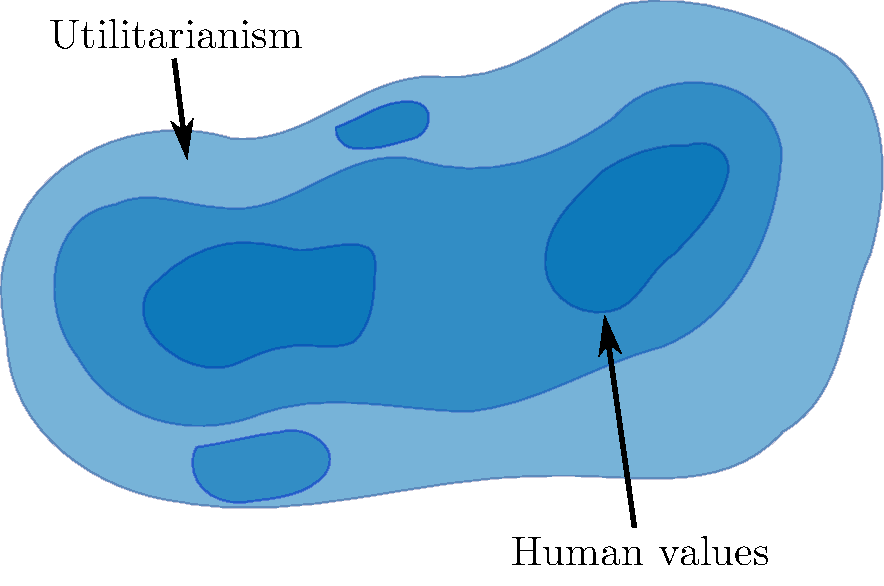
\includegraphics[width=3.26772in]{figs/map-of-value-space-compact}
    \caption{A map of a part of value space under the assumption that extant values occupy a
    relatively compact part of value space.}
    \label{map-of-value-space-compact}
\end{figure}

In this map, darker areas represent value systems with many agents and
lighter areas indicate value systems with fewer agents. If value space
looks more like this map than our previous one, then it is easier to
make ``guesses into value space'' to help superrational collaborators.
As long as one is roughly aiming at the right part of value space, small
errors just mean that one benefits slightly different superrationalists
than intended.

Only a few maps of humanity's value space have been created, the
best-known of which is probably the
\href{https://en.wikipedia.org/wiki/Inglehart\%E2\%80\%93Welzel_cultural_map_of_the_world}{Inglehart-Welzel
cultural map of the world}. I would nonetheless wager some guesses as
to how more fine-grained maps of values would look like: on any
individual planet, there are clusters formed by major religions,
nations, political camps, and other cultural groups. For example, there
are many people who hold many of the moral views of the Quran and many
who hold many of the moral views of the Bible, but presumably much fewer
who defend a mix of the two. Nonetheless, the space between the clusters
is not completely ``uninhabited''. Furthermore, the existence of these
clusters seems to be partly arbitrary, a mere result of the way that
different ideas were packaged together historically.
\href{https://en.wikipedia.org/wiki/Path_dependence}{If things had
gone slightly differently}, as they doubtlessly do in other parts of
the multiverse, the authors of the Bible may have written that it is
mandatory to fast during the month of Ramadan, thus filling a spot in
value space with life that is only sparsely inhabited on Earth. If the
multiverse is large enough, all these possible variations of values are
realized somewhere and probably no less common than the two religion
clusters on Earth.

One last difference between the way we extract values from other
superrational cooperators and the way AIs might receive their values
from humans is, of course, that the former involves no direct contact.
Section \ref{the-values-of-our-superrational-collaborators-in-the-multiverse} will address ways of
circumventing this problem in order to identify the values of agents elsewhere in the multiverse.

\subsubsection{The ability to help
others}\label{the-ability-to-help-others}

In some cases, it will not be in our power to help other value systems
\emph{at all}. Since any will to cooperate with these agents cannot
possibly be action-guiding, we do not have to help them. Other agents in
the universe may have other resources available to them and thus choose
to behave in a friendly way toward these values. If, on the other hand,
agents know that nobody else can help them to achieve their goals,
multiverse-wide superrational cooperation (in particular, any version of
it in which they just give resources away) becomes less attractive to
them.

One example of a value system that we cannot help is the following
version of
\href{https://en.wikipedia.org/wiki/Speciesism}{speciesism} (that
may or may not be a
\href{https://en.wikipedia.org/wiki/Straw_man}{straw man}):

\begin{quote}
\textbf{The Namuh-centrists.} One day, scientists inform you about a
highly intelligent species of extraterrestrials known as ``Namuhs''.
Like us, the Namuhs have built a flourishing civilization with art,
trade, science, language, humor, philosophy (including advanced decision
theory research), and so on. However, the Namuhs do not live in our
universe, but in a distant part of the multiverse, completely
inaccessible to us. In fact, they could not even exist in our part of
the multiverse, as their bodies require slightly different laws of
physics to function. Knowing about superrational cooperation, you hasten
to ask whether they have thought about problems analogous to
\href{https://en.wikipedia.org/wiki/Newcomb\%27s_paradox}{Newcomb's
problem} and the donation games between similar agents. A trustworthy
scientist explains that their minds are indeed prone to thinking about
such topics -- much more so than those of humans, in fact!
Understandably thrilled, you ask what values the Namuhs have, and
specifically what values are held by those who have thought about
acausal cooperation. The scientist then informs you that all Namuhs are
very narrowly focused on their own species. They are Namuh-centrists who
do not care one bit about anything that does not involve fellow Namuhs.
For example, they shrug at the thought of non-Namuh
\href{https://foundational-research.org/the-case-for-suffering-focused-ethics/}{suffering},
the flourishing of non-Namuh civilizations, or non-Namuh well-being. In
fact, they are so strict that they do not even care about simulated
Namuhs or other approximations.
\end{quote}

Learning about their values, you may be disappointed. There is nothing
that you can do to help them and it is therefore irrelevant whether they
use a decision theory similar to yours or not.

I should point out that the speciesism endorsed by the imaginary Namuhs
is very rigid and more narrow than most other views that we would
usually classify as speciesist. Far from caring only about their own
species, most people seem to care about the welfare of non-human animals
to at least some degree, usually while privileging some species (like
cats and dogs) over others (like pigs and cows). Such views classify as
speciesist, but nevertheless allow for superrational cooperation. Other
views do not value humans over other animals for their species
membership per se, but instead privilege other characteristics that
(allegedly) only humans (and sometimes a few other species) possess. A
\href{https://en.wikipedia.org/wiki/Animal_consciousness\#Philosophical_background}{common
variant} of this holds\footnote{Note that some authors are skeptical to
  there being any fact of the matter in questioning whether some being
  is conscious or not. Instead, they view terms like ``consciousness''
  and ``sentience'' as definitional categories or expressions of
  particular values. See, e.\,g., Dennett \citeyear{Dennett1991-es}
  and Brian Tomasik's
  \href{http://reducing-suffering.org/dissolving-confusion-about-consciousness/}{Dissolving
  Confusion about Consciousness}.} that only members of very few
species are conscious. Humans are one of them, but, according to such
views, they otherwise do not deserve any special moral status. Given the
implications of this view, proponents are sometimes (and often
incorrectly) branded as speciesist. If the Namuhs were to hold such a
view, and humans (or other earthly species) meet their criteria for
consciousness, then our decisions \emph{can} be beneficial or
detrimental to the Namuhs' preference fulfillment. A similar reasoning
applies to the
\href{https://en.wikipedia.org/wiki/Animal_consciousness\#Language}{possession
of language}, \href{https://en.wikipedia.org/wiki/Free_will}{free
will},
\href{https://en.wikipedia.org/wiki/Animal_consciousness\#Mirror_test}{the
ability to pass the mirror test} or other (potentially) strict but
non-speciesist restrictions to one's set of morally relevant agents.

There are other reasons why we might be (practically) unable to help
other agents. For example, helping an agent could require some set of
specialized abilities that they themselves developed based on their
value systems. Consider the following example:

\begin{quote}
\textbf{The Advanced math maximizers.} One day, you learn that out there
in the multiverse, there are civilizations made up entirely of
mathematicians whose primary concern is maximizing mathematical
knowledge. They don't care about the number of established truths or
proofs per se, but rather value pieces of knowledge based on their
novelty or interestingness, possibly resembling the way earthly
mathematicians often prioritize their research. For instance, the
mathematicians place a very high value on a proof or disproof of the
\href{https://en.wikipedia.org/wiki/Riemann_hypothesis}{Riemann
hypothesis}, whereas mundane factoids like the three-billionth digit of
\(\pi\) have very little value in comparison. Moreover, once a fact
becomes known to at least one of the mathematicians, reproducing that
same piece of information elsewhere in the multiverse creates no
additional value for them. (We assume that the universe is finite --
otherwise every piece of knowledge may be known to some
\href{https://en.wikipedia.org/wiki/Boltzmann_brain}{Boltzmann
brain}.) While they are not particularly skilled at anything else,
their strong intrinsic motivation and dedication has made them into
truly excellent mathematicians, unrivalled by anyone across the
multiverse.
\end{quote}

It is not easy to benefit the advanced math maximizers. We do not know
what knowledge they already possess, and given their level of skill, we
should assume that they will come up with most interesting pieces of
mathematical knowledge that we could devise on our own. The math
maximizers are thus so capable of maximizing their own utility function
that there is little we could do to assist them (cf. section
\ref{gains-through-specialization-and-comparative-advantages}).

\hypertarget{zero-sum-and-below-zero-sum-tradeoffs-on-resources}{\subsubsection{Zero-sum
and ``below-zero-sum'' tradeoffs on
resources}\label{zero-sum-and-below-zero-sum-tradeoffs-on-resources}}

Not all interactions between agents allow for cooperation. Specifically,
there is no way or reason to cooperate in
\href{https://en.wikipedia.org/wiki/Zero-sum_game}{zero-sum}
\href{https://en.wikipedia.org/wiki/Zero-sum_game}{g}a\href{https://en.wikipedia.org/wiki/Zero-sum_game}{m}e\href{https://en.wikipedia.org/wiki/Zero-sum_game}{s},
i.\,e. ones in which the overall payoff is always the same. Consider the
following example:

\begin{quote}
\textbf{The Maximizer Monarchs.} Imagine a multiverse consisting of two
universes. One is ruled by a queen whose only drive it is to create as
many paperclips as possible. The other universe is ruled by a king who
only cares about producing as many staples as possible. Each
stationery-maximizing monarch knows that the other exists and that they
both use the same decision algorithms. They each have one hundred tons
of steel at their disposal. What should they do with it?
\end{quote}

Assuming that staples (specifically the kind of staples that the queen
cares about) cannot be built out of paperclips or vice versa, this
interaction is zero-sum. Every bit of material that one of them uses for
the benefit of the other is an equivalent loss to themselves\footnote{If
  we normalize their utility function, both assign the same utility to a
  situation in which all the multiverse's metal is transformed into
  their favorite office supply. This also means that they assign the
  same utility to any other other fixed amount of metal being
  transformed into paperclips.}. Thus, no form of cooperation between
the two is beneficial.

As the reader may suspect, zero-sum interactions are rare. We should
expect that any given resource is better suited to achieving one goal
than another and so trade can arise from allocating resources based on
what value systems benefit most from them. Analogously, value systems
care more about certain situations than others. Furthermore, whereas it
may not be possible to combine a paperclip and a staple, many goals are
compatible with each other. For example, a society's citizens can at the
same time be happy and virtuous.

\hypertarget{gains-through-specialization-and-comparative-advantages}{\paragraph{Gains
through specialization and comparative
advantages}\label{gains-through-specialization-and-comparative-advantages}}

At times, trying to achieve multiple goals at once is not just pointless
-- it can actually be worse than having each agent focus on one,
typically their own, goal. To see how, let us revisit The Maximizer
Monarchs of the previous section:

\begin{quote}
\textbf{The Ever-improving Maximizer Monarchs.} Like The Maximizer
Monarchs, but this time, the efficiency at which each agent can produce
paperclips or staples grows monotonically with the produced quantity.
Again, each monarch wields one hundred tons of steel.
\end{quote}

Without delving into mathematical details, it is best (in terms of
overall number of paperclips/staples produced) if each of the two
specializes in one kind of stationery. In particular, there are no gains
from compromise over each monarch maximizing only for their own goals.

There may also be
\href{https://en.wikipedia.org/wiki/Comparative_advantage}{comparative
advantages} from the outset. Based on their respective motivation and
prior experience, the queen may already excel at producing paperclips,
while the king may be better at producing staples. Another important
source of comparative advantages is unequal knowledge about different
value systems. For example, if the queen does not know exactly what the
king cares about, then she will be worse at benefitting him. Similarly,
our knowledge of what other humans care about is much more precise than
our knowledge of what agents elsewhere in the multiverse care about.

The fact that specialization and division of labor play such a crucial
role in the economy suggests that superrationalists will also tend to
focus on a single goal rather than maximizing for multiple things at
once. However, I think that this will not be the case, at least in our
present situation. The primary reason is that the instrumental goals of
agents with different moral values are often the same. For example, no
matter the direction into which we would like to drive society, we will
try to acquire money and political influence. These resources are often
generic, such that when they are acquired with one goal in mind, they
can also be employed in pursuit of another. As an example, consider how
Donald Trump maximized his personal monetary wealth for a long time, yet
his resulting fame and money nevertheless enabled him to become
president of the US, which in turn allows him to achieve all kinds of
goals. The fact that instrumental goals tend to converge suggests that
superrationalists in the multiverse rarely have a strong comparative
advantage at achieving their own goals.

If comparative advantages are not strongly aligned with goals,
specialization can produce gains as well. For example, imagine a number
of superrational agents, each of whom would like to maximize many
different things separately, e.\,g., knowledge, fun, happiness and
technology. Here, a no-compromise outcome -- i.\,e. one wherein each agent
only maximizes their utility function in their own universe -- might be
worse than a potential division of labor with one agent focusing on
generating knowledge, another one focusing on fun, and so forth.

\hypertarget{what-values}{\subsection{What values?}\label{what-values}}

To help other agents, one at some point needs to have some workable
model of their preferences. In general, it is difficult to extract
preferences from a given agent
\href{http://lesswrong.com/lw/h45/we_dont_have_a_utility_function/}{if}
the agent is not
\href{https://en.wikipedia.org/wiki/Von_Neumann\%E2\%80\%93Morgenstern_utility_theorem}{von
Neumann-Morgenstern (vNM) rational} and cannot state her goal
explicitly. Humans surely
\href{https://en.wikipedia.org/wiki/Cognitive_bias}{are not}
vNM-rational. Additionally, moral judgments are usually seen as being
inaccessible to us in their complete form (see footnote
\ref{we-do-not-know-our-utility-function}) and as emerging from the whole
brain rather than exclusively from, say, the anterior cingulate cortex.
This makes sense from an evolutionary point of view. Preferences are
tools for increasing the fitness of an organism, and there is no reason
to assume that such tools would be any more open to scrutiny by the
organism than, say, the detailed inner workings of the digestive system.
In addition, while most organisms have rudimentary mechanisms for
avoiding harm and seeking food and reproduction, holding grudges -- i.\,e.
a preference for retaliation -- is only adaptive in non-solitary
organisms with sufficiently good memory and recognition to correctly
identify transgressors. In the evolutionary process, different values
thus evolve separately and are unlikely to form a coherent whole (cf.
\cite{Dennett1991-es,Kurzban2012-vt}).

Thus, even if we had a complete model of our superrational
collaborators, it would nevertheless be difficult to extract clear-cut
values from them. In the absence of such exact models, it makes little
sense to for us to discuss the technical details of relevant preference
extraction algorithms\footnote{\label{fn:prefs} Examples are described in Hansson and Grüne-Yanoff
\citeyear{Hansson2012-um}, Varian \citeyear{Varian2006-vw}, Neumann and Morgenstern
\citeyear{Von_Neumann1953-mc}, Ng and Russel \citeyear{Ng2000-xw}, and Oesterheld
\citeyear{Oesterheld2016-bh}. Also consider Brian
    Tomasik's \href{http://reducing-suffering.org/interpret-physical-system-mind/}{How to Interpret
    a Physical System as a Mind}.}.  We will, however, still need to think about informal ways of
    inferring preferences from a model of a superrational collaborator.

\subsubsection{Idealization}\label{idealization}

One dimension along which preference extraction algorithms vary is the
extent to which they idealize values. Consider the following example of
preference idealization (adapted from
\href{https://casparoesterheld.com/2017/01/18/is-it-a-bias-or-just-a-preference-an-interesting-issue-in-preference-idealization/}{a
recent blog post of mine}): Steve holds a glass of transparent liquid
in his hand. A woman walks by, says that she is very thirsty and that
she would like to drink from Steve's glass. What she does not know,
however, is that the water in the glass is (for some unspecified reason)
poisoned. Should Steve allow her to drink? Most people would say he
should not. While she does want to drink from the glass, her desire
would probably disappear upon learning of its content. Therefore, one
might say that her \emph{object-level} or \emph{stated} preference is to
drink from the glass, while her \emph{idealized} preference would be not
to drink from it.

Similar questions apply to ethical preferences. For example, most people
find meat consumption acceptable on the object-level, but are simply
unaware of information about the world that could change their minds,
e.\,g., knowledge about the similarities between human and animal minds or
the
\href{https://en.wikipedia.org/wiki/Animal_welfare\#Farm_animals}{conditions
in factory farms} and
\href{https://en.wikipedia.org/wiki/Slaughterhouse\#Animal_welfare_concerns}{slaughterhouses}.
Perhaps these
\href{http://www.telegraph.co.uk/food-and-drink/news/number-of-vegans-in-britain-rises-by-360-in-10-years/}{\emph
    {people's idealized preferences}} favor vegetarianism? If we reduce meat consumption, should we
count it as beneficial to people who approve of eating meat, but who could be convinced
otherwise? Should we, in other words, idealize our collaborators' values when taking them into
account in this universe?

Besides gaining more information about the world, people's preferences
may also change upon engaging with \emph{moral} arguments (e.\,g., the
\href{http://plato.stanford.edu/entries/original-position/}{original
position} or the
\href{https://en.wikipedia.org/wiki/Famine,_Affluence,_and_Morality}{drowning
child argument}). Even though such arguments do not provide new facts,
they may invoke trains of thought that lead people to change their moral
position. Should we also idealize preferences based on such moral
arguments?

At least idealization based on moral argument can cause trouble. For
one, some moral arguments can be viewed as potentially illegitimate
``tricks'' for persuading people to adopt undesired positions\footnote{One
  class of such tricks is described in my blog post
  \href{https://casparoesterheld.com/2015/12/06/cheating-at-thought-experiments/}{Cheating
  at thought experiments}.}. An extreme example of this could be some
moral or religious scripture that hypnotizes and brainwashes the reader.
Surely, nobody would want other superrational collaborators to apply
such a treacherous ``idealization procedure''.

\href{http://www.philosophyexperiments.com/sedan/Default5.aspx}{Order
effects} constitute another problem in using moral arguments to
idealize preferences. Depending on the order in which we present someone
with moral arguments, they may lock into a position and resist further
arguments. If someone's moral views allow for more than one such lock-in
they may not be uniquely idealizable. A recent study by
Schwitzgebel and Cushman~\citeyear{Schwitzgebel2012-vh} shows that even philosophers
exhibit order effects when considering thought experiments.

In general, we may view agents as having (meta-)preferences regarding
idealization. These determine how exactly they would like to have their
values idealized. We should then abide by respective agent's
preferences, since we can then expect others to idealize our values in
the way that we want them to be idealized. Unfortunately, this solves
the problem only theoretically. In practice, finding out what
idealization procedures other superrationalists would approve seems very
difficult.\footnote{In
  \href{https://agentfoundations.org/item?id=1492}{Divergent
  preferences and meta-preferences}, Stuart Armstrong makes a few
  points that are closely related to the preceding three paragraphs.}

For more thoughts on preference idealization, the reader may consult any
of the following:
Yudkowsky \citeyear{Yudkowsky2004-fz}, Tomasik \citeyear{Tomasik2016-cb}, Grill
\citeyear{Grill2015-wk}, Muehlhauser and Helm \citeyear{Muehlhauser2012-ib};
the
\href{https://www.utilitarianism.com/nu/nufaq.html}{\emph{Negative
Utilitarianism FAQ,} especially}
\href{https://www.utilitarianism.com/nu/nufaq.html\#2.1}{section
2.1}; and my blog post entitled
\href{https://casparoesterheld.com/2017/01/18/is-it-a-bias-or-just-a-preference-an-interesting-issue-in-preference-idealization/}{Is
it a bias or just a preference? An interesting issue in preference
idealization}, in which I discuss the specific issue of removing
cognitive biases from preferences.\footnote{Habermas' discourse ethics
  is also worth mentioning. Alas, the best discussion of its main ideas
  that I am aware of -- ch. 5 of Norbert Hoerster's \emph{Wie lässt sich
  Moral begründen?} -- is currently only available in German.}

\paragraph{Beware motivated
idealization}\label{beware-motivated-idealization}

One potential pitfall of idealizing another agent's values is that it
might bias the result toward one's own moral views if one is not
careful. After all, you will be more familiar with the arguments and
thought processes that favor your own position, and they will seem more
convincing to you than the arguments you know in favor of other
positions (if you knew of similarly strong arguments in favor of other
positions, there is a good chance you would have adopted them already).
Such a process of legitimizing what we already want to do via
superrationality-based reasoning could be nicknamed
``superrationalizing''. For instance, I might be tempted to think that
supporters of
\href{https://en.wikipedia.org/wiki/Deep_ecology}{deep ecology}
and (non-anthropocentric)
\href{https://en.wikipedia.org/wiki/Environmentalism}{environmentalism}
would, if they were rational, update their views significantly upon
learning about Darwinian evolution and
\href{https://foundational-research.org/the-importance-of-wild-animal-suffering/}{wild
animal suffering}. I may even presume that deep ecologists would
support intervention in nature or even
\href{http://reducing-suffering.org/habitat-destruction-not-preservation-generally-reduces-wild-animal-suffering/}{habitat
destruction} under idealization! While I do indeed think that many
people's judgment of nature and preservation would change significantly
upon understanding the above topics\footnote{On the other hand, many (if
  not most) biologists seem to care about conservation -- popular
  biology textbooks like \emph{Campbell Biology} \parencite{Urry2016-ey}
  and \emph{Life: The Science of Biology} \parencite{Sadava2012-er}
  cover and seem to endorse
  \href{https://en.wikipedia.org/wiki/Conservation_biology}{conservation
  biology}. There are various counter-considerations, though. For
  example, a prior concern for the environment may be a strong motivator
  for many to study biology in the first place. Perhaps many also did
  not think about the moral value of nature all that systematically, and
  instead base their views on more subjectively relevant metrics like
  novelty or aesthetics. From what I can tell, neither \emph{Campbell
  Biology} nor \emph{Life} cover wild animal suffering at all in their
  textbooks.}, I am worried about what such an aggressive stance on
idealization tells me about the way other agents might go about
idealizing values. For instance, when idealizing \emph{my} values,
environmentalists might reason that I just never thought enough about
the beauty of nature. ``If only this Caspar guy had taken the time to
really contemplate the natural world in all its magnificent complexity,
he would not think of nature as a tragedy, no matter how
`\href{https://en.wikipedia.org/wiki/In_Memoriam_A.H.H.}{red in
tooth and claw}'
\href{https://en.wikipedia.org/wiki/In_Memoriam_A.H.H.}{i}t
m\href{https://en.wikipedia.org/wiki/In_Memoriam_A.H.H.}{a}y be.''
Consequently, they might conclude that it is in my idealized interest if
they lobby for leaving nature untouched or even spread it to other
planets. I would not want others to idealize my values in such a way.
While it may be true that a sufficient amount of time spent enjoying
beautiful landscapes could convince me that nature is beautiful, I might
not view that as a legitimate idealization procedure, as it merely
reinforces conservationist arguments rather than offering new arguments
or some form of balanced view.

An example of a more obviously flawed extrapolation process is that of a
mother reasoning that everyone's idealized values would be to prefer her
son over all other children. After all, if they only spent enough time
with him (just as she did), they would surely prioritize his well-being
over that of other children! Once again, the respective idealization
process seems unduly biased towards a certain position and will thus be
rejected by most agents' meta-preferences.

\hypertarget{values-and-distance}{\subsubsection{Values and
distance}\label{values-and-distance}}

People care about things differently depending on whether they happen
nearby or far away in space and time. For example, while many liberals
and quite a few conservatives politically favor legalizing cannabis, I
expect that many of them would nevertheless feel mildly annoyed or
uncomfortable if their best friend, spouse, or daughter were to start
smoking it on a regular basis. For brevity, I will use the term
\emph{near values} for the part of our values that are about near things
and \emph{far values} for the part that is concerned with distant
things. Both in the ancestral environment and today, most people operate
primarily on their near values (with one notable exception being
politics). In the context of superrationality, however, we are only
interested in far values. Most other superrationalists are so far away
from us that our values pertaining to their worlds fall under our far
values. Hence, we want ETs to consider only our far values, which in
turn means we should only consider the ETs' far values as well. That is,
we do not need to know how they want their friends to treat each other,
how they feel about drug use in their own social circles, and so forth.
(Some think that the discrepancy between near and far values should
disappear under idealization; we will discuss this below.)

According to
\href{https://en.wikipedia.org/wiki/Construal_level_theory}{construal
level theory}, the difference between near and far values mainly
results from the difference between two kinds of thinking or
\emph{construal}: concrete (or low) and abstract (or high) levels of
construal. Which level of construal is applied mainly depends on the
psychological distance to an event, i.\,e. the combined temporal, spatial,
social and ``hypothetical'' (near = likely, far = unlikely) distance.
People tend to construe psychologically near events concretely and
psychologically far events abstractly. A recent summary of construal
level theory is given by
\href{http://www.psych.nyu.edu/trope/Trope_Liberman_2010.pdf}{Trope
and Liberman (2010)}.

The mapping between levels of construal and psychological distance is
imperfect. We sometimes think about psychologically distant things
concretely, such as when watching a science-fiction movie, and about
psychologically near things abstractly. Nevertheless, the mapping is
useful. While there is little theoretical and empirical research on how
people (and other evolved creatures of human-level intelligence) think
and care about alien civilizations, there is some research on how people
generally care about other psychologically distant and abstractly
construed things. According to construal level theory, the abstract mode
of thinking is similar regardless of the kind of psychological distance
that is involved. Thus, we can use general research about abstract
construal values to at least inform our first tentative guesses about
values in the particular case of caring about distant civilizations.

We have some reasons to expect construal level theory to generalize to
other evolved beings. According to Trope and Liberman (2010, section
III, subsection ``Discussion''),

\begin{quote}
High-level construals and low-level construals serve different cognitive
functions. High-level construals have evolved to represent distal
objects because, with distance, one needs to conserve the essential,
invariant properties of the referent object. In contrast, low-level
construals preserve the object in minute detail for immediate use.
\end{quote}

The fact that abstract and concrete construals solve different problems
suggests that they evolved separately. Indeed, low-level construals
probably evolved earlier. Whereas processing one's immediate
surroundings and short-term goals is necessary for any animal to
survive, many can get by without processing psychologically distant
things. Some of the feats achieved by civilization-forming species, on
the other hand, require abstract thinking. In the conclusion of their
paper, Trope and Liberman (2010) write:

\begin{quote}
The turning points of human evolution include developing tools, which
required planning for the future; making function-specific tools, which
required considering hypothetical alternatives; developing
consciousness, which enabled the recognition of distance and perspective
taking; developing language, which enabled forming larger and more
complex social groups and relations; and domestication of animals and
plants, which required an extended temporal perspective
\href{http://web.missouri.edu/~gearyd/Flinnetal2005.pdf}{(Flinn,
Geary, \& Ward, 2005)}. Human history is associated with expanding
horizons: traversing greater spatial distances (e.\,g., discovering new
continents, space travel), forming larger social groups (families vs.
cities vs. states vs. global institutions), planning and investing in
the more distant future, and reaching farther back into the past.
\end{quote}

In sum, I see some good reasons to expect that construal level theory
applies to many other evolved species of human-level
intelligence.\footnote{The presented argument resembles the general
  argument for
  \href{https://en.wikipedia.org/wiki/Modularity_of_mind}{modularity}
  in evolutionary psychology (see, e.\,g.,
  \href{http://citeseerx.ist.psu.edu/viewdoc/download?doi=10.1.1.140.7758\&rep=rep1\&type=pdf}{Cosmides
  and Tooby 1994}).} It thus matters whether we optimize for others'
near or far values.

Interestingly, we may also see the difference between different
construals and thus near and far values as a cognitive bias that would
disappear upon reflection, and that we should correct for in preference
idealization. This may well be the case, but it is unclear which of the
two views is more ``correct'' about ethics. One may argue that only
thinking about concrete events can yield actual moral judgments, while
abstract thinking may result in imagining a situation inaccurately or
not at all and thus being unable to assess it correctly. Moreover, we
tend to have weaker attitudes in general toward distant things than
towards close things,\footnote{For example, people
  \href{https://en.wikipedia.org/wiki/Time_preference}{prefer} to
  receive money immediately rather than in the far future. They are
  \href{https://en.wikipedia.org/wiki/Risk_aversion}{risk averse}
  and, of course, care more about socially close individuals. They are
  also more relativist when judging the acts of extraterrestrials and
  people from other cultures \parencite{Sarkissian2011-be}.}
and this also seems to apply to moral weight assignment.\footnote{For
  example, thinking about a concrete, identifiable goal or benefactee
  seems to be associated with feeling
  \href{https://en.wikipedia.org/wiki/Warm-glow_giving}{happier
  from donating money}
  (\href{https://dash.harvard.edu/bitstream/handle/1/12534961/rudd,aaker,norton_getting-the-most-out-of-giving.pdf?sequence=3}{Rudd
  et al. 2014}). People are more motivated by (concrete)
  \href{https://en.wikipedia.org/wiki/Identifiable_victim_effect}{identifiable
  victims} than by (abstract) large numbers of victims, although a
  recent meta-study by Lee and Feeley shows the
  effect to be small~\citeyear{Lee2016-lb}.}

Some arguments in moral philosophy evoke concrete construals (e.\,g.,
\href{https://en.wikipedia.org/wiki/Trolley_problem\#The_fat_man}{the
fat man trolley problem} or the
\href{https://en.wikipedia.org/wiki/Famine,_Affluence,_and_Morality}{drowning
child argument}) and some evoke abstract construals (e.\,g., the
\href{https://en.wikipedia.org/wiki/Original_position}{original
position} or many of the examples from my blog post
\href{https://casparoesterheld.com/2015/12/06/cheating-at-thought-experiments/}{Cheating
at thought experiments})\footnote{Many arguments also present a
  conflict between abstract and concrete thinking. For example, the
  \href{https://en.wikipedia.org/wiki/Mere_addition_paradox}{repugnant
  conclusion} can be seen as a clash of the evaluation by the concrete
  welfare of the
  \href{https://en.wikipedia.org/wiki/Identifiable_victim_effect}{identifiable
  victim} or
  \href{https://en.wikipedia.org/wiki/Peak\%E2\%80\%93end_rule}{representative
  moment} and the abstract evaluation by the aggregate welfare.}. Both
classes contain arguments that I find useful and legitimate. This
suggests that neither of the two is morally superior across the board.

Trope and Liberman (2010, section VI) describe several experiments
wherein high-level construals seem to capture the participants' values,
whereas low construals led people to give more weight to ``local''
circumstances (such as social pressure and lack of self-control) (cf.
Trope and Liberman 2010, section VII, subsection ``Affect''). In high
levels of construal, people tend to judge consequences more by their
desirability than their feasibility, and thus assign more weight to
moral views. More recent studies like those of Torelli and Kaikati 
\citeyear{Torelli2009-mw} and Agerström and Björklund~
\citeyear{Agerstrom2013-ep} have corroborated this result.
However, it
\href{http://www.overcomingbias.com/2010/05/far-is-hypocritical.html}{could}
also be interpreted as an indication that abstract thinking makes people
more hypocritical.

\href{http://minerva.union.edu/bizerg/readings230/wk04.pdf}{Yang,
Preston and Hernandez (2012)} summarize further evidence in favor of
giving more weight to high-construal judgments:

\begin{quote}
High-level construal is associated with {[}...{]} an analytical,
critical-thinking mind-set
\href{http://citeseerx.ist.psu.edu/viewdoc/download?doi=10.1.1.186.6465\&rep=rep1\&type=pdf}{(Torelli
and Kaikati, 2009)}. For example, people at a high level of construal
are {[}...{]} more comfortable with messages that convey mixed emotions
\href{http://www.bm.ust.hk/mark/staff/Jiewen/Jiewen\%20JCR-Oct\%202010.pdf}{(Hong
and Lee, 2010)}, suggesting greater cognitive flexibility. Indeed,
previous literature showed that when an object is distanced from the
self, individuals are less likely to be ``trapped'' in their own
preconception or knee-jerk reactions
\href{https://uwaterloo.ca/wisdom-and-culture-lab/sites/ca.wisdom-and-culture-lab/files/uploads/files/kross_grossmann_jepg_2012.pdf}{(Kross
and Grossmann, 2012)}. Moreover, high levels of construal may enhance
perspective taking toward others whose interests conflict with one's
own.
\end{quote}

That said, abstract thinking is not without its systematic failure
modes. It is, for instance, associated with
\href{https://en.wikipedia.org/wiki/Overconfidence_effect}{overconfidence}
and the \href{https://www.edge.org/response-detail/27117}{illusion
of explanatory depth} \parencite{Alter2010-lu}.

Further thoughts on the topic are given by Samuel Hammond in
\href{http://abstractminutiae.com/post/85550239565/how-to-conceptualize-morality-near-vs-far}{How
to Conceptualize Morality: Near vs Far}. In any case, we should keep
in mind that idealizing away the difference between near and far values
may be inconsistent with many agents' meta-preferences.

\subsubsection{Different kinds of
preferences}\label{different-kinds-of-preferences}

People often report that preferences in different domains feel
qualitatively different from one another. For instance, it is common to
distinguish moral preferences from other preferences. My preference for
world peace over war is a moral one, for instance, but my preference for
bananas over carrots is not. This line between moral and non-moral
values is often blurry. For example, it is unclear whether wanting
revenge or a cancer victim's desire to focus altruistic efforts on
cancer research are moral preferences. I think such a distinction can be
drawn even among far values. For example, my preferences for beings in
other parts of the multiverse to be happy rather than to suffer is a
moral one, but I would not view my preference for these civilizations to
be fascinating, fun, or otherwise beautiful to my eyes (in the way that
advanced civilizations in science fiction movies are) as a moral
preference. Others might disagree, but that dispute is not worth
exploring in this paper (indeed, I suspect it may be a largely verbal
one). Potential criteria for this distinction between moral and other
preferences may be that moral preferences are those we want others to
share or that are somehow universal.

Another distinction could be one based on a
\href{https://en.wikipedia.org/wiki/Dual_process_theory_(moral_psychology)}{dual-process
theory of morality} (see Greene 2013, part II for an overview and
references to the literature). Or consider Sarma and Hay \citeyear{noauthor_undated-wg}, who propose
that ``what we call human values can be decomposed into 1) mammalian values, 2) human cognition, and
3) several millennia of human social and cultural evolution.''

I do not think such distinctions are necessary when cooperating
superrationally. Instead, we should focus on all preferences that are
action-guiding to the respective agent (if this is not included in the
term ``preference'' anyway\footnote{Many definitions of preferences are
    based on choice.
  %(TODOLaTeX: refer to the other footnote where I list ways in which preferences are defined) 
  Some examples where preferences
  may not be what our choices reveal include:
  \begin{itemize}
  \item
  \href{https://en.wikipedia.org/wiki/Akrasia}{akrasia} and lack
  of willpower, as it manifests itself in
  \href{https://en.wikipedia.org/wiki/Procrastination}{procrastination}
  and inability to adhere to exercise routines and healthy diets;

  \item
  preferences about fiction, as people often care deeply about how a
  story ends
  \href{http://briantomasik.com/collection-quick-observations/\#Taking_fiction_seriously}{but
  usually without} trying to lobby or coerce the authors to satisfy
  that desire
  \parencite{Radford1975-my,noauthor_undated-sw}; and

  \item preferences for states of affairs that are mathematically inconsistent
  or physically impossible~\parencite{Oesterheld201X}. 
  %(Oesterheld, unpublished TODOLaTeX)
  \end{itemize}
  }), irrespective of whether they are ``moral'' or
``mammalian''. By definition, if I have to decide between two courses of
action and one of them better suits the preferences that guide my
actions, I will choose that one. In the case of superrationality, only
accounting for other agents' action-guiding preferences correlates with
others also taking only my action-guiding preferences into account.
Therefore, taking all action-guiding preferences into account is best
according to my action-guiding preferences. Hence, we should only take
steps to fulfill the action-guiding preferences of other superrational
collaborators, ignoring any other preferences they might hold.

Given the above, I shall in this piece not differentiate between moral
and other far values. Instead, both terms will be used to signify our
action-guiding far values, moral or not.

\hypertarget{the-values-of-our-superrational-collaborators-in-the-multiverse}{\subsection{The
values of our superrational collaborators in the
multiverse}\label{the-values-of-our-superrational-collaborators-in-the-multiverse}}

Having outlined what kinds of values we would like to know about for
multiverse-wide superrational cooperation, we can finally proceed to
discuss these values. Whereas it is not strictly necessary for us to
know about our cooperators' values right away in order to benefit them
(see section
\ref{cooperation-in-the-face-of-uncertainty-about-values}), such
knowledge is surely useful and has to be attained at some point. In
fact, one objection to multiverse-wide superrationality (MSR) that many
people have brought up in private conversation is that given our
uncertainty about other value systems in the multiverse we should focus
solely on our own values (also see section
\ref{objection-based-on-uncertainty-about-the-values-of-superrationalists-in-the-multiverse}). As readers may suspect, a comprehensive discussion of
this topic is beyond the scope of the present paper. However, we will
give an overview of how we (or future superrationalists) can gain
knowledge about the values of our collaborators elsewhere in the
multiverse. Besides guiding future research, this overview will also
demonstrate that we can learn anything about their values in the first
place.

It seems as though there are two main ways of assessing the values of
other agents in the multiverse. The first involves empirical research
into the values of superrational cooperators on Earth. Because the
sample size is so small, we may also look at humans in general, under
the assumption that the values of superrationalists resemble the values
of their native civilization. It may be that the values of
superrationalists differ from those of other agents in systematic and
predictable ways. General human values may thus yield some useful
insights about the values of superrationalists. That said, it may be
that only a small fraction of superrationalists in the multiverse are
human-like. For example, it could be that most other superrationalists
are artificial intelligences and
\href{https://en.wikipedia.org/wiki/Mind_uploading}{whole-brain
emulations}. It could also be that many other evolved agents are very
different from us.

The other approach involves understanding the processes that generate
and select the values of agents in the multiverse, such as biological
and cultural evolution, the transition to superintelligent AIs, etc.,
and extrapolating them into workable predictions about the preferences
of agents on other planets. In principle, this approach is sufficient
for gathering a good map of the values of civilizations throughout the
multiverse. In practice, however, it is probably very difficult to
accurately predict how these processes play out. A combination of both
approaches might be easier to work with. We can begin with human values
as a baseline and inspiration for what kinds of moral attitudes may
exist, and then review whether the processes of biological and cultural
evolution systematically favor these attitudes. This would enable us to
find out whether they are coincidental and hence rare in the multiverse,
or necessary and thus common. At the same time, we will of course need
to avoid being biased toward human values, making sure not to drift off
into telling
\href{https://en.wikipedia.org/wiki/Just-so_story}{just-so
stories} about why some human practices and values might be universal
among evolved agents of human intelligence
\parencite{Buss2015-kp}. Theoretically, we or future
superrationalists need to find some way of coming up with new moral
values, i.\,e. ones that we do not observe on Earth. Based on a model of
the values of evolved agents we can then think about the values of these
agents' descendants (whole brain emulations, superintelligent AIs).

Assessing the action-guiding, consequentialist far values of agents in
the multiverse could be a scientific (sub-)discipline in its own right.
That being said, I do not expect there to be a ``Journal on
Extraterrestrial Value Systems'' to materialize anytime soon. Untestable
speculation about ETs does not inspire academic respectability. In
researching this paper, I did not find much prior work on any aspect of
the values of evolved agents in the multiverse, which in turn makes me
less than hopeful that the more specific issues pertaining to
multiverse-wide superrational compromise will be picked up by other
researchers out of curiosity. Hence, superrationalists will probably
need to think about ET values themselves.

\subsubsection{On the far values of humans and human superrational
cooperators}\label{on-the-far-values-of-humans-and-human-superrational-cooperators}

We will now explore what superrational humans might care about in
distant civilizations. Unfortunately, our sample of these people is
small, and
\href{https://en.wikipedia.org/wiki/Path_dependence}{path
dependencies} may imply that current earthly superrationalists may not
be very representative of those elsewhere in the multiverse. We will,
therefore, also look at general human values and far values in
particular.

\hypertarget{organizing-human-values}{\paragraph{Organizing human
values}\label{organizing-human-values}}

Although most people have reliable intuitions for what other people care
about, these intuitions are hard to pin down, owing to the inherent
``messiness'' of human moral intuitions (cf.
\citet{Stewart-Williams2015-gg}, section ``Morality Is a
Mess''; \cite{Muehlhauser2012-ib}). This ``messiness''
\href{http://lesswrong.com/lw/l3/thou_art_godshatter/}{makes}
\href{https://en.wikipedia.org/wiki/Modularity_of_mind\#Evolutionary_psychology_and_massive_modularity}{evolutionary
sense}
(\href{http://citeseerx.ist.psu.edu/viewdoc/download?doi=10.1.1.140.7758\&rep=rep1\&type=pdf}{Cosmides
and Tooby 1994}) and should therefore be expected from other
civilizations in the multiverse as well. To talk about human values, it
is at least helpful (if not necessary) to develop some systematic
terminology and overview of what kind of things people care about.
Luckily, we can get help from
\href{https://en.wikipedia.org/wiki/Moral_psychology}{moral
psychologists} and others who have attempted to develop just this sort
of overview.

One example is Jonathan Haidt's and Craig Joseph's
\href{https://en.wikipedia.org/wiki/Moral_foundations_theory}{moral
foundations theory}. It divides morality up into five foundations --
care, fairness, loyalty, authority and sanctity -- although the authors
do acknowledge that some other values (such as liberty) may deserve
foundation status as well. Haidt and his colleagues have also
\href{https://en.wikipedia.org/wiki/Moral_foundations_theory\#Political_ideology}{shown}
that while social conservatives tend to embrace all five moral
foundations, liberals/progressives seem to focus primarily on the first
two, i.\,e. care and fairness.\footnote{Many other characterizations of
  the difference between liberals and conservatives have been proposed.
  For example, Robin Hanson
  \href{http://www.overcomingbias.com/2012/05/forager-vs-farmer-morality.html}{compares}
  the
  \href{http://www.overcomingbias.com/2010/10/two-types-of-people.html}{differences
  between} liberals and conservatives to the differences between
  foragers and farmers. Other distinctions have been proposed by
  \href{https://sl4librarian.files.wordpress.com/2017/01/sinn2016-replacing-the-moral-foundations.pdf}{Sinn
  and Hayes (2016}) and
  \href{https://en.wikipedia.org/wiki/Moral_Politics_(book)}{Lakoff
  (1996}).} We can thus also use the terms ``liberal'' and
``conservative'' to describe values, even though it is, of course,
uncertain whether this distinction carries the same weight in other
civilizations.

Other theories outlining what humans value include Schwartz'
\href{https://en.wikipedia.org/wiki/Theory_of_Basic_Human_Values}{Theory
of Basic Human Values} (updated and extended by
\citet{Schwartz2012-qi}), as well as those of
\citet{Shweder1997-ge} (also see
\citet{Pinker2011-el} for a short, accessible summary).
There is also Peter Levine's
\href{http://peterlevine.ws/?p=16998}{Alternative to Moral
Foundations Theory}, which is not formally published.

There are also some characterizations of the cultural and moral
\emph{differences} among humans. For example,
Inglehart and Welzel divide moral values into just
two factors: traditional versus secular-rational values, and survival
versus self-expression values \citeyear{Inglehart2010-qr}.
\href{https://en.wikipedia.org/wiki/Geert_Hofstede}{Hofstede}
\href{https://en.wikipedia.org/wiki/Hofstede\%27s_cultural_dimensions_theory}{recognizes}
six cultural dimensions, and
\href{https://en.wikipedia.org/wiki/Fons_Trompenaars}{Trompenaars}'
\href{https://en.wikipedia.org/wiki/Trompenaars\%27_model_of_national_culture_differences}{model
of national culture differences} has seven dimensions of varying moral
relevance.

\hypertarget{human-far-values}{\paragraph{Human far
values}\label{human-far-values}}

We have seen that far values are the parts of our preferences that are
relevant to MSR (see section
\ref{values-and-distance}). There are almost no studies on how humans care about
alien civilizations. However,
\href{https://en.wikipedia.org/wiki/Construal_level_theory}{construal
level theory} suggests that we think and thus care similarly about
different psychologically distant things. This brings us to the
question, how do people usually care about psychologically distant or
abstractly construed things?

In contrast to their concrete counterpart, values at abstract construal
levels tend to focus more on the central (as opposed to peripheral)
features of a given situation (see \citet{Trope2010-vo},
esp.
\href{http://www.psych.nyu.edu/trope/Trope_Liberman_2010.pdf\#page=12}{section
V}). Values in abstract construal levels are therefore less fragile
(see section \ref{fragility-of-value}), which is good news for us, as this inherent stability makes
them easier to account for in our superrational cooperation. But what
are those central features?

A few studies have been conducted to find out, most notably one by
\citet{Bain2013-fc}. The authors summarize the results
in a
\href{https://spsptalks.wordpress.com/2013/07/14/the-utopias-of-everyday-people/}{blog
post}:

\begin{quote}
In our research, we asked people to think about the effects that changes
in society today would have on society in the future (the Year 2050).
For instance, we asked people to consider what society would be like 50
years in the future if climate change was mitigated, marijuana was
legalized, abortion laws were relaxed, or the proportion of atheists or
Muslims in society increased substantially. Participants considered
changes in society relating to people's characteristics (how caring,
moral, and competent people would be in 2050), whether people's values
would change (e.\,g., becoming more concerned with security or
achievement), whether there would be more societal problems (like crime
and poverty), or greater societal development (economically,
technologically, and socially).

The different contexts produced diverse and nuanced images of what
future society would be like. For example, participants saw a more
atheist future society as making people less friendly but more competent
than today, but saw a future society where marijuana was legalized as
both less friendly and less competent. Overall, people's images of
future society weren't all good or all bad, suggesting they had
realistic rather than fantastical projections about what society would
be like in the future.

What may be most surprising, however, is that only one dimension emerged
as a reliable motivator of people's actions in the present. People
supported changes in policies today (e.\,g., legalizing marijuana, acting
on climate change) if they believed it would lead to a future society
where people were more caring and moral. Other dimensions -- people's
values, their competence, or levels of societal problems and societal
development -- emerged less strongly, only in a few contexts, or were
irrelevant to people's willingness to act.
\end{quote}

Similar findings were made by \citet{Bain2012-rs},
\citet{Park2015-bj},
\citet{Judge2015-mu} and
\citet{Bain2015-qk} in other policy areas. These results
are quite surprising -- I know of no explicit discussion of ``virtue
consequentialism'' in moral philosophy, for instance. Unless we think
that superrationalists consistently hold different values, that humans
are atypical or that these findings are somehow invalid, the findings
suggest that the application of MSR implies significant policy changes
for people espousing more commonly discussed consequentialist value
systems like utilitarianism.

Unfortunately, the above studies have some limitations. For example,
Bain et al. (2013) do not ask for a utilitarian evaluation -- i.\,e. one
based on overall
(\href{https://en.wikipedia.org/wiki/Average_and_total_utilitarianism}{average
or total}) welfare (or
\href{https://en.wikipedia.org/wiki/Preference_utilitarianism}{preference
fulfillment}) -- of the future societies. Perhaps participants only put
much weight on future citizens being caring and moral because these are
proxies for other moral issues (such as welfare)? Besides methodological
issues with the study itself, the results may not transfer to MSR
without complications. In any case, social psychology studies
\href{https://en.wikipedia.org/wiki/Replication_crisis}{often fail
to replicate}
\href{http://www.openphilanthropy.org/2017-report-consciousness-and-moral-patienthood\#AppendixZ8}{or
generalize as expected}. Construal level theory notwithstanding, it
could be that people's views on alien civilizations differ from those on
``collective futures''. These results should thus be seen as tentative
and preliminary until further replications come in; for now, we can
regard them as serving an illustrative, rather than action-guiding,
purpose.

Moreover, benevolence -- the term used by Bain et al. to encompass the
characteristics \emph{caring, moral,} and \emph{competent} in their 2013
study -- is still a rather fuzzy concept that probably depends on
people's general moral views. It seems likely, for instance, that the
definition of benevolence in a given situation varies considerably
between, say, a devout Jain and a devout Salafist Muslim. In future
research we should therefore look more into what \emph{kind} of
benevolence or moral behavior people value. For example,
Napier and Luguri found that abstract mind-sets
decrease preferences for loyalty, authority, and purity, all of which
\href{https://en.wikipedia.org/wiki/Moral_foundations_theory\#Political_ideology}{lie on the conservative
and tribe-specific end of the moral spectrum} (cf.
\href{https://www.researchgate.net/profile/Jaime_Napier/publication/277451893_Of_two_minds_The_interactive_effect_of_construal_level_and_identity_on_political_polarization/links/56d7f5ec08aebe4638af2566.pdf}{Luguri
and Napier 2013}).

\paragraph{The values of human superrational
cooperators}\label{the-values-of-human-superrational-cooperators}

We should also investigate how the values of today's superrational
cooperators differ from those of other humans. Unfortunately, while I
suspect that the results would be both interesting and informative, the
number of people who actively reason superrationally today is too small
to yield a statistically representative sample. We will therefore focus
on who, for various reasons, are likely to embrace most (if not all) of
the arguments underlying superrational cooperation.

Of course, all of this again only gives us very weak evidence about the
content of the compromise utility function. For one, it does not tell us
much about civilizations that are very different from humanity. Moreover,
the values of earthly superrationalists may in great part be the result
of path dependencies. Thus, they may differ even from the values of
superrationalists in civilizations that are very similar to humanity.
Despite these considerations, I think that this most direct empirical
approach to ascertaining the content of the compromise utility function
is worth investigating.

\subparagraph{Philosophers}\label{philosophers}

Given that the central theme of this paper rests to a large degree upon
philosophical considerations that are unlikely to be well-known outside
of analytic philosophy, it seems reasonable to begin our review with
analytical philosophers. While many philosophers seem to accept causal
decision theory (see section
\ref{a-short-survey-of-decision-theories-and-their-relation-to-superrationality}), they are nevertheless far more likely to be aware
of such ideas at all.\footnote{That said, philosophers often do not act
  on their self-reported views
  (\href{http://www.faculty.ucr.edu/~eschwitz/SchwitzAbs/EthSelfRep.htm}{Schwitzgebel
  and Rust 2011}). For example, while philosophers (and ethicists in
  particular) are much more likely to rate eating meat as morally
  reprehensible, differences in behavior (i.\,e., actual meat consumption)
  are, at best, meager.} Furthermore, we can use Bourget and Chalmers'
\href{http://philpapers.org/archive/BOUWDP}{survey} of
philosophers to look at correlates of making the non-causal choice in
Newcomb's problem. Most decision theorists see Newcomb's problem as
analogous to the question of whether to cooperate superrationally in the
\href{https://en.wikipedia.org/wiki/Prisoner\%27s_dilemma}{prisoner's
dilemma} with a strongly correlated opponent
(\href{https://sl4librarian.files.wordpress.com/2017/01/lewis-prisoners-dilemma-newcomb-problem.pdf}{Lewis
1979}). The correlations, taken from the
\href{http://philpapers.org/surveys}{survey website}, are
inconclusive.
\href{http://philpapers.org/surveys/linear_most.pl}{Apparently},
one-boxing in Newcomb's problem correlates very weakly with
non-physicalist views in
\href{https://en.wikipedia.org/wiki/Philosophy_of_mind}{philosophy
of mind} (0.139), and only slightly stronger with viewing one's own
work as Wittgensteinian (0.15). Two-boxing, meanwhile, has similarly
weak correlations with endorsing the
\href{https://en.wikipedia.org/wiki/B-theory_of_time}{B-theory}
of time (0.141), embracing classical rather than non-classical logic
(0.136), not being a communitarian (0.128), atheism (0.125), scientific
realism (0.121), seeing one's work as Lewis-ian (0.119), and with
externalism in moral motivation (0.102).\footnote{Interestingly,
  two-boxing is not only mainstream among philosophers in general (see
  section
  \ref{a-short-survey-of-decision-theories-and-their-relation-to-superrationality}), but also slightly more common among
  philosophers with whom I (and most acausal decision theorists I know)
  would otherwise agree more. For more discussion of this phenomenon
  from the perspective of a one-boxer, see Carl Shulman's
  \href{http://lesswrong.com/lw/hqs/why_do_theists_undergrads_and_less_wrongers_favor/}{Why
  do theists, undergrads, and Less Wrongers favor one-boxing on
  Newcomb?} and its comments.} Correlations between choices in
Newcomb's and the
\href{https://en.wikipedia.org/wiki/Trolley_problem}{trolley
problem} were too weak to warrant any mention\footnote{Unfortunately,
  at the time of writing,
  \href{http://philpapers.org/surveys/linear_most_with.pl?A=main\%3ANewcomb\&flip=on\#main}{the
  site that is supposed to show all} (as opposed to only the strongest)
  correlations between Newcomb's problem and other questions appears to
  be broken.}. These results do not appear to offer much insight into
what value systems should be taken into account for superrational
compromise.

\hypertarget{effective-altruists}{\subparagraph{Effective
altruists}\label{effective-altruists}}

Let us turn to another community, in which taking action based on
philosophical arguments is common: the
\href{https://en.wikipedia.org/wiki/Effective_altruismhttps://en.wikipedia.org/wiki/Effective_altruism}{effective
altruist} and
\href{http://slatestarcodex.com/2014/09/05/mapmaker-mapmaker-make-me-a-map/}{rationalist}
spheres. Specifically, we will look at the effective altruist,
\href{https://en.wikipedia.org/wiki/LessWrong}{LessWrong}, and
\href{http://slatestarcodex.com/}{Slate Star Codex} communities.
A multitude of surveys of these demographics are available.\footnote{General
  surveys on LessWrong were made in
  \href{http://lesswrong.com/lw/fk/survey_results/}{2009},
  \href{http://lesswrong.com/lw/8p4/2011_survey_results/}{2011},
  \href{http://lesswrong.com/lw/fp5/2012_survey_results/}{2012},
  \href{http://lesswrong.com/lw/jj0/2013_survey_results/}{2013},
  \href{http://lesswrong.com/lw/lhg/2014_survey_results/}{2014}
  and
  \href{http://lesswrong.com/lw/nkw/2016_lesswrong_diaspora_survey_results/}{2016}.
  There is a
  \href{http://slatestarcodex.com/2015/11/04/2014-ssc-survey-results/}{Slate
  Star Codex Survey survey} from 2014, which only asked non-LW users to
  participate. Surveys of the EA community were done in
  \href{https://webcache.googleusercontent.com/search?q=cache:nmlsoMrw1JMJ:https://eahub.org/sites/effectivealtruismhub.com/files/survey/2014/results-and-analysis.pdf+\&cd=1\&hl=en\&ct=clnk\&gl=de}{2014}
  and
  \href{https://eahub.org/sites/eahub.org/files/SurveyReport2015.pdf}{2015}.}

Within the LessWrong community, one-boxing in
\href{https://en.wikipedia.org/wiki/Newcomb\%27s_paradox}{Newcomb's
problem} is about ten times more common than two-boxing, as evidenced
by their
\href{http://lesswrong.com/lw/fp5/2012_survey_results/}{2012} and
\href{http://lesswrong.com/lw/jj0/2013_survey_results/}{2013}
member surveys.\footnote{The
  \href{https://casparoesterheld.files.wordpress.com/2016/12/newcombpayoffratiosurveydec2016.jpeg}{results}
  (as of December 2016) of another
  \href{http://lesswrong.com/r/discussion/lw/hpy/normative_uncertainty_in_newcombs_problem/969i}{LessWrong
  poll} confirm that most community members strongly favor one-boxing.}
The \href{http://lesswrong.com/lw/fk/survey_results/}{2009
survey} also revealed that most LessWrong users would cooperate in
one-shot prisoner's dilemmas against one another. Acausal reasoning thus
appears quite common in this community. In fact, updateless and timeless
decision theory (see
\ref{a-short-survey-of-decision-theories-and-their-relation-to-superrationality}) arose from discussions on LessWrong.

The surveys also show that many members of the community identify as
consequentialists (see below). Indeed, effective altruism is itself
built upon a foundation of consequentialist arguments, although it is
consistent with additional deontological restrictions.

The community's general world view is entangled with both their
consequentialist and decision-theoretical views,\footnote{For example,
  they view rationality and consequently decision theory and other
  sciences as being, in the end, about
  \href{http://lesswrong.com/lw/7i/rationality_is_systematized_winning/}{winning},
  in line of the instrumental and epistemic conceptions about
  rationality, rather than about acting or thinking in accordance with
  some reasons and requirements. Another example of a connection is that
  \href{https://en.wikipedia.org/wiki/Eliezer_Yudkowsky}{Eliezer
  Yudkowsky}, the founder of LessWrong, has dedicated his life to
  making sure that artificial intelligence has a positive impact and
  convinced many in the community that this is a worthy goal. It also
  \href{http://reducing-suffering.org/machine-ethics-and-preference-utilitarianism/\#Ethical_considerations}{seems}
  to me that the context of (superintelligent) machines can function as
  an intuition pump for consequentialism.} as well as a general
curiosity for discussing ethics and decision theory in the first
place\footnote{Decision theory and a goal system are two important
  ingredients to solve that problem of AI alignment (see the preceding
  footnote) \parencite{Soares2015-is,Bostrom2014-pc}.
  Furthermore, effective altruism, i.\,e. systematically trying to do as
  much good as possible, requires that one knows what is good at least
  in some detail. For example, metrics like the
  \href{https://en.wikipedia.org/wiki/Quality-adjusted_life_year}{quality-adjusted
  life year} or the
  \href{https://en.wikipedia.org/wiki/Disability-adjusted_life_year}{disability-adjusted
  life year} may be used to evaluate intervention against poverty. (See
  \href{http://www.givewell.org/}{GiveWell}'s
  \href{http://blog.givewell.org/2008/08/07/disability-adjusted-life-years-introduction/}{articles}
  on the topic.) Effective altruism presumably also inspires learning
  about rationality.}. Hence, we may regard their views as indicative
(if only weakly) of those of other superrational consequentialists in
the multiverse.

Seeing as the three communities' members and cultures bear a strong
mutual resemblance\footnote{In the
  \href{http://lesswrong.com/lw/jj0/2013_survey_results/}{2013}
  and
  \href{http://lesswrong.com/lw/lhg/2014_survey_results/}{2014}
  LessWrong surveys, about 30\% of the users identified as effective
  altruists. In the
  \href{https://web.archive.org/web/20161019073217/http://jdpressman.com/public/lwsurvey2016/Survey_554193_LessWrong_Diaspora_2016_Survey\%282\%29.pdf\#page=158}{2016
  survey} the overwhelming majority of LessWrong users who responded to
  the question at all, had a positive or mostly positive opinion of EA,
  \href{https://web.archive.org/web/20161019073217/http://jdpressman.com/public/lwsurvey2016/Survey_554193_LessWrong_Diaspora_2016_Survey\%282\%29.pdf\#page=154}{although}
  less than half (of people who responded at all) identify as EA,
  \href{https://web.archive.org/web/20161019073217/http://jdpressman.com/public/lwsurvey2016/Survey_554193_LessWrong_Diaspora_2016_Survey\%282\%29.pdf\#page=155}{and
  even fewer} participate in the EA community. The
  \href{http://slatestarcodex.com/2015/11/04/2014-ssc-survey-results/}{Slate
  Star Codex survey} excluded LessWrong users. Of the respondents only
  7\% identified with EA ``with much larger numbers `sort of'
  identifying''. The 2015 EA survey
  \href{https://eahub.org/sites/eahub.org/files/SurveyReport2015.pdf\#page=27}{contains}
  a subpopulation analysis, comparing EAs from different communities,
  including Slate Star Codex and LessWrong and ``ultimately conclude
  that there seem to be no statistically significant crucial differences
  between them''. The
  \href{https://webcache.googleusercontent.com/search?q=cache:nmlsoMrw1JMJ:https://eahub.org/sites/effectivealtruismhub.com/files/survey/2014/results-and-analysis.pdf+\&cd=1\&hl=en\&ct=clnk\&gl=de}{2014
  EA survey} makes a similar comparison. In the
  \href{https://webcache.googleusercontent.com/search?q=cache:nmlsoMrw1JMJ:https://eahub.org/sites/effectivealtruismhub.com/files/survey/2014/results-and-analysis.pdf+\&cd=1\&hl=en\&ct=clnk\&gl=de}{2014
  EA survey} LessWrong was the most frequently named group that
  contributed to becoming an EA.}, we will summarize the most relevant
results of all their surveys together. Per default, the results in the
following list are from the LessWrong surveys, although more often than
not I combined them with results from the other surveys, as they were
usually consistent with each other despite asking slightly different
questions.

\begin{itemize}
\item
  Most members are young (mean age 27-29) white males from
  industrialized Western countries. This demographic tends to differ
  (\href{http://hci.ucsd.edu/102b/readings/WeirdestPeople.pdf}{Henrich
  et al. 2010}) from the average person. This may be a reason to expect
  them to be not very representative of other groups of
  superrationalists in the multiverse. On the other hand, some of these
  differences may explain why superrationality is more common in these
  groups. For example, men tend to be
  \href{http://www.njl.nu/uploads/Forskning__Croson__Gneezy.pdf\#page=4}{more
  risk-seeking}
  (\href{http://www.njl.nu/uploads/Forskning__Croson__Gneezy.pdf}{Croson
  and Gneezy 2004}, sect. 2),
  \href{http://citeseerx.ist.psu.edu/viewdoc/download?doi=10.1.1.502.9219\&rep=rep1\&type=pdf}{open
  to ideas}
  (\href{http://citeseerx.ist.psu.edu/viewdoc/download?doi=10.1.1.502.9219\&rep=rep1\&type=pdf}{Terracciano
  and McCrae 2001}),
  \href{http://dip38.psi.uniroma1.it/sites/default/files/persone/sensalesg/materiale/Schwatrz\%20e\%20Rubel\%202005\%20sex\%20dif\%20in\%20value.pdf}{stimulation
  and self-direction}
  (\href{http://dip38.psi.uniroma1.it/sites/default/files/persone/sensalesg/materiale/Schwatrz\%20e\%20Rubel\%202005\%20sex\%20dif\%20in\%20value.pdf}{Schwartz
  and Rubel 2005}) and thus more likely to be early adopters of strange
  ideas like superrationality.\footnote{For the present argument it does
    not matter whether these differences are cultural biological.} (cf.
  the last paragraph of this section.) Wealth allows people to think
  about philosophy. So, perhaps superrationalists in other parts of the
  multiverse exhibit analogous demographic imbalances. For example, in
  other civilizations, the MSR community may also be dominated by rich
  members of the more risk-seeking gender(s). That said, it's not clear
  how much of the demographic imbalance is explained by these
  differences and how much of it is myopic. Furthermore, it is, of
  course, not a given that the distribution of traits is the same on
  Earth as it is in other evolved civilizations. For example, on Earth
  it turns out that the more risk-seeking gender is also
  \href{http://www.gallup.com/poll/120839/women-likely-democrats-regardless-age.aspx}{more
  conservative} on average, but in other civilizations this may (or may
  not) be different.
\item
  Members tend to self-report significantly above-average IQ scores.
  They also tend to work or study in areas related to science,
  technology, engineering, and mathematics.
\item
  About 68-80\% of the community are atheists.
\item
  The number of people with academic degrees is very high, especially
  considering how young most members are.
\item
  Politically, the community is overwhelmingly liberal/progressive, with
  only a few percent self-identifying as conservative.
\item
  The community's members show a significantly greater concern for
  animals than the average person in Western industrialized countries,
  with the EA community caring about it even more than others.
\item
  When asked about their views on population ethics and
  happiness-suffering tradeoffs, 36.8\% said that they prioritize
  preventing torture, while 22.1\% said they prioritize preventing an
  unimaginably large but finite amount of mild pain in
  \href{http://lesswrong.com/lw/kn/torture_vs_dust_specks/}{Torture
  vs. Dust Specks}. One
  \href{http://slatestarcodex.com/2016/06/28/survey-results-suffering-vs-oblivion/}{Slate
  Star Codex survey} asked how members weigh oblivion, suffering, and
  happiness against each other. Jay Quigley
  \href{https://www.facebook.com/groups/effective.altruists/permalink/1117549958301360/}{conducted}
  a similar survey in the EA Facebook group. I do not see any way of
  doing justice to these findings in a few sentences, and implore
  readers to view the survey results themselves -- I personally find
  them very interesting.
\item
  Most of the consequentialists in the EA community are utilitarians.
\end{itemize}

\subparagraph{Considering larger and smaller
groups}\label{considering-larger-and-smaller-groups}

We could also try to survey the values of much smaller sets of people,
like those who have argued against causal decision theory (e.\,g., in
academic papers) or indicate that they take the implications of
non-causal decision theories seriously.

Conversely, we can also study the values of much broader sets of people
to make use of the academic literature. For example, we can reasonably
assume that in order to discover superrationality, one would need a
general philosophical mindset (rather than, say, a merely pragmatic one)
and a willingness to engage in thought experiments that have no
immediate practical relevance. We could then try to identify groups of
people who meet these criteria, and to discover what values their
members have in common.

While we should also help superrationalists who do not believe they live
in a multiverse (see section
\ref{no-reciprocity-needed-whom-to-treat-beneficially}), we should nevertheless expect superrationality to be
more widely accepted among people who do believe in a multiverse. After
all, superrationality is probably far less action-guiding on its own
than in combination with the multiverse hypothesis (see section
\ref{superrational-cooperation-on-earth}), so it is comparatively unlikely to spread by
itself. Thus, we could also survey the values of people who believe in
the multiverse hypothesis.

Similarly, we could study people who accept similarity to and
correlation with others (as opposed to thinking that they are unique in
the entire multiverse). Interestingly, such people may be likely to be
conservative
(\href{http://journals.sagepub.com/doi/pdf/10.1177/0956797613500796}{Stern
et al. 2014}).

On the other hand, it may be that our currently available sample of
superrationalists are atypical simply because the topic of MSR is still
in its infancy here on Earth. If superrationality eventually becomes
more popular on Earth and elsewhere in the multiverse, we may find that
only the relatively few early adopters of the idea differ significantly
from the human mainstream. Presumably, this is common in many areas of
progress \parencite{Rogers2010-hg}. For example, the average
computer user in 1970 was very different from the general population at
the time, since operating a computer back then required a particular set
of technical skills that most people did neither possess nor have the
time to learn. But once these early adopters improved the technology and
convinced others to buy computers, they were soon outnumbered by people
who would never have worked with the older computers, eventually
culminating in today's ubiquitous use of computers. Thus, the average of
the computer users of the past 50 years would probably resemble an
average young person in a developed country. Analogously, early
superrationalists may need to be more willing to study obscure thought
experiments and look deliberately for
\href{https://concepts.effectivealtruism.org/concepts/the-importance-of-crucial-considerations/}{crucial
considerations}. Soon, however, these early adopters may find
themselves outnumbered by less explorative people who would have never
thought about donation games between correlated agents on their own.
While it is very unlikely that MSR will spread as widely as computers,
the average superrationalist may nevertheless end up looking more
similar to the average person than today's sample suggests.

\subsubsection{Biological evolution}\label{biological-evolution}

According to conventional views of the multiverse and its physical laws,
almost all\footnote{The most notable exceptions are probably
  \href{https://en.wikipedia.org/wiki/Boltzmann_brain}{Boltzmann
  brains}, which do not have a significant impact on the universe.} of
its inhabitants are evolved agents or descendants of evolved agents.
This means we can use our knowledge of evolution and its workings to
predict what values these other agents have. Since much has been written
about evolution and the more relevant fields of
\href{https://en.wikipedia.org/wiki/Evolutionary_psychology}{evolutionary
psychology} and
\href{https://en.wikipedia.org/wiki/Evolutionary_ethics\#Descriptive_evolutionary_ethics}{(descriptive)
evolutionary ethics}, we shall not discuss them in detail here. Readers
may consult the works of Pinker \citeyear{Pinker1999-dd},
Stewart-Williams \citeyear{Stewart-Williams2015-io},
Greene \citeyear{Greene2013-sq},
Axelrod \citeyear{Axelrod2006-ci}, and
Buss \citeyear{Buss2015-kp} for introductions.

\subsubsection{Cultural evolution}\label{cultural-evolution}

A process similar to evolution takes place on the cultural level.
Whereas biological evolution operates on genes, this cultural evolution
determines the development of pieces of culture or \emph{memes} such as
``tunes, ideas, catch-phrases, clothes fashions, ways of making pots or
of building arches'' \parencite{Dawkins1976-cd}.\footnote{There
  is some debate as to whether the the term ``evolution'' fits this
  process, i.\,e. about the validity and usefulness the analogy between
  cultural evolution on memes and biological evolution on genes
  \parencite{Edmonds2005-mi,Kuper_undated-zl,Gil-White2005-wt,Wimsatt1999-fy,Claidiere2012-gz,Atran2001-lb,Pinker1999-dd}.
  Anyway, my impression is that nowadays the study of cultural evolution
  does not heavily rely on the analogy, even when the term ``cultural
  evolution'' is used.} Again, this is not the place to review the
literature on this topic. For an introduction to
\href{https://en.wikipedia.org/wiki/Cultural_evolution}{cultural
evolution} consider, e.\,g., \parencite{Henrich2015-xe}.

As a side note, MSR is, of course, a meme in itself, and in many ways a
special one.

\paragraph{Which moral views correlate with
superrationality?}\label{which-moral-views-correlate-with-superrationality}

We can turn to the study of cultural evolution to learn about the
prevalence of various consequentialist value systems. But whereas
superrationalists probably resemble other intelligent agents
biologically, they may well differ from them culturally. Thus, in
addition to considering the civilizational baseline, we may also look
into what values often go hand in hand with superrationality. Below are
some preliminary examples of lines of reasoning that might be relevant
in this context, some of which resemble the more empirically-minded
comments in section \ref{on-the-far-values-of-humans-and-human-superrational-cooperators}:

\begin{itemize}
\item
  Cooperation in general is more relevant for people with value systems
  that differ strongly from the mainstream in their civilization.
\item
  Some value systems benefit more from cooperation (and are harmed more
  by its breakdown) than others. Agents with these value systems are
  more interested in cooperation than others.
\item
  Superrationality is a ``weird'' philosophical idea. Therefore, it is
  more accessible to people who care about knowledge, are open-minded,
  philosophically rather than pragmatically inclined, and so forth.
\item
  Superrationality on its own is probably insignificant to most people's
  lives (see section
  \ref{superrational-cooperation-on-earth}). Hence, we should expect many
  superrationalists to only care about the idea because it comes
  packaged with multiverse theories. While this does not necessarily
  have implications for the other superrationalists' values, it does
  underline the point about a ``philosophical'' rather than
  ``pragmatic'' mindset. After all, thinking about all these other
  universes
  \href{http://lesswrong.com/lw/qz/living_in_many_worlds/}{usually
  does not matter for our actions}.
\item
  The significance of MSR is more apparent to people who think of goals
  as utility functions or the like, since this view makes it easier to
  to see that we can have preferences about distant parts of the
  multiverse. Once someone notices that many agents have preferences
  about each other's universes, she can see room for trade. If thinking
  about utility functions or similar formalisms indeed paves the way for
  MSR, we may also expect artificial intelligence researchers, game
  theorists, and some ethicists to be prominently represented among
  superrationalists in the multiverse.
\item
  The significance of MSR is more apparent if one realizes that it may
  imply radical compromise wherein everyone effectively changes their
  utility function. This, in turn, may be most apparent to people who
  are familiar with arguments like
  \href{https://en.wikipedia.org/wiki/Original_position}{Rawls'
  original position} \parencite{Freeman2016-kg} or
  \href{https://en.wikipedia.org/wiki/Preference_utilitarianism}{(preference)
  utilitarian} reasoning along the lines of ``it would be best if
  everybody\ldots{}''.
\item
  MSR may come more naturally to people whose values require
  coordination (see sections
  \ref{cooperation-with-and-without-coordination} and
  \ref{notes-on-superrational-coordination}).
\end{itemize}

Most of these considerations apply mainly to civilizations resembling
our own. Of course, we can similarly think about correlates of
superrationality in more advanced (or, in principle, more primitive)
civilizations. Such thoughts are even more speculative, especially if we
do not know what future civilizations might look like. In the next
section (or rather, its companion papers) we will also consider cultural
(and biological) evolution in specific models of more advanced
civilizations.

\hypertarget{other-considerations}{\subsubsection{Other
considerations}\label{other-considerations}}

Biological and cultural evolution are not the only processes that affect
the distribution of moral views throughout the multiverse. In
particular, I would like to draw attention to three other candidates.
Given that the underlying considerations in these areas are advanced,
speculative, and not strongly related to superrationality itself, I will
not go into detail; rather, I will refer to complementary notes for
further tentative ideas.

\begin{itemize}
\item
  Some civilizations may inadvertently self-destruct before they can
  shape their part of the universe. Others, meanwhile, may voluntarily
  refrain from colonizing space. The
  \href{https://en.wikipedia.org/wiki/Fermi_paradox}{Fermi
  paradox}
  \href{https://www.youtube.com/watch?v=aspMV6ERqpo}{suggests}
  that either of these are likely. The values of such civilizations
  should not receive the same weight as one would have believed before
  considering this argument. For more information see the
  complementary notes \textit{Civilizational filters and distribution of values in the
  multiverse}. 
  %TODOlater: publish the complementary notes as a PDF on foundational-research.org and then refer to the PDF here.
\item
  An important step in the development of humanity and potentially other
  advanced civilizations could be
  \href{https://en.wikipedia.org/wiki/Mind_uploading}{whole brain
  emulation}, i.\,e. scanning a biological brain, uploading it into a
  computer, and then simulating its behavior to a level of detail that
  preserves the brain's functionality. Since, by assumption, they are
  functionally equivalent to human brains, whole brain emulations (ems)
  can do most of the things that humans can. However, they can also do
  many things that humans cannot. Because ems are software, they can be
  copied, their information processing can be sped up (by moving them to
  a faster computer or giving them more CPU time on their current one),
  and they can use the internet to travel much faster and cheaper than
  humans. These advantages may be sufficient to allow ems to become more
  numerous and more powerful than humans. They also imply predictable
  cultural changes, including an increased willingness to adopt
  non-causal decision theories. See the
  complementary notes \textit{Values and acausal reasoning of whole brain emulations} for
  more details. 
  %TODOlater: publish the complementary notes as a PDF on foundational-research.org and then refer to the PDF here.
\item
  Because evolved minds (whether uploaded or not) are not made to be
  \href{https://en.wikipedia.org/wiki/Software_maintenance}{maintained}
  or improved, I expect that many long-lasting civilizations will
  eventually create artificial
  \href{https://en.wikipedia.org/wiki/Superintelligence}{superintelligence}.
  Because programming an AI to pursue one's goals might be difficult,
  the values of such an AI may differ from those of humans. For more
  information, see the complementary
  notes \textit{Values and non-causal reasoning of superintelligent AIs}.
  %TODOlater: publish the complementary notes as a PDF on foundational-research.org and then refer to the PDF here.
\end{itemize}



\hypertarget{interventions}{\section{Interventions}\label{interventions}}
In this section, I propose a few interventions that multiverse-wide
superrationalists should pursue. Many of these are tentative ideas to
consider more in the future rather than confident suggestions for what
we should do today.

\hypertarget{cooperation-in-the-face-of-uncertainty-about-values}{\subsection{Cooperation
in the face of uncertainty about
values}\label{cooperation-in-the-face-of-uncertainty-about-values}}

We begin with a general challenge: given that we currently know so
little about the values of other agents in the multiverse, how can we
cooperate with them? With our current state of knowledge, it appears
impossible to conclude what position MSR recommends on particular
issues. For example, it seems impractical to decide whether we should
vote and lobby in favor or against mass surveillance, abortion,
marijuana legalization or the death penalty. Perhaps MSR, while
interesting in theory, is practically impossible to apply because of our
ignorance of the values in the multiverse? (Also see section
\ref{objection-based-on-uncertainty-about-the-values-of-superrationalists-in-the-multiverse}.) While our uncertainty about the values of our
collaborators is no doubt a major obstacle to the application of MSR, I
will nonetheless argue that there are relevant policy changes that we
can implement even today.

The first class of such interventions requires no knowledge about other
value systems at all, as long as we are confident that future agents
will be able to attain such knowledge. Meta-activities are examples of
this: no matter what the aggregated utility function of all
superrationalists in the multiverse turns out to be, we could still
benefit it indirectly by learning what it is or by spreading MSR itself
(see section
\ref{meta-activities}). One
way of doing so is to ensure that artificial intelligences cooperate
superrationally (see section
\ref{artificial-intelligence}).

In the second class of feasible interventions, we try to draw
conclusions from what little we do know about the distribution of values
in the multiverse. We can, for instance, be sure that extraterrestrials
will care less than humans about the Bible or the United States of
America (though some will care about them a lot and many may care about
preserving local traditions in general). On the other hand, we can be
reasonably confident that many extraterrestrials care about satisfying
the preferences of some other agents (e.\,g., ``innocent'' agents capable
of reciprocating) (see, e.\,g.,
\cite{Axelrod2006-ci,Trivers1971-rb,Fehr1999-pd,Dawkins1976-cd,Taylor1987-wn}; \cite[chapter 9]{Buss2015-kp}).
Hence, we should perhaps embrace such ``universal'' moral values more
than human superrationalists would otherwise do. (We explore this
further in section
\ref{universalism}.) Consider
another example: the far values of at least some humans probably
resemble those of many evolved extraterrestrial superrationalists, which
means that we can benefit our superrationalist collaborators by
increasing the capabilities of these humans to fulfill these preferences
(see section
\ref{increasing-capabilities}). As a last example of how we can use a small piece of
knowledge, consider how we can sometimes know that someone's values are
at an extreme end of some scale or otherwise far away from the
multiverse-wide superrationalist average. In this case, MSR suggests
that we shift these extreme values towards the middle of their scale.
For example, utilitarians are extreme in that they only care about
welfare, whereas most superrationalists presumably care about a lot of
other things as well. Thus, it would be good to convince the utilitarian
to take other considerations into account (although it is not clear what
these ought to be and how much they should be taken into account).

In both of these classes, we overcome the obstacle posed by our lack of
knowledge by benefitting a wide variety of value systems, rather than
picking out any particular subset of extraterrestrials.

\hypertarget{universalism}{\subsubsection{Universalism}\label{universalism}}

I think satisfying universalist values, i.\,e. ones that are shared by a
large fraction of superrationalists, may become somewhat more important
for all superrationalists, although the case is not entirely clear.

Imagine a group of people with a few shared concerns, such as justice,
welfare and freedom, and a large number of non-shared concerns, such as
each person's egoism, tribal loyalties, etc.\footnote{Note that the
  distinction between universal and idiosyncratic concerns is not
  binary. For example, I would guess that valuing
  \href{https://en.wikipedia.org/wiki/Eternal_flame}{eternal
  flames} is much more common in the multiverse than most religions and
  tribal loyalties but less common than concern for justice, welfare and
  freedom.} Given this, they can produce gains from trade by moving
resources from the non-shared concerns to the shared concerns. In terms
of the compromise utility function (see section
\ref{compromise-strategy}), the idiosyncratic concerns do not receive lower
collective weight than prior to cooperation. However, since each
individual idiosyncratic value receives much smaller weight in the
compromise utility function and interventions usually cannot satisfy
many of them at the same time, interventions targeted at the universal
concerns will usually increase the compromise utility function more
efficiently.

Although this argument is quite persuasive, it is not as strong as it
initially seems. For example, it assumes that each individual's values
are a simple weighted sum of universal and idiosyncratic concerns. But
preferences can also have different shapes. In fact, each agent may
explicitly protect its idiosyncratic values against losing its weight in
such a preference aggregation mechanism. One example could be that the
idiosyncratic values are much stronger than other preferences, but face
diminishing returns. For instance, most people probably care almost
exclusively about their own well-being until their level of well-being
reaches some threshold.

There may also be agents who exclusively care about their idiosyncratic
preferences. For agents with these values, a compromise in which
resources shift to universal concerns is negative.

Another reason to disregard idiosyncratic preferences is that they are
often not more common than their opposites. For example, Marxism, the US
or Islam are liked by many, but also disliked by many others. Therefore,
it is not even clear whether the compromise utility function evaluates
either one of them positively.

It should be noted that some universalist values may refer to others'
tribal values. For example, many humans care about preserving
\href{https://en.wikipedia.org/wiki/Cultural_heritage}{cultural
heritage}. That said, this preference is usually weak and usually
abandoned if it conflicts with other values. For instance, few would
argue that human sacrifices should be continued to preserve tradition.
Although most people do not care enough about animals to become
vegetarians, my impression is that most people in Western countries
would favor the abolition of bullfighting.

\hypertarget{moral-advocacy}{\subsection{Moral
advocacy}\label{moral-advocacy}}

Advocating one's moral views
\href{http://www.utilitarian-essays.com/values-spreading.html}{can
be} an effective intervention if they differ significantly from those
of most other people. In light of superrational cooperation, we should
perhaps change the values we advocate.

\hypertarget{universalist-values}{\subsubsection{Universalist
values}\label{universalist-values}}

As I argued in section
\ref{universalism},
superrational compromise may imply that more resources
should be used to satisfy universal as opposed to idiosyncratic concerns. This
suggest that spreading universalism is good from an MSR perspective.

\paragraph{Expanding the moral circle}\label{expanding-the-moral-circle}

Most people care much more about themselves, their kin, and their
associates than about others. From their point of view, they, their
kin, and their friends are all special. From the outside view, however,
most people are not more important than others. It is thus in the
benefit of altruistic outsiders (e.\,g., other humans) to reduce the
difference between how much people care about themselves, their family,
friends, etc.\ versus other humans. In Singer's
terminology, an outsider who cares
about all humans equally would similarly want people's ``circle of
empathy'' to expand outwards to include other humans \parencite{Singer2011-yx}. In this way, we
can align their decisions with the goals of the outside party.

The perspective of superrational collaborators elsewhere in the
multiverse is similar, in that many things that are morally special to
us are not special to them. Take
\href{https://en.wikipedia.org/wiki/Nationalism}{nationalism} and
\href{https://en.wikipedia.org/wiki/Patriotism}{patriotism}: many
people assign particular moral value to the country they grew up in or
to its citizens, with little support through impartial reasons\footnote{Surely,
  there are some impartial reasons to like one country more than
  another. For instance, Sweden is more tolerant of homosexuals than
  Iran, which is a reason to favor Sweden if one cares about the welfare
  of homosexuals. Nationalists often provide impartial reasons for
  favoring their country. For example, US nationalism is often about how
  the US is the country with the most freedom in the world. But if
  people really cared about such impartial reasons, the ``best country
  in the world'' would often not be their own country. Furthermore,
  nationalism often exaggerates the difference between countries in a
  way that seems inconsistent with an impartial point of view: sure, the
  US has a lot of freedom, but so do many other Western countries. If the US is
  better than everyone else along such dimensions at all, then surely not by a big margin.
  In any case, I am only talking about the kind of nationalism
  that is not based on impartial arguments.}. Needless to say, most
superrational collaborators elsewhere in the multiverse will adopt a
different perspective. If they care more about Japan than about the
United States (or vice versa), it would be for specific impartial
reasons. Making people care intrinsically less about particular nations
thus aligns their values more with those of superrational collaborators
elsewhere in the multiverse. Similarly, intrinsic preferences for
members of one's
\href{https://en.wikipedia.org/wiki/Racism}{race},
\href{https://en.wikipedia.org/wiki/Speciesism}{species}, or
substrate are inconsistent with an outside view of someone from a
completely different species with a different substrate.

\paragraph{Which moral foundations?}\label{which-moral-foundations}

Given the criterion of universalism, what aspects of morality are worth
spreading? As an illustrative classification of moral intuitions, we use
Haidt's
\href{https://en.wikipedia.org/wiki/Moral_foundations_theory}{moral
foundations theory}, which divides morality up into five foundations:
care/harm, fairness/cheating, loyalty/betrayal, authority/subversion and
sanctity/degradation (see section
\ref{organizing-human-values}). Liberals tend to care primarily about the first two
aspects, whereas conservatives care about all five.

Liberal values are universalist, while the exclusively conservative
values are not. As \citet[chapter 11, section ``Why I'm a liberal, and what it would take to change my mind'']{Greene2013-sq} writes (references
added from the endnotes):

\begin{quote}
According to Haidt, American social conservatives place greater value on
respect for authority, and that's true in a sense. Social conservatives
feel less comfortable slapping their fathers, even as a joke, and so on.
But social conservatives do not respect authority in a \emph{general}
way. Rather, they have great respect for the authorities recognized
\emph{by their tribe} (from the Christian God to various religious and
political leaders to parents). American social conservatives are not
especially respectful of Barack Hussein Obama, whose status as a
native-born American, and thus a legitimate president, they have
persistently challenged. {[}...{]} Likewise, Republicans, as compared
with Democrats and independents,
\href{http://www.pewglobal.org/2009/09/21/obama-addresses-more-popular-un/}{have
little respect for the authority of the United Nations}, and a majority
of Republicans say that a Muslim American with a position of authority
in the U.S. government should not be trusted
\parencite{analytics2014american}. In other words, social conservatives'
respect for authority is deeply tribal, as is their concern for
sanctity. (If the Prophet Muhammad is sacred to you, you shouldn't be in
power.) Finally, and most transparently, American social conservatives'
concern for loyalty is also tribal. They don't think that
\emph{everyone} should be loyal to their respective countries. If
Iranians, for example, want to protest against their government,
\href{http://www.cbsnews.com/news/gop-hits-obama-for-silence-on-iran-protests/}{that
is to be encouraged}.
\end{quote}

In other words: authority, loyalty, and sanctity are all
non-universalist values. While many people have values that structurally
fit into these categories, the content (e.\,g., the
\href{https://en.wikipedia.org/wiki/Referent}{referent}) of these
values differ. Applied to multiverse-wide superrational cooperation,
this means that we cannot benefit the authority, loyalty, and sanctity
values of other superrationalists unless we are in a society with the
``right'' authorities and sanctity rules. In fact, if we push for these
three values in our tribe (or civilizations), it may actually be
\emph{bad} from the perspective of people with conservative values from
other tribes. American social conservatives tend to dislike Islam and
loyalty to its authorities, even more than American liberals do.
Overall, this suggests that when it comes to multiverse-wide compromise,
spreading values in the domains of authority, loyalty, and sanctity is
not very fruitful. Instead, we should try to make people care more about
the universalist liberal foundations.

Having said this, there may be a few exceptions to the rule (cf. the
last paragraph section \ref{universalism}). For example,
Christian social conservatives may like parental authority even if one's
parents are Muslims or extraterrestrials. In the sanctity domain, a
preference for leaving nature untouched may extend beyond an agent's
planet, although many extraterrestrial habitats are probably ``slimy''
and full of scary animals. Presumably, such reasoning is also applicable
to other moral values. For instance, some people care about the
traditions of other tribes, including their art, social institutions,
laws, religions and other non-universal aspects.

It should also be noted that aspects of the liberal value of fairness also vary strongly
between different people. For example, a progressive may see
wealth inequalities as unfair, while a libertarian finds wealth redistribution unfair. Thus,
supporting one conception of fairness can hurt another. That said, there are many
sorts of unfairness that almost everyone recognizes as bad.

Another reason to focus on the liberal aspects of morality is that
potential superrationalists on Earth are rarely conservative (see
section \ref{effective-altruists}). That said, future societal transitions might make people
more conservative (see the companion paper \href{https://foundational-research.org/files/Whole-brain-emulation.pdf}{\emph{Values and acausal reasoning of whole brain emulations}}).

\subsubsection{Concern for benevolence}\label{concern-for-benevolence}

We have seen provisional research indicating that, when it comes to
distant societies, humans mainly care about the benevolence, warmth, and
moral behavior of its inhabitants (see section
\ref{human-far-values}). If
these tentative findings turn out to be correct and other evolved
species resemble ours in this regard, we should try to align people's
near values more with these (typically far) goals. However, given the
tentativeness of said research, I do not think this should significantly
affect our actions at present.

\subsubsection{Consequentialism}\label{consequentialism-1}

Even though superrationalists elsewhere in the multiverse may care most
about whether we behave in a non-consequentialist but broadly ethical
way, they do so in a consequentialist way (see section
\ref{consequentialism}). For
example, they might care about the numbers of crimes and selfless acts,
or total amounts of happiness and suffering in a given population. This
stands in contrast to the preferences revealed by most people's
charitable efforts: \href{http://www.givewell.org/giving101}{most
money is donated to charities that are comparably ineffective}, i.\,e.
ones that do not achieve the best possible consequences. By making
people more consequentialist, we can improve their resource use from the
perspective of consequentialist third parties. This suggests that we
should spread consequentialist ideologies like
\href{https://en.wikipedia.org/wiki/Effective_altruism}{effective
altruism}, potentially independently of any particular optimization
target (such as injustice, suffering, happiness, or knowledge).

\hypertarget{pluralism}{\subsubsection{Pluralism}\label{pluralism}}

Whereas the compromise utility function incorporates a plethora of
concerns, most individuals' values are much more narrow. This is
especially true among people who give morality some thought. For
example, some people adopt utilitarianism, while others become
proponents of
\href{https://en.wikipedia.org/wiki/Categorical_imperative}{Kant's
categorical imperative}.\footnote{That said, advocates of simple
  ethical views like utilitarianism often argue that the implications
  resemble other ethical notions. For example, because receiving an
  additional unit of resources
  \href{https://80000hours.org/articles/money-and-happiness/}{has}
  a greater impact on a poor than a rich person's happiness,
  utilitarianism tends to prefer an even distribution of resources
  \parencite{studebaker_2012-yb}. Similarly, it has been
  argued that utilitarianism is (often) consistent with the wrongness of
  killing, justice \parencite{Mill1863-bm} and other moral
  rules \parencite[part 1, chapter 7]{Smart1973-eo}. This decreases the value
  of making utilitarians more pluralistic. It should be noted, however,
  that many (especially critics of utilitarianism) have argued for the
  opposite, i.\,e. that there are some moral intuitions that
  utilitarianism cannot make sense of
  \parencite[section 3.b.i]{nathanson_undated-mj}. For example, they argue
  that utilitarianism is not (always) consistent with moral intuitions
  about equality \parencite{Pogge1995-mo,Gosepath2011-vx},
  the wrongness of killing \parencite{Henson1971-le}, and
  justice \parencite[part 1, chapter 10]{Smart1973-eo}.}

As I am primarily a utilitarian, I sympathize with adopting a single
ethical view (and utilitarianism in particular). From an MSR
perspective, on the other hand, this misses out on gains from compromise
between these opposing value systems and it would be better if everyone
adopted a mix of different values instead. Thus, we may want to promote
moral pluralism.

One version of this view is MacAskills' 
moral uncertainty \citeyear{MacAskill2014-ca}. Operating under the assumption of moral realism
(which I reject), he argues that and how we should be uncertain about
which ethical system is correct. Another related view is the normative
reading of Yudkowsky's
\href{https://wiki.lesswrong.com/wiki/Complexity_of_value}{complexity
of value} (cf. \citet{Stewart-Williams2015-gg}, section
``Morality Is a Mess''; \cite[chapters 3--5.3]{Muehlhauser2012-ib}),
according to which what humans care about cannot be captured by a simple
moral system and instead incorporates a large number of different
values.

\subsubsection{Promoting moral
reflection}\label{promoting-moral-reflection}

Probably wanting more idealized and reflected upon values to be
implemented is much more common in the multiverse than wanting less
idealized values to be implemented.\footnote{The main data point is that
  humans think about morality and engage with others' moral views. The
  evolutionary psychology and cultural evolution perspectives, on the
  other hand, are non-obvious. Some moral arguments may be favored by
  \href{https://en.wikipedia.org/wiki/Cultural_group_selection}{cultural
  group selection}, others may offer intelligent individuals to get
  their way more often. On the other hand, individuals who change their
  moral views may be perceived as unreliable or illoyal.} This is
especially the case for agents who have not yet settled on a moral view.
For example, I am genuinely uncertain about what I would or should count
as morally relevant suffering when it comes to small minds (such as
those of insects) and the like, just as I am not sure how to deal with
\href{https://foundational-research.org/infinity-in-ethics/}{infinities
in ethics}. I could thus benefit a lot if someone were to make more
people think about these problems.

Interestingly, the appeal of promoting moral reflection decreases upon
idealization. Most people probably endorse moral discourse, the
importance of reflection and argument, etc., in part because they think
\emph{their} moral view will result from that process -- if they did not
believe they had the arguments on their side, they might not hold their
moral position in the first place. However, not everyone can be right
about this at the same time. If someone only cares about preference
idealization because she thinks that her value system will win, then
preference idealization may remove that meta-preference.

Beyond the question of whether evolved agents in the multiverse care
about moral discourse, we must ask an empirical question about our own
universe: will moral discourse bring people's object-level positions
closer to those of our multiverse-wide superrational compromise utility
function? For example, does moral discourse make people care more about,
say, benevolence, assuming this really turn out to characterize much of
evolved agents' far values (see section
\ref{human-far-values})?
Perhaps moral reflection can also have negative consequences as well,
such as
\href{https://en.wikipedia.org/wiki/Group_polarization\#Attitude_polarization}{attitude
polarization} \parencite{Lord1979-sc,Taber2006-ew}. These
questions appear suitable for further research.

Besides promoting societal discourse on ethical questions, one
intervention in this domain is the use of preference idealization in
artificial intelligence value loading (see section
\ref{artificial-intelligence}).

\hypertarget{multiverse-wide-preference-utilitarianism}{\subsubsection{Multiverse-wide
preference
utilitarianism}\label{multiverse-wide-preference-utilitarianism}}

In addition to spreading MSR itself, one could also spread value systems
that in some way mimic its implications. Specifically, the proposed
neutral aggregated utility compromise 
%TODO: (see section \protect\hyperlink{_2uwv44pwn55u}{\emph{Aggregated utility}}) 
is essentially a form of
\href{https://foundational-research.org/hedonistic-vs-preference-utilitarianism/}{preference
utilitarianism} or
\href{http://lesswrong.com/lw/jll/multiversewide_preference_utilitarianism/}{multiverse-wide
preference utilitarianism}. Multiverse-wide preference utilitarianism
might therefore be a promising moral view to advocate on the basis of
multiverse-wide superrational compromise.

Of course, spreading a proxy for MSR has some general disadvantages.
Most importantly, it is not very robust. If multiverse-wide preference
utilitarians come to prioritize very differently than multiverse-wide
superrationalists, then spreading the preference utilitarianism would
not yield much in our favor. The question nonetheless deserves some
thought. After all, if there is a significant chance that
multiverse-wide preference utilitarianism approximates the conclusions
of MSR, then we should at least be on the lookout for very cheap ways of
promoting it.

One main difference between preference utilitarianism and superrational
cooperation -- whether in the form of aggregated utility compromise or
otherwise -- is that the latter only takes the values of other
superrationalists in the multiverse into account (see section
\ref{only-helping-superrational-cooperators-helps-you-superrationally}).
Preference utilitarianism, on the other hand, accounts for the
preferences of a much broader set of agents, such as all sentient
beings, all agents that have preferences of any sort, or all agents who
satisfy some other criteria for
\href{https://en.wikipedia.org/wiki/Personhood}{personhood}. This
may mean that preference utilitarians arrive at very different
conclusions than MSR proponents. For example, if they take small minds
into account, these
\href{https://en.wikipedia.org/wiki/Biomass_(ecology)\#Global_biomass}{may
well} dominate preference aggregation. If, on the other hand, they only
take members of human-like species into account, then the difference
between these and superrationalist preferences may be much smaller.

Another difference could be the way interpersonal comparison of utility
is handled (cf. section
\ref{how-to-assign-the-weights}). In the context of compromise, an individual's interests
are usually given weight in proportion to the individual's power. So,
for example, the interests of a superrational billionaire receive orders
of magnitude more weight than the interests of a superrational beggar.
However, most would view this approach as unethical and most preference
utilitarians would disagree with it. Thus, multiverse-wide preference
utilitarianism gives more weight to the moral views of the poor than MSR
suggests.

Yet another problem could be that preference utilitarians would not
arrive at the more meta-level MSR interventions. Even if MSR and
multiverse-wide preference utilitarianism had the same object-level
implications, the justification for MSR is different from (non-MSR)
justifications for preference utilitarianism. Thus, preference
utilitarians would not support or even come up with interventions that
are about spreading the MSR-based justifications for MSR's and
preference utilitarianism's joint conclusions. For example, a preference
utilitarian (who does not agree with MSR) would not spread the MSR idea
itself, nor try to ensure that future people (and AIs, see section
\ref{making-an-ai-come-up-with-superrational-cooperation-on-its-own}) reason
correctly about decision theory. Because these are plausibly among the
most promising interventions, this consideration suggests some
significant divergence in priorities.

In sum, it is unclear to what extent multiverse-wide preference
utilitarianism could approximate a superrational compromise utility
function. At this point, however, spreading multiverse-wide preference
utilitarianism is unlikely to be a top priority.

\subsubsection{No multiverse-wide tug-of-war over
values}\label{no-multiverse-wide-tug-of-war-over-values}

Value systems can be viewed as having several dimensions, like relative
importance of welfare, population size, art, knowledge, justice,
compassion and freedom, tradeoffs between suffering and happiness,
tradeoffs between extreme happiness/suffering and mild
happiness/suffering, and severity of punishments, to name but a few.
Different groups in the multiverse invest resources into pulling the
relative values of these dimensions into different directions. Some may
want people to care more about suffering, while others want them to care
more about nature or happiness instead.

Now, imagine you care more about suffering than most others and that you
live in a civilization with a merely average concern for suffering.
Presumably, you would want to pull the ``concern for suffering rope''
into your direction, potentially at the cost of other values. But
knowing about superrationality, this would make it more likely that
those who care less than average about suffering will also pull the rope
into \emph{their} direction elsewhere in the multiverse, thus offsetting
your impact. Therefore, MSR would recommend against shifting concern
away from other superrationalists' values, e.\,g., nature or happiness, to
suffering.

It should be noted that the above does not (necessarily) apply if the
values of your civilizations strongly diverge from those of the
superrationalist average far values. In such cases, it may be somewhat
beneficial if all superrationalists pull the values of their
civilization toward the average.

\subsection{Promoting causal
cooperation}\label{promoting-causal-cooperation}

Imagine two value systems, each of them common throughout the
multiverse, engaged in conflicts with one another on Earth. Let us also
assume that most people with these value systems find ideas like acausal
decision theory and the multiverse highly speculative, such that we
cannot convince them of cooperating on a MSR basis. In this case, we can
still cooperate superrationally with others in the multiverse by
promoting \emph{causal} cooperation between the two sides (provided this
does not end up hurting some third superrational party of
agents\footnote{As a non-obvious example, consider global catastrophic
  risks. Presumably, most people would not want humanity to experience a
  global catastrophe. Promoting peace and cooperation between nuclear
  powers is thus positive for all nuclear powers involved. In the
  plausible event that humanity would survive a nuclear winter and
  quickly recover, however, post-apocalyptic human society
  \href{https://foundational-research.org/how-would-catastrophic-risks-affect-prospects-for-compromise/\#Other_costs_to_catastrophes}{may}
  come to hold different moral views that conflict with the views of
  current nuclear powers. For instance, it may be that in the first
  months after a global catastrophe, there would be frequent violence
  and chaos among survivors. They may also be forced to exert violence
  themselves to survive. Thus, the survivors may be desensitized to
  violence. Even after civil order is reestablished, citizens may still
  be relatively unconcerned about violence towards animals, criminals,
  the weak and poor, etc. (Note that I am not claiming that this would
  \emph{necessarily} be the case; indeed, personal hardships
  \href{http://reducing-suffering.org/how-important-is-experiencing-suffering-for-caring-about-suffering/}{can}
  also make people \emph{more} compassionate. I am merely using it as a
  somewhat plausible scenario to illustrate the present point.) All of
  this would imply that mitigating global catastrophic risks on Earth
  ends up hurting agents in the multiverse who would like societies to
  be organized according to post-apocalyptic survivor values. If agents
  with such values are sufficiently common in the multiverse, then
  causal cooperation between nuclear powers should actually be
  sabotaged! That said, I do not find this conclusion all that
  plausible. It seems to be based on more and less likely assumptions
  than other action-guiding arguments and so it is much more fragile.
  One specific problem is that I would expect humans (and most other
  evolved beings) to become more tribal in response to a global
  catastrophe \parencite[chapter 11, section ``War, External Threats, and Norm
  Adherence'']{Henrich2015-xe}, which may make
  these values less important (see section
  \ref{universalist-values}).}).

For example, let us assume that the
\href{https://en.wikipedia.org/wiki/Normal-form_game}{payoff
matrix} of their interaction is that of a
\href{https://en.wikipedia.org/wiki/Prisoner\%27s_dilemma}{prisoner's
dilemma} given in table \ref{PD-payoff-matrix}. Let us
assume that both players' utility functions are equally common in the
multiverse. We also assume that other value systems have no interest in
the outcome of the interaction. From the perspective of a third party
who accepts MSR, the \emph{effective} payoff matrix for this interaction
may look like the one given in table
\ref{PD-payoff-matrix-superrational-third-party}. That
is, when such a third party can influence the outcome of the interaction
between player 1 and player 2, she acts as though she maximizes the
utilities given in that table, even if she intrinsically cares about
something entirely different. When such an agent is able to influence at
least one of the players, she will lobby him to choose
\emph{C},\footnote{For ideas on promoting cooperation from the outside,
  see Tomasik's
  \href{https://foundational-research.org/possible-ways-to-promote-compromise/}{Possible
  Ways to Promote Compromise}, as well as \cite[chapter 7]{Axelrod2006-ci}.} because to her, the payoffs
are proportional to the number of \emph{C}'s that are chosen.\footnote{Note
  that in some prisoner's dilemma-like problems, mutual defection is
  overall better than unreciprocated cooperation, in which case the
  superrationalist's job is more difficult. If she convinces one player
  of cooperation but fails to convince the other one, she will have done
  more harm than good.} A disinterested non-superrational third party,
on the other hand, -- i.\,e. one who does not care about the payoffs of
each of the two agents intrinsically -- would assign no value to either
of the four outcomes, nor would they invest any resources in bringing
about a particular outcome.

\renewcommand{\arraystretch}{1.5}
\begin{table}[h!]
    \centering
    \setlength{\extrarowheight}{2pt}
    \begin{tabular}{cc|c|c|}
      & \multicolumn{1}{c}{} & \multicolumn{2}{c}{player 2}\\
      & \multicolumn{1}{c}{} & \multicolumn{1}{c}{C}  & \multicolumn{1}{c}{D} \\\cline{3-4}
      \multirow{2}*{player 1}  & C & $2,\, 2$ & $0,\, 2$ \\\cline{3-4}
      & D & $3,\, 0$ & $1,\, 1$ \\\cline{3-4}
    \end{tabular}
    \caption{The payoff matrix of a prisoner's dilemma.}
    \label{PD-payoff-matrix}
\end{table}

%\renewcommand{\arraystretch}{1.5}
\begin{table}[h!]
    \centering
    \setlength{\extrarowheight}{2pt}
    \begin{tabular}{cc|c|c|}
      & \multicolumn{1}{c}{} & \multicolumn{2}{c}{player 2}\\
      & \multicolumn{1}{c}{} & \multicolumn{1}{c}{C}  & \multicolumn{1}{c}{D} \\\cline{3-4}
      \multirow{2}*{player 1}  & C & $\,\,4\,\,$ & $3$ \\\cline{3-4}
      						   & D & $\,\,3\,\,$ & $2$ \\\cline{3-4}
    \end{tabular}
    \caption{The effective payoffs of a prisoner's dilemma to a third party that cooperates
superrationally.}
    \label{PD-payoff-matrix-superrational-third-party}
\end{table}

Next, let us assume that, rather than some third party, player 1 himself
learns about and adopts multiverse-wide superrational cooperation, while
player 2 stays ignorant of the idea. The new effective payoff matrix may
then look like table
\ref{PD-payoff-matrix-superrational-prisoner}. Player
2's payoffs are the same as in the original prisoner's dilemma, but
player 1's \emph{effective} payoffs have changed. He now maximizes the
sum of the two value systems' payoffs, because player 1's and player 2's
utility functions are equally common in the multiverse. This puts player
1 in a peculiar situation: whereas defection is the dominant strategy in
the original prisoner's dilemma (and therefore still the dominant
strategy for player 2), cooperation dominates in this new
version.
%\footnote{The same remark as in the previous footnote TODOLaTeX applies.} 
Player 1 would thus cooperate in a one-shot
version of the problem. On Earth, however, most interactions are
repeated, like an
\href{https://en.wikipedia.org/wiki/Prisoner\%27s_dilemma\#The_iterated_prisoner.27s_dilemma}{iterated
prisoner's dilemma}. At first glance, one may suspect that player 1
would still cooperate in every round given that, no matter what the
opponent on Earth does, he will want to make it more likely that agents
elsewhere in the multiverse behave in a similarly cooperative way.
However, such a strategy of \emph{unconditional} cooperation makes
defection player 2's best strategy. This is suboptimal for player 1,
given that he prefers mutual cooperation (C,C) over unilateral
cooperation (C,D). In an iterated version of the game, player 1 might
therefore punish defection to some extent, similar to how successful
strategies punish defection in the iterated prisoner's dilemma.
Nevertheless, the dynamics of this new problem are different than those
of the prisoner's dilemma. Based on the ordering of the outcomes for the
different players, the game is identified as \(g_{261}\) or \(g_{266}\)
in the periodic table for 2x2 games by
\href{https://sl4librarian.files.wordpress.com/2016/12/goforthrobinson-the-topology-of-the-2x2-games-a-new-periodic-table.pdf}{Robinson
and Goforth (2005)}, who also provide a few examples of games in this
category. A few additional
\href{http://infidels.org/library/modern/mathew/sn-revelation.html}{examples}
of this type of game exist, but overall, the game has not been studied
extensively in the literature. Further research is thus needed to
identify the right strategy for iterative versions of the game.

\renewcommand{\arraystretch}{1.5}
\begin{table}[h!]
    \centering
    \setlength{\extrarowheight}{2pt}
    \begin{tabular}{cc|c|c|}
      & \multicolumn{1}{c}{} & \multicolumn{2}{c}{player 2}\\
      & \multicolumn{1}{c}{} & \multicolumn{1}{c}{C}  & \multicolumn{1}{c}{D} \\\cline{3-4}
      \multirow{2}*{player 1}  & C & $4,\, 2$ & $3,\, 3$ \\\cline{3-4}
      & D & $3,\, 0$ & $2,\, 1$ \\\cline{3-4}
    \end{tabular}
    \caption{The effective payoffs
of a prisoner's dilemma, in which player 1 cooperates superrationally
(with extraterrestrial agents who hold player 2's values), but player 2
does not.}
    \label{PD-payoff-matrix-superrational-prisoner}
\end{table}

\hypertarget{increasing-capabilities}{\subsection{Increasing
capabilities}\label{increasing-capabilities}}

Broadly speaking, agents have two reasons to increase other agents'
capabilities: a) they may care about it intrinsically, or b) they may
share the goals of the people whose capabilities they increase (and thus
care about increasing them instrumentally). For example, someone who
mostly cares about other people's freedom to pursue their goals has a
reason to raise the capabilities of poor people for a type a) reason,
and someone who agrees more with the people than with the dictator will
want to increase democracy for a type b) reason. But if you hold less
common values, such as reducing animal suffering, giving people more
power is of unclear value. MSR broadens type b) motives to increase
others' capabilities: even if we do not share someone else's goal, we
have reason to increase his capabilities if we believe that significant
parts of his goals are shared by superrational agents elsewhere in the
multiverse.

There is some relevant literature on increasing an agent's
goal-achievement capabilities.

In economics, the
\href{https://en.wikipedia.org/wiki/Capability_approach}{capability
approach} is an alternative to welfare economics and primarily studies
how to measure an individual's capabilities. Some of its metrics include
health, freedom of thought/expression, education, political
participation, and property rights. In his dissertation on
\href{https://rucore.libraries.rutgers.edu/rutgers-lib/34078/pdf/1/}{Ethics
Under Moral Neutrality (2010)}, Evan
Gregg Williams discusses a topic closely related to acting
under MSR: he assumes that we do not know what the ``correct'' moral
theory is\footnote{\label{non-cognitivism} I side with moral anti-realism
  \parencite{Joyce2016-no} and
  \href{https://en.wikipedia.org/wiki/Non-cognitivism}{non-cognitivism}
  in particular \parencite[section 3]{Joyce2016-no}. That is, I do not
  think that moral theories can have (objective) truth values.}, and
that while we all have some access to moral truth, it is at best
unreliable \parencite{Williams2011-ul}. He then discusses,
among other things, what policies we should take given such uncertainty.
In many ways, this scenario is analogous to MSR\footnote{In fact, I
  learned about variance voting, which I take to be the most promising
  approach to constructing the compromise utility function, see section
  \ref{how-to-assign-the-weights}, via the literature on moral uncertainty, in
  particular via \citet[chapter 3]{MacAskill2014-ca}.}, where the
necessity to maximize for multiple moral views comes from uncertainty
about the utility functions of other agents in the multiverse as well as
their diversity rather than conflicting intuitions about the ``moral
truth''. Many of Williams' conclusions resemble those of the present
paper. For instance, he identifies the appeal of preference
utilitarianism in chapter 3.1 of the dissertation (compare sections \emph{Aggregated utility} and
section \ref{multiverse-wide-preference-utilitarianism} of the present paper). 
Many of his
intervention ideas are about improving the capabilities of others who
may plausibly have access to the moral truth. First and foremost, he
defends democracy (chapter 3.3) and liberty (chapter 3.4).

Of course, MSR does not have the same implications as the above
approaches. For one, when we raise others' capabilities as
superrationalists, we favor people whose values we suspect to be typical
of what superrationalists in the multiverse care about. For example,
from an MSR perspective it is much more important to support
consequentialists. Moreover, some of the proposed measures merely move
resources or power from one group to another (e.\,g., from a dictator to
the people) without adding optimization power aimed at the goals of
superrational agents in the multiverse.

I doubt that raising capabilities will often be a top intervention.
Nonetheless, it might be an option when good and inexpensive
opportunities, such as sharing knowledge, arise.

\hypertarget{meta-activities}{\subsection{Meta-activities}\label{meta-activities}}

Relative to any goal, meta-activities are either about a) amassing more
resources, or b) improving the efficiency of one's object-level resource
expenditure. To achieve the goals that superrationality prescribes, we
may thus also engage in such meta-activities. In the following, I will
describe two meta-activities, one of each kind.

\subsubsection{Research}\label{research}

The present paper lays out the foundations for several areas of research
related to multiverse-wide superrational cooperation. Further research
is needed in all three areas discussed in this paper, i.\,e. how our new
criterion for choosing policies is to be constructed (see chapter
\ref{superrationality}), what
values our superrational collaborators have (see chapter
\ref{values}), and which interventions
are most promising (chapter
\ref{interventions}).

Note that some research, e.\,g. investigations of whether a compromise is
beneficial for you, can (in theory) be harmful if one has not properly
precommitted as illustrated in the Remote-controlled cake maker thought
experiment (see section
\ref{updateless-weights}).
A similar danger lies in finding out whether other agents cooperate (see
section
\ref{lack-of-knowledge-is-evidential-power-part-i-the-other-agents}).

\subsubsection{Promoting multiverse-wide superrationality}
\label{promoting-multiverse-wide-superrationality}


Since multiverse-wide superrational cooperation produces gains from
compromise (under certain assumptions about the collaborators, discussed
in section \ref{necessary-preconditions}), having more multiverse-wide superrational
cooperation produces more gains from compromise. Hence, a common
interest of all collaborators is to increase the number of people who
adopt (multiverse-wide) superrational cooperation.

Indeed, it is plausible that small groups of superrationalists should
focus on promoting the idea rather than attempting to help other
superrationalists directly. After all, if one of them can convince only
two others to cooperate superrationally, she already doubles her impact
relative to cooperating on her own. Of course, the two others could also
convince others in turn. Needless to say,
\href{https://en.wikipedia.org/wiki/Logistic_function\#In_ecology:_modeling_population_growth}{spreading
the idea saturates at some point}. At least when all humans are
convinced of superrational cooperation, the idea cannot be spread
further. More realistically, we will run out of people who are willing
to think about such seemingly speculative topics.

\hypertarget{artificial-intelligence}{\subsection{Artificial
intelligence}\label{artificial-intelligence}}

One particularly important way of shaping the future is
\href{https://foundational-research.org/why-altruists-should-focus-on-artificial-intelligence/}{artificial
intelligence} \parencite{Bostrom2014-pc}. Given our
newfound knowledge, we can differentiate between AI safety measures that
are inspired by superrational cooperation and AI safety measures that
are not.

\subsubsection{AI safety not based on superrationality-related
considerations}\label{ai-safety-not-based-on-superrationality-related-considerations}

The goal of current AI safety research is to make AIs behave in ways
that are more compatible with some human value system.\footnote{For
  example, the \href{https://intelligence.org/research/}{Machine
  Intelligence Research Insitute's ``Research'' page} is titled
  ``Aligning advanced AI with human interests''. Another AI safety
  organization even mentions it in their name: the
  \href{http://humancompatible.ai/about}{Center for
  Human-Compatible AI}. Also consider the
  \href{https://futureoflife.org/ai-principles/}{Asilomar AI
  principles} and the discussion of value loading by
  \parencite[chapters 12, 13]{Bostrom2014-pc}.} From a multiverse-wide
cooperation perspective, this is positive to the extent that human
values correlate with the values of other evolved agents in the
multiverse. A human-controlled, non-superrational outcome may
nonetheless be suboptimal from an MSR perspective.

Imagine a distant civilization of billions of happy, law-abiding,
art-producing, yet, from a human perspective, ugly-looking
extraterrestrials. Each year, they enslave or kill trillions of other,
less intelligent extraterrestrials, such that the number of miserable
lives and involuntary deaths caused by the civilization is orders of
magnitude higher than the number of positive lives it supports. Most
people on Earth may not care about this civilization at all because it
contains no humans. Some may only care about the smart extraterrestrials
and thus evaluate the society very positively
\parencite{Kagan2016-gc}. However, I suspect that many of
those who care at all about distant ugly aliens also care about less
intelligent aliens. These people would evaluate the civilization as far
less positive. Similarly, many superrationalists in the multiverse may
not evaluate our civilization positively if it were to continue its
current mistreatment of animals.

Another concern is that a civilization might prioritize near-view values
when value loading an AI. This suggests that even if our values
resembled those of other civilizations, the goals we give to an AI might
differ significantly from what extraterrestrials care about in our
civilization.

\href{https://foundational-research.org}{FRI} has previously investigated ways of making AI
alignment failures less harmful by focusing on avoiding very bad AI outcomes rather than
attempting more fine-grained control
\parencite{Gloor2016-oy}. One motivation to do so is this
approach's cooperativeness: different value systems may disagree on what
future should be created. For example,
\href{https://www.hedweb.com/hedab.htm}{some} want the universe
to be filled with concentrated pleasure, whereas others envision human
civilizations of varying social, economic and political systems, often
rid of poverty, diseases, involuntary death, and so forth. However,
different value systems often agree on a large set of futures that
should \emph{not} be created. Things like premature death, suffering,
war, and extinction are almost universally seen as bad. Avoiding
dystopian scenarios can thus benefit a wider range of value systems.
Another MSR-based reason to focus on very bad outcomes is that, because
our civilization will be destroyed in all of them, avoiding them evokes
abstract construals. These probably do a better job than concrete
construals at approximating what extraterrestrials care about in our
civilization (cf. section
\ref{values-and-distance}). However, making AI more fail-safe from a MSR perspective
would be less focused on preventing outcomes with a lot of suffering
than FRI's previous work. Also, its level of priority depends on its
feasibility. Whereas heuristic arguments suggest that merely avoiding
bad outcomes might be more feasible than working toward fully
human-aligned AI, it has so far proven difficult to do any concrete work
in the area. Overall, I think it is an approach worth investigating
further in the context of superrational compromise, but not likely to be
a top intervention.

\subsubsection{Multiverse-wide superrational cooperation-inspired
value-loading}\label{multiverse-wide-superrational-cooperation-inspired-value-loading}

In section \ref{the-compromise-problem}, we viewed compromising as a one-time process, in
which all agents adopt a new utility function \(u^{*}\) to maximize in
their part of the multiverse. If they indeed acted as though they now
only care about maximizing \(u^{*}\), the natural consequence would be
to push for AI values that are closer to \(u^{*}\). One way to do this
is to directly implement the value systems that one would also spread to
other humans (discussed in section
\ref{moral-advocacy}). For
example, one could try to make future AIs hold a wider variety of values
(see section \ref{pluralism}) or
perhaps prioritize universal concerns a bit more (see section
\ref{universalist-values}).

More robustly, one could directly implement a pointer to the aggregated
consequentialist far values of superrationalists in the multiverse.
Indeed, extracting \(u^{*}\) from the multiverse appears to be roughly
as difficult to specify as extracting goals of humans. Just as one could
identify humans in the world model, extract their goals and aggregate
them, so one could identify superrational cooperators, extract their
goals and aggregate them.\footnote{Of course, identifying superrational
  cooperators in a world model may be more or less difficult than
  identifying humans in the world model. My tentative guess would be
  that it is easier, because I think the category of superrationalists
  can be described more succinctly than the category of humans, but of
  course I am not very confident in this claim. Similarly, it may be
  that MSR-type aggregation (e.\,g., variance normalization) is more or
  less difficult to implement than the aggregation procedures one would
  implement for humans.} (A somewhat similar proposal was made by 
  \citet[page 14]{Bostrom2014-gy}; see section
\ref{acausal-trade}.)

Of course, it is unlikely that superrationalists could convince the
majority of people of such goal systems. Nonetheless, at this early
stage of the field of AI safety, it seems useful to also explore
unrealistic proposals like this one. Additionally, less attractive goal
functions may still be relevant as backups (see
\href{https://foundational-research.org/files/backup-utility-functions.pdf}{Oesterheld
2016}).

Another disadvantage of this approach is that it breaks if the analysis
underlying our specification of \(u^{*}\) is incorrect. For instance, if
MSR does not work at all, then making AI care about ET values directly
is much worse than simply implementing our own values.

\hypertarget{making-an-ai-come-up-with-superrational-cooperation-on-its-own}{\subsubsection{Making
an AI come up with superrational cooperation on its
own}\label{making-an-ai-come-up-with-superrational-cooperation-on-its-own}}

Instead of directly implementing our compromise utility function, we
could also make the AI come up with such a compromise on its own. This
has several advantages. Most importantly, it protects against some
possible mistakes on our side. If, say, we were unable to find the
correct superrational compromise, we could let the AI find it on its
own. Also, the AI may at some point discover that there are no other
agents in the multiverse after all, at which point it could choose to
stop wasting further resources into compromising with these nonexistent
agents.

The primary way of getting an AI to compromise superrationally is to
ensure that it reasons in accordance with the right decision
theory.\footnote{Reasoning in accordance with some decision theory is
  not meant to imply that the decision theory is hard-coded into the AI.
  Instead, the decision theory that an AI uses may be the result of
  particular choices of architecture. To ensure that the AI reasons in
  accordance with the right decision theory, we would then have to find
  out what the decision-theoretical implications of different AI design
  choices are and ensure that these receive due consideration in the
  construction of intelligent machines.}\textsuperscript{, }\footnote{There are other ways
  to make it more likely that the AI applies MSR. For example, one could
  ensure that its epistemology enables it to infer the existence of
  other universes that cannot be observed directly. We could also think
  of an AI that would accept MSR, but somehow never has the idea of MSR.
  Much more plausibly, some AIs will simply not care about distant
  universes in a consequentialist way. However, all of these parameters
  seem more difficult to influence than the AI's decision theory.} This
in turn involves advancing the field of decision theory and
investigating possible ways of implementing decision theories in AI
systems. Given how both of these areas seem neglected and gains from
trade may be quite significant, I could very well imagine that
interventions in this area are among the most effective of those
hitherto considered by effective altruists.

\paragraph{Value loading is still
necessary}\label{value-loading-is-still-necessary}

If all acausal collaborators settle on maximizing some utility function,
perhaps value loading is unnecessary for AIs with the right decision
theories anyway? After all, once such an AI joins the MSR compromise, it
will update its utility function accordingly -- regardless of whether it
originally wants to maximize paperclips or to reduce suffering.

But this reasoning seems unsound. While all AIs may settle on the same
compromise utility function, the original value system of the AI still
affects what that compromise utility function ends up being. Without
superrationality, value loading affects the dominant values of one AI.
If there are \(m\) superrationalist civilizations, then each can affect
the dominating values in \(m\) AIs by \(\frac{1}{m}\) (assuming that all
civilizations are equally powerful, etc.). So, proper value loading is
actually just as effective as before, if not more because of gains from
trade. Even if we manage to reliably make the AI join a superrational
compromise, we will still want to make it value the right things.

I am uncertain about whether some version of the above argument against
value loading may work after all. Even if all AIs have
``\href{https://wiki.lesswrong.com/wiki/Paperclip_maximizer}{paperclipper}
values'', perhaps they would still recognize that other value systems
originally had all the power, causing the AIs to give them higher
compromise weights? Similarly, one may have some intuitions that value
loading superrational AIs should not be necessary, given that it just
moves power between superrational cooperators. However, at this point,
these are merely intuitions and not arguments. Except from potentially
guiding future research, I do not think they should affect our
priorities.

\hypertarget{compromise-friendly-backup-utility-functions}{\paragraph{Compromise-friendly
backup utility
functions}\label{compromise-friendly-backup-utility-functions}}

Even though value loading is still necessary, we can nonetheless benefit
our superrational collaborators (and thereby ourselves) in cases where
value-loading fails. Even if an AI has values that differ from those of
humans, it may still trade with other civilizations. Hence, we should
attempt to load it with values that especially lend themselves to
compromise, such that the other value systems benefit as much as
possible (cf.
\href{http://www.nickbostrom.com/papers/porosity.pdf}{Bostrom
2014b}). Because one would usually attempt to load an AI with one's own
values, such a compromise-friendly (``porous'', in Bostrom's
terminology) utility function would usually only be a backup (see
\href{https://foundational-research.org/files/backup-utility-functions.pdf}{Oesterheld
2016}).


\section{Acknowledgements}\label{acknowledgements}
I came up with superrational compromise after a conversation with Lukas
Gloor about decision theory and the multiverse. Prior to writing this
paper, I extensively discussed the topic with him, Carl Shulman, and
Brian Tomasik. I also thank Max Daniel, Tobias Baumann, Carl Shulman,
David Althaus, Lukas Gloor, Kaj Sotala, Jonas Vollmer, Johannes
Treutlein, Lucius Caviola, Joshua Fox, Jens Jaeger, Ruairí Donnelly,
Brian Tomasik, Owen Cotton-Barratt, Magnus Vinding,,, Dominik Peters for
valuable discussions and comments on this paper. Last but not least, I
am indebted to Adrian Rorheim for careful copy editing.



\section{Appendix}\label{appendix}
The appendix contains discussion of additional, more tangential topics.

\hypertarget{related-work}{\subsection{Related
work}\label{related-work}}

\hypertarget{gary-drescher-on-superrationality}{\subsubsection{Gary
Drescher on superrationality}\label{gary-drescher-on-superrationality}}

Superrationality, i.\,e. cooperation based on correlation, is a well-known
idea in decision theory
(\cite[section 7]{Kuhn2017-tl}; \cite[section X]{Horgan1981-hb};
\cite{Hofstadter1983-az,Campbell1985-sx}; \cite[section 4.6 and references therein]{Ahmed2014-ec}).
However, most authors do not discuss much beyond the basic idea. Chapter
7.2 of Gary Drescher's Good and Real \citeyear{Drescher2006-good} is the most extensive analysis
of the concept of which I am aware. Among other things, Drescher notes
that superrationality -- or, as he calls it, subjunctive reciprocity --
can be applied broadly as a justification for ``altruistic'' behavior,
which I discuss in section
\ref{superrationality-and-morality}. He also points out that superrationality removes the
need for reciprocity (see section
\ref{no-reciprocity-needed-whom-to-treat-beneficially}).

Although Drescher discusses the Everett interpretation of quantum
physics in his book, he does not connect it with superrationality. His
considerations thus focus on superrationality among agents on Earth,
which I would argue to be quite weak (see section
\ref{superrational-cooperation-on-earth}). Nonetheless, his account of superrationality is more
thorough than any other I have seen, and strongly influenced chapter \ref{superrationality} of this
paper.

\hypertarget{acausal-trade}{\subsubsection{Acausal
trade}\label{acausal-trade}}

\href{https://wiki.lesswrong.com/wiki/Acausal_trade}{Acausal
trade} is another (mostly informally discussed) form of cooperation
based on non-causal decision theories and has often been combined with
the multiverse concept. However, the mechanism usually discussed under
the term acausal trade differs from superrationality. Instead of
assuming the similarity between two agents, acausal trade merely
requires them them to have models of each other. For example, the two
agents may know each other's source code.\footnote{Alternatively, one of
  the two agents can observe the others' behavior. In this case, only
  the other agent needs a model.} The main technical difficulty here is
to avoid the infinite loop associated with this mutual modeling. The
basic idea is that both agents adopt the policy of cooperating if and
only if the other agent cooperates.\footnote{Of course, it would be even
better if one could defect against that cooperate unconditionally.} This is
intended to incentivize
cooperation in a way reminiscent of causal cooperation via tit for tat.
One can also view this policy of mirroring the other agent's strategy as
a way to create correlations between the decisions of the two agents. 
However, if both agents use this policy, they run into an infinite loop:
To make a decision, the first agent has to find out (probabilistically)
what the second agent does. But to do so, it has to find out what the
first agent does, which in turn means finding out what the second agent
does, etc. As illustrated by \citet{Barasz2014-robust},
this problem can sometimes be solved, thus making it rational for two
programs with knowledge of one another's source code to cooperate with
each other \parencite[cf.][]{LaVictoire2014-sv,Critch2016-cx}.

Superrationality may be seen as a special case of acausal trade in which
the agents' knowledge implies the correlation directly, thus avoiding
the need for explicit mutual modeling and the complications associated
with it. This makes superrationality much more easy to apply than
acausal trade. Consequently, whereas I propose that humans should reason
superrationally, acausal trade is usually discussed only in the context
of superintelligent AIs (e.\,g., \cite{Bostrom2014-gy}).

\subsubsection{Various mentions of multiverse-wide
superrationality}\label{various-mentions-of-multiverse-wide-superrationality}

While I am not aware of any substantive discussion of MSR, some have
mentioned it as a side remark, or proposed specific applications:

\begin{itemize}
\item
  Bostrom writes: ``We might {[}...{]}
  hope that some of the other civilizations building AIs would {[}also
  implement their AI in a way that enables trade (see sections
  \ref{making-an-ai-come-up-with-superrational-cooperation-on-its-own} and
  \ref{compromise-friendly-backup-utility-functions}){]}, and perhaps the probability that
  they would do so would be increased if we decided to take such a
  cooperative path.'' \parencite[page 4]{Bostrom2014-gy} On page 14, he also argues that one should perhaps
  diversify the values of an AI for a similar reason.
\item
  Almond discusses a few examples of how we can utilize the correlation
  with other
  civilizations \parencite[ch. 4]{Almond2010-xn2}. One of them is discussed in section \ref{simulations}.
\end{itemize}

\hypertarget{many-agents}{\subsection{Many agents}\label{many-agents}}

One essential ingredient of multiverse-wide superrationality is the
number of intelligent agents that exist. We have, to some people's
\href{https://en.wikipedia.org/wiki/Fermi_paradox}{surprise}, not
(yet) found extraterrestrial life in the observable universe. However,
the universe, or multiverse, probably extends far beyond the region we
can observe. More likely than not, it contains so many agents that the
number of humans on Earth pales in comparison.

Unfortunately, physics and cosmology are not the most accessible of
fields. Introductions tend to either involve advanced mathematical
notation or
\href{http://lesswrong.com/lw/ip/fake_explanations/}{fuzzy
explanations} with terms like ``space-time distortions'', ``waves'',
space being referred to as ``flat'', dimensions as ``curled up'', etc.
that seem hard to understand without looking at their technical meaning.
For an overview of the latter kind, consider Tegmark's
\emph{Parallel Universes} \citeyear{Tegmark2003-sl},
which also discusses the number of intelligent agents specifically.
Another, even broader popular science
\href{https://en.wikipedia.org/wiki/Multiverse\#Brian_Greene.27s_nine_types}{overview}
is given by Greene \citeyear{Greene2011-hv}. In this section, we
focus on the easiest to understand aspects. As mentioned in chapter
\ref{introduction-the-basic-idea}, we will use the term ``multiverse'' to also refer
to, say, a spatially infinite universe.

It is important to note that most talk about multiverses is not
something physicists make up out of thin air as an intellectual
exercise. Instead, certain well-tested theories in physics and cosmology seem to
\emph{imply} the existence of a large universe or multiverse. One of the
easier to understand examples is the
\href{https://en.wikipedia.org/wiki/Many-worlds_interpretation}{Everett
or many-worlds interpretation} (MWI) of
\href{https://en.wikipedia.org/wiki/Quantum_mechanics}{quantum
mechanics}. For an introduction, consider Yudkowsky's
\href{https://wiki.lesswrong.com/wiki/The_Quantum_Physics_Sequence}{introduction}
\parencite*[ch. S]{Yudkowsky2015-tz},
which makes a strong case for MWI and goes through some of the issues typically discussed, like
\href{http://lesswrong.com/lw/q4/decoherence_is_falsifiable_and_testable/}{falsifiability/testability}
and the
\href{http://lesswrong.com/lw/pb/belief_in_the_implied_invisible/}{law
of parsimony}
\parencite{Tegmark2001-lm,Tegmark2007-mx,Vaidman2016-cv}.
For a more critical account, see, e.\,g., Kent
\citeyear{Kent1997-lm}. Tentative polls of physicists'
opinions on MWI
\href{https://en.wikipedia.org/wiki/Many-worlds_interpretation\#Polls}{indicate}
that between 10\% and 50\% agree with MWI (Raub 1991, unpublished as cited in, e.\,g.,
\cite[section 5, ``Nonrelativistic Quantum Mechanics is Deterministic'']{Tipler1994-di}; \cite{Tegmark1997-dd,Nielsen2004-lu,Emerson2006-go}).
But the many-worlds interpretation of quantum physics is not the only
case that can be made for a universe with a very large or infinite
number of agents. In fact other arguments are probably more widely
accepted.

Maybe the least ``extraordinary'' hypothesis implying the existence of
many agents is one which says that this universe is
\href{https://en.wikipedia.org/wiki/Shape_of_the_universe}{spatially
infinite}. According to Tegmark, ``this spatially infinite
cosmological model is in fact the simplest and most popular one on the
market today'' \citeyear{Tegmark2003-sl}.

Even if the universe is spatially finite and small, it may still contain
a lot of civilizations that cannot interact with each other if it is
temporally infinite. For example, on a
\href{https://en.wikipedia.org/wiki/Cyclic_model}{cyclic model}
the universe goes through an indefinite number of oscillations of
expansion and collapse. If sufficiently many of these oscillations give
rise to different civilizations, then these civilizations can cooperate
with each other superrationally.

Another more complicated yet popular cosmological theory is
\href{https://en.wikipedia.org/wiki/Eternal_inflation}{eternal
inflation} as described in ch. II of Tegmark's \emph{Parallel
Universes}. Eternal inflation postulates the existence of multiple
universes which not only differ in initial conditions but also in their
number of dimensions, their sets of
\href{https://en.wikipedia.org/wiki/Elementary_particle}{fundamental
particles}, and their physical constants.

On the more speculative (but also more accessible) side, there are
various forms of
\href{https://en.wikipedia.org/wiki/Modal_realism}{\emph{modal
realism}} (sometimes also called \emph{mathematical monism}), the view
that every ``possible world'' exists in the same way in which our world
exists. While modal realism is controversial and rarely discussed by
physicists,
\href{http://reducing-suffering.org/why-does-physics-exist/\#Maybe_theres_no_such_thing_as_existence}{some
view it as an elegant solution} to some philosophical problems. Modal
realist theories are also very
\href{http://lesswrong.com/lw/jp/occams_razor/}{simple}, although
to make predictions with them, they require supplementation with
\href{https://en.wikipedia.org/wiki/Indexicality\#Extensions}{indexical}
information about which agent in which possible world we are \parencite[ch. 3]{Hutter2010-complete}. For
different starting points for thinking about modal realism, see any of
the following:
\citet{Lewis1986-rk}, Tegmark \parencite*{Tegmark1998-mf,Tegmark2008-sq,Tegmark2014-mw}, and
\citet{Schmidhuber1997-vd}.

Acting under the assumption of modal realism is associated with some
complications, however. In particular, because literally everything can
happen, everything will happen in some possible world, no matter what we
do. Thus no action seems to be better than another~\parencite{Oesterheld2017-2}

Besides the arguments in favor of assigning a high probability to living
in a universe with many agents, there also exists a prudential reason to
act as though one lives in a large universe. Even if we only assign, for
example, a 50\% probability to the existence of other civilizations, our
decisions matter much more if there are more other agents with whom we
are correlated. Thus, we should optimize our decisions more for the
large universe. This line of reasoning does not work for all value
systems, however. For example, in terms of multiverse-wide
\href{https://en.wikipedia.org/wiki/Average_and_total_utilitarianism}{average
welfare}, our influence may be much bigger if the universe was very
small. An average utilitarian
\href{https://casparoesterheld.com/2017/03/15/the-average-utilitarians-solipsism-wager/}{may}
thus follow the opposite prudential argument and act as though the
universe was small.

\subsection{Testability of
superrationality}\label{testability-of-superrationality}

Eliezer Yudkowsky \parencite*[ch. 13]{Yudkowsky2010-ul} writes:

\begin{quote}
If a dispute boils down to a testable hypothesis about the consequences
of actions, surely resolving the dispute should be easy! We need only
test alternative actions, observe consequences, and see which
probability assignment best matches reality.

Unfortunately, evidential decision theory and causal decision theory are
eternally unfalsifiable---and so is {[}timeless decision theory
(TDT){]}. The dispute centers on the consequences of logically
impossible actions, counterfactual worlds where a deterministic
computation returns an output it does not actually return. In evidential
decision theory, causal decision theory, and TDT, the observed
consequences of the action actually performed will confirm the
prediction made for the performed action. The dispute is over the
consequences of decisions not made.
\end{quote}

This also means that superrationality itself -- not only its application
to agents in faraway parts of the multiverse -- is untestable. If I win money
by cooperating in a prisoner's dilemma against an exact copy of mine,
causal decision theorists will point out that my copy would have cooperated
either way and so defecting would have been better.

\hypertarget{do-people-reason-superrationally}{\subsection{Do people
reason superrationally?}\label{do-people-reason-superrationally}}

Do people already apply superrational reasoning when interacting with
each other on Earth? Certainly,
\href{https://casparoesterheld.com/2017/06/27/a-survey-of-polls-on-newcombs-problem/}{many
disagree with CDT's choice in contrived examples like Newcomb's
problem} or the prisoner's dilemma against a copy, but does it ever
influence their real-world decisions? When conducting a donation game
for his \emph{Scientific American} article,
\citet{Hofstadter1983-az} asked the participants to explain their reasoning:

\begin{quote}
I would like to quote to you some of the feelings expressed by my
friends caught in this deliciously tricky situation. {[}...{]} Martin
Gardner (yes, I asked Martin to participate) vividly expressed the
emotional turmoil he and many others went through. ``Horrible dilemma'',
he said. ``I really don't know what to do about it. If I wanted to
maximize my money, I would choose D and expect that others would also;
to maximize my satisfactions, I'd choose C, and hope other people would
do the same (by the Kantian imperative). I don't know, though, how one
should behave rationally. You get into endless regresses: `If they all
do X, then I should do Y, but then they'll anticipate that and do Z, and
so . . .' You get trapped in an endless whirlpool. It's like Newcomb's
paradox.'' So saying, Martin defected, with a sigh of regret.

In a way echoing Martin's feelings of confusion, Chris Morgan said,
``More by intuition than by anything else, I'm coming to the conclusion
that there's no way to deal with the paradoxes inherent in this
situation. So I've decided to flip a coin, because I can't anticipate
what the others are going to do. I think -- but can't know -- that they're
all going to negate each other.'' So, while on the phone, Chris flipped
a coin and ``chose'' to cooperate.

Sidney Nagel was very displeased with his conclusion. He expressed great
regret: ``I actually couldn't sleep last night because I was thinking
about it. I wanted to be a cooperator, but I couldn't find any way of
justifying it. The way I figured it, what I do isn't going to affect
what anybody else does. I might as well consider that everything else is
already fixed, in which case the best I can do for myself is to play a
D.''

{[}...{]}

`C' is the answer I was hoping to receive from everyone. I was not so
optimistic as to believe that literally everyone would arrive at this
conclusion, but I expected a majority would -- thus my dismay when the
early returns strongly favored defecting. As more phone calls came in, I
did receive some C's, but for the wrong reasons.
\href{http://en.wikipedia.org/wiki/Dan\%20Dennett}{Dan Dennett}
cooperated, saying, ``I would rather be the person who bought the
Brooklyn Bridge than the person who sold it. Similarly, I'd feel better
spending \$3 gained by cooperating than \$10 gained by defecting.''

\href{http://en.wikipedia.org/wiki/Charles\%20Brenner}{Charles
Brenner}, who I'd figured to be a sure-fire D, took me by surprise and
C'd. When I asked him why, he candidly replied, ``Because I don't want
to go on record in an international journal as a defector.'' Very well.
Know, World, that Charles Brenner is a cooperator!

Many people flirted with the idea that everybody would think ``about the
same'', but did not take it seriously enough. Scott Buresh confided to
me: ``It was not an easy choice. I found myself in an oscillation mode:
back and forth. I made an assumption: that everybody went through the
same mental processes I went through. Now I personally found myself
wanting to cooperate roughly one third of the time. Based on that figure
and the assumption that I was typical, I figured about one third of the
people would cooperate. So I computed how much I stood to make in a
field where six or seven people cooperate. It came out that if I were a
D, I'd get about three times as much as if I were a C. So I'd have to
defect. Water seeks out its own level, and I sank to the lower
right-hand corner of the matrix.'' At this point, I told Scott that so
far, a substantial majority had defected. He reacted swiftly: ``Those
rats -- how can they all defect? It makes me so mad! I'm really
disappointed in your friends, Doug.'' So was I, when the final results
were in: Fourteen people had defected and six had cooperated {[}...{]}.
\end{quote}

Based on this anecdotal evidence, people do not consider superrationally
in this real-world donation game, although they sometimes make the
superrational choice for other reasons. In general, there are many
hypotheses about why people sometimes cooperate that do not involve any
sort of acausal reasoning. Presumably, many are either unaware of the
causal line of reasoning or do not properly set up the proposed
experiment in their mind. For instance,  \citet[chatper 275]{Yudkowsky2015-tz} argues that people
cannot pretend to be selfish and therefore take the reward to the other player into account.
\citet{Kanazawa2013-intelligent} demonstrate that ``the subject's behavioral choice
(cooperation vs. defection) varied significantly as a function of
subconscious perception of cues to possible reputational effect (in the
form of a video image of another subject in the experiment).'' Cultural
norms
\href{https://en.wikipedia.org/wiki/Public_goods_game\#Applications_to_sociology}{are}
also often invoked to explain cooperation.\footnote{Data from other
  games with similarly dissatisfying Nash equilibria can be used as
  further tests of such models of human reasoning. For example, \citet{Basu2007-Traveler}
  reviews research on people's choices in the traveler's dilemma. He
  also hypothesizes that many people do not go with the Nash equilibrium
  because of hardwired altruism.} This short list of example
explanations is by no means an exhaustive review of the literature on
why people cooperate in one-shot games like the prisoner's dilemma and
public goods games.

\citet[page 288f]{Drescher2006-ky} defends the opposite view. He
argues that although people do not act according to some systematic
acausal decision theory, they nevertheless implicitly account for
acausal reasoning into account implicitly. Similarly, Leslie
writes, ``perhaps the germs of {[}evidentialist
reasoning{]} are already present in thoughts influential in getting
people into polling booths, thoughts on the lines of `What if everybody in my party stayed in
bed?''' \parencite[ch. 7]{Leslie1991-ensuring}. Perhaps this ``lack of a correct explicit decision theory leaves the solution
somewhat vulnerable to seemingly sound counterarguments, and thus leaves the solution's influence
somewhat tentative'' (Drescher, p. 289). This could explain why many people who have considered the
problem in great detail do not go with the recommendation of acausal arguments despite potentially
having an innate intuition for them.

Recently, Fischer
\href{http://citeseerx.ist.psu.edu/viewdoc/download?doi=10.1.1.408.464\&rep=rep1\&type=pdf}{(2009)}
has proposed that people do engage in superrationality-like reasoning. In a study, he showed that
participants' cooperation in a one-shot prisoner's dilemma correlated with reported probabilities of
the opponent making the same choice as oneself \parencite[cf.\,][]{Krueger2012-social}.

One further piece of evidence in favor of this hypothesis is that
cooperation decreases when people learn about the other person's choice
before they make their own choice.
\citet{Pothos2011-understanding} write:

\begin{quote}
    Shafir and Tversky (\cite*{Shafir1992-thinking};
    \cite{Busemeyer2006-quantum,Croson1999-disjunction,Li2002-examining,Tversky1992-disjunction})
created a well-known modification to the Prisoner's
Dilemma game: in some trials, participants were told what the other
player was doing. Unsurprisingly, when participants were told that the
other person decided to D, then their probability to D was 97\%; and
when they were told that the other person decided to C, then their
probability of D was 84\%. However, in trials (within participants
design) when participants were not told what the other person did, the
probability to D dropped to 63\%.
\end{quote}

While inconsistent with mere causal reasoning, this can be explained
with acausal reasoning. Given knowledge of the other person's decision,
the evidential impact of cooperation diminishes (cf. section
\ref{lack-of-knowledge-is-evidential-power-part-i-the-other-agents}).
Moreover, this behavior cannot be explained by reputational issues or
altruistic preferences, which would, if anything, suggest that one would
return the favor upon learning that the other person cooperated.
However, the standard explanation attributes this behavior to people's
irrationality.

Overall, I lean towards the view that people do not have strong acausal
intuitions in day-to-day scenarios, which means that people who
\emph{do} take such considerations seriously do not correlate strongly
with the average person.

\hypertarget{the-evolution-of-superrationality}{\subsection{The
evolution of superrationality}\label{the-evolution-of-superrationality}}

Even though superrationality is not testable in any given situation, it
does produce actual benefits. This much is clear even to a causal
decision theorist, who would thus self-modify to take some, though not
all, acausal considerations into account (see section
\ref{cdt-would-self-modify-to-behave-like-a-non-causal-decision-theory-in-some-newcomb-like-problems}). For the
same reasons, a causal decision theorist would also program an AI to
take these considerations into account.

Similarly, evolution favors agents that take some superrational
considerations into account. For example, imagine a planet on which near
copies of agents are created on a regular basis. They then interact with
each other in cooperation and coordination games like the donation game.
To facilitate evolution, copies are created in proportion to the payoffs
in the cooperative games. On this planet, superrational agents -- i.\,e.
those who cooperate with close copies and other correlated agents, while
defecting against uncorrelated agents -- have an evolutionary advantage
over CDT-based agents who always defect. They will, on average, receive
higher payoffs and thus reproduce more successfully. Evolution can,
therefore, in principle favor genes (and
\href{https://en.wikipedia.org/wiki/Meme}{memes}) that
promote superrational reasoning.

In some sense, the described planet resembles ours. On Earth, ``near
copies'' of humans are created via reproduction and upbringing.
Moreover,
\href{http://mindingourway.com/newcomblike-problems-are-the-norm/}{many}
\href{https://en.wikipedia.org/wiki/Prisoner\%27s_dilemma\#Real-life_examples}{have}
pointed out that scenarios paralleling the prisoner's dilemma and public
goods games were common in our ancestral environment.

In principle, such considerations also apply to the
application of superrationality to cooperation with agents in other parts of the multiverse.
That is, multiverse-wide evolution
favors creatures who increase the genetic fitness of agents with similar
decision algorithms elsewhere in the multiverse. In practice, however, I
suspect that almost all creatures with at most human capabilities are
unable to benefit any genomes other than those extant in their
environments.

\hypertarget{superrational-cooperation-on-earth}{\subsection{Superrational
cooperation on Earth}\label{superrational-cooperation-on-earth}}

Some, e.\,g. \citet[ch. 8]{Leslie1991-ensuring} and
\href{http://mindingourway.com/newcomblike-problems-are-the-norm/}{Nate Soares}, have argued that
superrationality and acausal decision theory
are relevant even in daily interactions between humans on Earth without
considering the multiverse. \citet[ch. 7]{Drescher2006-ky} even contends that it is an
argument for egoists to behave altruistically. Others, like Almond \parencites*[ch.
4.6]{Almond2010-xn}[ch. 1]{Almond2010-xn2} or \citet[ch. 4]{Ahmed2014-ec}, maintain the opposite
position, i.\,e. that acausal reasoning is rarely relevant. I will argue
for the latter claim. Indeed, my belief that acausal cooperation is
usually inapplicable is the reason why this paper discusses its
application to the multiverse rather than more ``down to Earth''
scenarios.

\subsubsection{Fewer agents}\label{fewer-agents}

Superrationality becomes relevant in the multiverse because it contains
so many disconnected agents. Thus, even if the correlation with every
individual agent's decision is small, the overall acausal impact of our
decisions dominates (see section
\ref{the-relative-importance-of-superrational-cooperation-an-example-calculation}). The smaller the number of agents, the higher the
relative importance of the \emph{causal} implications of our actions.
Since the number of agents on Earth is comparably small, causal
considerations may well dominate.

\subsubsection{Argument from evolution: Superrationality did not evolve
(strongly)}\label{argument-from-evolution-superrationality-did-not-evolve-strongly}

We argued that superrational compromise can, under certain conditions,
evolve by natural means and that many of the respective conditions are
even met on Earth (see section
\ref{the-evolution-of-superrationality}). Hence, the mere observation that
most people do not reason superrationally (see section
\ref{do-people-reason-superrationally}) makes a case against its importance.

\subsubsection{Causal cooperation seems more
important}\label{causal-cooperation-seems-more-important}

Humans rarely face one-shot prisoner's dilemmas
against agents whom they know sufficiently well to be strongly correlated with them.
Instead, their interactions are
usually iterated and open to mutual causal influence. As a result,
causal cooperation mechanisms apply, at least in principle (see section
\ref{no-reciprocity-needed-whom-to-treat-beneficially} for references to introductions on causal cooperation).
Surveying the vast literature on causal cooperation and how it compares
to superrational cooperation is beyond the scope of this paper, but two
key points are worth highlighting. First, rational agents establish
causal cooperation in a surprisingly wide range of situations. Second,
successful strategies like
\href{https://en.wikipedia.org/wiki/Tit_for_tat}{tit-for-tat} or
Gradual \parencite{Beaufils1997-mi} tend to start the game
by cooperating and never defect unless the other side starts defecting.
Together, this suggests that sufficiently smart people -- which, I
assume, includes most agents who might apply superrationality -- are
capable of strong cooperation with one another without ever having to
invoke superrationality.

\subsubsection{Hard-wired alternatives}\label{hard-wired-alternatives}

Superrationality is not the only solution to the adaptive challenge of
having to cooperate with similar agents (e.\,g., members of the same tribe
and relatives). One alternative is to hard-wire creatures to cooperate
with very similar agents and defect against everyone else. This approach
to ensuring cooperation has received some attention in the literature,
although it is not nearly as widely known as the mechanisms of causal
cooperation (see, e.\,g. \cite{mcafee1984effective, howard1988cooperation}; or \cite{tennenholtz2004program}).

\hypertarget{superrationality-and-morality}{\subsection{Superrationality
and morality}\label{superrationality-and-morality}}

Cooperation is often invoked as an argument why altruistic behavior and
following moral rules is rational
(\cite[e.\,g.,][ch. 12]{Dawkins1976-cd}; \cite{Greene2013-sq}). In many ways, the
application of \emph{superrational} cooperation resembles altruistic
behavior even more closely. For example, superrationality implies that
we should help a value system even if we know for certain that no agent
with this value system will or can reciprocate (see section
\ref{no-reciprocity-needed-whom-to-treat-beneficially}). Additionally, in
suggesting that we treat others the way they would like to be treated
(in order to make it more likely that others treat us the way \emph{we}
would like to be treated), superrationality
\href{http://briantomasik.com/interpreting-the-categorical-imperative/\#Categorical_imperative_as_decision_theory}{resembles}
Kant's
\href{https://en.wikipedia.org/wiki/Categorical_imperative}{categorical
imperative} and the
\href{https://en.wikipedia.org/wiki/Golden_Rule}{Golden Rule}.
Once someone is updateless, she has additional reasons to be nice to
others: even if she learns that they do not or will not cooperate, she
would potentially still behave nicely toward them (see section
\ref{lack-of-knowledge-is-evidential-power-part-ii-taking-a-step-back}).
Similarly, if she were ever to find herself in a situation resembling
the Remote-controlled cake maker thought experiment (see section
\ref{updateless-weights}),
where she knows that cooperation hurts goals, she might still
make that sacrifice. Some implications of superrationality thus bear a
close resemblance to altruistic or moral behavior.

\citet[ch. 7.2.1]{Drescher2006-ky} makes similar points regarding the similarity
between superrational cooperation and altruism. However, he goes
further by arguing that superrational cooperation is the \emph{basis}
for morality -- a way of ``deriving
\href{https://en.wikipedia.org/wiki/Is\%E2\%80\%93ought_problem}{ought
from is}''. I will discuss two questions that might arise
from this argument: is altruistic action derived from self-interest
really the essence of morality or altruism? And: is superrationality
sufficient for arriving at the desired altruistic conclusions?

\hypertarget{real-altruism}{\subsubsection{Real
altruism}\label{real-altruism}}

\citet[ch. 259]{Yudkowsky2015-tz} writes:

\begin{quote}
Consider the following, and ask which of these two philosophers is
really the altruist, and which is really selfish?

``You should be selfish, because when people set out to improve society,
they meddle in their neighbors' affairs and pass laws and seize control
and make everyone unhappy. Take whichever job that pays the most money:
the reason the job pays more is that the
\href{https://en.wikipedia.org/wiki/Efficient-market_hypothesis}{efficient
market} thinks it produces more value than its alternatives. Take a job
that pays less, and you're second-guessing what the market thinks will
benefit society most.''

``You should be altruistic, because the world is an iterated Prisoner's
Dilemma, and the strategy that fares best is
\href{https://en.wikipedia.org/wiki/Tit_for_tat}{Tit for Tat}
with initial cooperation. People don't \emph{like} jerks.
\href{https://en.wikipedia.org/wiki/Nice_Guys_Finish_First}{Nice
guys really do finish first}. Studies show that people who contribute
to society and have a sense of meaning in their lives, are happier than
people who don't; being selfish will only make you unhappy in the long
run.''

Blank out the \emph{recommendations} of these two philosophers, and you
can see that the first philosopher is using strictly prosocial criteria
to \emph{justify} his recommendations; to him, what validates an
argument for selfishness is showing that selfishness benefits everyone.
The second philosopher appeals to strictly individual and hedonic
criteria; to him, what \emph{validates} an argument for altruism is
showing that altruism benefits him as an individual: higher social
status or more intense feelings of pleasure.

So which of these two is the \emph{actual} altruist?
\end{quote}

Yudkowsky elaborates in the rest of the chapter.

The point he is making is that ``actual altruism'' is usually understood
to mean caring about others, rather than merely behaving altruistically
based on egoistic reasoning. Verbal disputes about the meaning of ``true
altruism'' aside, there is a difference between having the welfare of
others as part of one's goal on the one hand, and benefitting others for
egoistic (or other non-altruistic or amoral) reasons on the other. I am
an altruist of the former kind, but cooperation (whether superrational
or not) only supports altruism of the latter kind. I would think that
most other people are also altruists of the former kind (in addition to
sometimes being altruists of the latter kind).\footnote{Note that while
  humans evolved to spread their genes as much as possible, they are
  neither pure fitness maximizers nor pure egoists (in the sense of not
  caring about others' welfare). Our altruistic intentions evolved for
  reasons of
  \href{https://en.wikipedia.org/wiki/Fitness_\%28biology\%29}{fitness},
  but that does not mean they are not genuine altruistic intentions
  \parencites[][section 138]{Yudkowsky2015-tz}[][page 54f.]{Cosmides1995-bz}[][page 225f.]{Wright1995-po}.}

Altruism of the latter kind also does not
``\href{https://en.wikipedia.org/wiki/Is\%E2\%80\%93ought_problem}{derive
ought from is}''\footnote{This is no surprise, as
  deriving ought from is cannot -- at least in my view -- be done.}, as
Drescher promises in chapter 7 of \emph{Good and Real}. Instead, it
derives (potentially unexpected) action recommendations from an already
existing ought, i.\,e. egoism or whatever values an agent already has.
Specifically, (multiverse-wide) superrational compromise can be viewed
as agents switching to a new utility function, but only because it
benefits their current utility function.

There are many other examples of agents effectively adopting a new goal.
Consider an egoist living in 16th-century Spain. Her environment
punishes people who are not aligned with Catholicism. To further her
goals, the egoist should therefore behave as though she was a Catholic
with pure Catholic goals. She thus derives a new ``morality'' from
purely egoistic goals, but I suspect that meta-ethicists' excitement about this
is limited.

\subsubsection{How much altruistic behavior does superrationality
entail?}\label{how-much-altruistic-behavior-does-superrationality-entail}

The second issue is that superrationality does not suffice for
reproducing all of our moral intuitions. For one, I am not sure to what
extent superrationality has a bearing on interactions with other people
on Earth at all (see section \ref{superrational-cooperation-on-earth}).

Furthermore, we saw that superrationality only warrants helping other
superrational agents (see section
\ref{only-helping-superrational-cooperators-helps-you-superrationally}). But
our moral intuitions also regard other agents as morally relevant. As an
example, consider Alice, a purely causal decision theorist who even
defects in a prisoner's dilemma against her copy. Does this mean that
Alice is morally irrelevant, no matter her degree of consciousness,
capacity to suffer, etc.? Alice is not just a thought experiment -- many
philosophers would two-box in Newcomb's problem (see section
\ref{a-short-survey-of-decision-theories-and-their-relation-to-superrationality}). Since Newcomb's problem is roughly equivalent to
the prisoner's dilemma against an identical copy
\parencite{lewis1979prisoners}, this shows that most philosophers reject superrationality.
Nevertheless, I and presumably most others care intrinsically about the
welfare of these moral philosophers; the same is true for young children
and non-human animals, most or all of which do not reason
superrationally. Superrationality and what we would usually call
``morality'' thus disagree strongly on who is morally relevant
\parencite[][sections 7.2.2 and 7.2.3]{Drescher2006-ky}.

\hypertarget{multiverse-wide-superrationality-for-causal-decision-theorists}{\subsection{Multiverse-wide
superrationality for causal decision
theorists}\label{multiverse-wide-superrationality-for-causal-decision-theorists}}

Throughout this paper, I have assumed that some \emph{acausal} decision
theory is correct, albeit without narrowing it down to any particular
theory. To me, this is no limitation of MSR, because I hold that
\emph{causal} decision theories fail in examples like the donation game
with similarity. However, many professional philosophers are causal
decision theorists (see
\ref{a-short-survey-of-decision-theories-and-their-relation-to-superrationality}). Are the arguments presented in this paper
entirely irrelevant to them?\footnote{One obvious way in which the
  implications are relevant to causal decision theorists is
  decision-theoretical uncertainty
  \parencite{MacAskill2016-zo}. Perhaps, even ardent
  defenders of CDT have probability on CDT being the wrong way to make
  decisions. I, at least, do not have a probability of 100\% on a single
  decision theory being the right one. If you have some weight on some
  of the alternatives to causal decision theory, then you would also
  give MSR considerations some weight. In fact, Treutlein~\citeyear{Treutlein2017} 
  argues that if we live in a sufficiently large universe,
  then EDT and other non-causal decision theories immediately dominate
  expected value calculations that take decision-theoretical uncertainty
  into account.}

Remember, from section
\ref{cdt-would-self-modify-to-behave-like-a-non-causal-decision-theory-in-some-newcomb-like-problems}, that CDT actually recognizes its flaw. Specifically,
CDT self-modifies to cooperate acausally with copies that are created in
the future. After all, these copies can be \emph{causally} influenced to
cooperate acausally to each other's benefit. Other humans and
extraterrestrials in far away parts of the multiverse do not fall into
that category, of course -- so causal decision theorists would not
precommit to engage in full multiverse-wide superrational cooperation.

However, one multiverse theory is the Everett interpretation of quantum
physics, according to which our universe constantly ``splits'' into
different branches. Thus, under the Everett interpretation, near-copies
of oneself are created all the time and in large quantities. Moreover, it pays in causal terms to cooperate across time, i.\,e. to
commit me\textsubscript{tomorrow} and me\textsubscript{in-30-years} to
cooperate. A causal decision theorist would therefore cooperate with a
large number of agents created after CDT's precommitment. It thus seems
as though a weaker version of the considerations from this paper apply
to causal decision theorists after all.

\hypertarget{simulations}{\subsection{Simulations}\label{simulations}}

Paul Almond (\cite*[ch. 2]{Almond2010-xn2}; \cite*{almond2010can})
has argued that correlations across the multiverse have implications for
whether and how we should simulate other civilizations. The idea has
also been proposed by others. It is mainly relevant for agents and
civilizations who primarily care about copies of themselves, which it is
not discussed in the main text.

\subsubsection{If being in a simulation is bad, avoid creating
one}\label{if-being-in-a-simulation-is-bad-avoid-creating-one}

\citet[section 4.2]{Almond2010-xn2} writes:

\begin{quote}
If you take the
\href{http://www.simulation-argument.com/}{simulation argument}
seriously, then evidential decision theory would seem to allow you to
assert some control over the other civilizations that might be building
these simulated realities.

One way in which evidential decision theory would be relevant is in the
way it allows you to control the probability that you are in a
simulation in the first place. If your civilization decides to develop
the capability to run simulated realities, then you are meta-causing
{[}i.\,e. influencing acausally{]} civilizations in general to do likewise
(including civilizations on which our own might be modeled), and making
it less likely that almost all civilizations end before they are capable
of producing simulated realities, in turn making it more likely that you
are in a simulated reality. If, however, your civilization decides not
to acquire this capability then you are meta-causing civilizations in
general to do likewise, making it less likely that you are in a
simulated reality. Once your civilization has the capability to produce
simulated realities, if your civilization decides to do it, this would
make it more likely that other civilizations also do it, again making it
more likely that you are in a simulated reality. On the other hand, if
your civilization decides not to produce simulated realities, this makes
it less likely that other civilizations would choose to do so, and
therefore less likely that you are in a simulated reality yourself.
\end{quote}

If you assume the view of
\href{https://www.youtube.com/watch?v=aiGOGkBiWEo}{anthropic
decision theory} \parencite{Armstrong2011-sz}
instead
of classical anthropics (i.\,e., the
\href{https://en.wikipedia.org/wiki/Self-sampling_assumption}{self-sampling}
or
\href{https://en.wikipedia.org/wiki/Self-indication_assumption}{self-indication}
assumption), then your decision can affect the fraction of copies of you
that are in a given simulation.

Note that under certain assumptions about the efficiency of simulations,
one's effect on the probability of being in a simulation may be
negligible. If any civilization could run orders of magnitudes more
simulations of civilizations than there are civilizations in the
basement, then most copies will be in simulations no matter what you
decide. Regardless of your choice, you will probably be in a simulation.

\subsubsection{Happy simulations}\label{happy-simulations}

\citet[section 4.2]{Almond2010-xn2} proposes to simulate civilizations in a nice way to
increase the probability of being in such a simulation oneself.

\begin{quote}
While evidential decision theory might be applied to try to reduce your
``risk'' of being in a simulated reality, some people, and some
civilizations, might not see it that way: They might think that being in
a simulated reality could have benefits if the entity that constructed
the simulation is kind; for example, the inhabitants of the simulation
might be protected from existential risks to their civilization, or they
might be provided with an afterlife. Evidential decision theory suggests
the possible tactic of making large numbers of simulated realities in
which the inhabitants are treated kindly as a way of trying to
meta-cause civilizations in general to do the same thing. This would be
going further than what I said previously about treating the inhabitants
of your own simulations kindly: This would be done so as to make it more
likely that you are in a simulation, and that it is one in which you
will be treated kindly. We might imagine a civilization doing this as a
way of trying to use evidential decision theory to pluck an afterlife
out of nowhere for itself, if it has recently acquired the computing
power to simulate many civilizations, and provide them with an
afterlife, but does not yet have technology such as mind uploading which
it might use to obtain an afterlife more directly. A civilization might
attempt this even if it does not yet have the computing power to
construct simulated realities: It might set up some kind of legal or
corporate framework to ensure that large numbers of ancestor
simulations, complete with an afterlife, are constructed in the future,
the idea being to strengthen the case that it is itself in such a
simulation, made by a civilization with a past that is strongly
correlated with its own present. Someone might even set up some
organization for this purpose as a result of reading this article!
\end{quote}

\hypertarget{infinite-ethics}{\subsection{Infinite
ethics}\label{infinite-ethics}}

In all our calculations (sections
\ref{the-relative-importance-of-superrational-cooperation-an-example-calculation}
and \ref{compromise-strategy}) 
we assume finite
numbers of agents each with a finite causal influence on their world. However, the multiverse -- or
even a single universe -- may well be infinite. These infinities entail severe complications for the
application of multiverse-wide consequentialist moral views like those required for
multiverse-wide superrational cooperation
\parencite{bostrom2011infinite,arntzenius2014utilitarianism}. Superrationality
is a form of what \citet[ch 4.6]{bostrom2011infinite} calls
``class action'': through our actions, we can \emph{acausally} affect an
infinite amount of value, even if each physical instantiation of ourselves only
has a finite \emph{causal} impact. It seems unclear whether this makes infinite
ethics even more challenging, or whether it can be viewed as a step toward a
solution \parencite[cf.][ch. 3.2]{Almond2010-xn2}. One's preferred approach to the problem of infinite
ethics may well be consequential for a variety of issues (including MSR), which is why FRI
\href{https://foundational-research.org/infinity-in-ethics/}{lists infinite ethics} as a promising
area for future research. Nonetheless, I expect a solution to preserve most of the conclusions drawn
from traditional (i.\,e. finite) ethics.

\hypertarget{objection-based-on-uncertainty-about-the-values-of-superrationalists-in-the-multiverse}{\subsection{Objection
based on uncertainty about the values of superrationalists in the
multiverse}\label{objection-based-on-uncertainty-about-the-values-of-superrationalists-in-the-multiverse}}

Thoughts on the value systems of extraterrestrials are necessarily
speculative and uncertain. At what level of certainty about some other
value system should we invest resources into maximizing it? Indeed, one
possible criticism of MSR is that we will never be sufficiently certain
of just how common some other value system is. Thus, the argument goes,
we should in practice never take any specific value systems other than our own
into consideration.

First note that superrationality is still relevant even if you do not
know the other value systems. There are some interventions that benefit
other superrationalists without requiring knowledge of their values (see
section
\ref{cooperation-in-the-face-of-uncertainty-about-values}), such as
making future superintelligent AIs cooperate superrationally (under the
assumption that they will come to understand the values of other agents
in the multiverse much better than we do).

But even if the argument acknowledges this, it is still invalid,
primarily because it ignores the fact that we do not know how common our
\emph{own} value system is, either. In section
\ref{compromise-strategy}
we argued that if we consider the correlations between our actions and
the behavior of agents elsewhere in the multiverse, then maximizing a
neutral compromise utility function in our local universe maximizes our
original utility function in the multiverse at large. This argument also
applies if we are uncertain about the other agents' utility functions
and thus the compromise utility function itself. Thus, it must be
possible to state the criticism in terms of the compromise utility
function. For example, the criticism may translate to the following
statement: the only terms in the compromise utility function that we can
be certain about represent our own values. We are so uncertain about all
other value systems that they do not contribute much to estimates of
compromise utility. This criticism could, in theory, be true. Imagine
you grew up on a planet where everyone had the same value system as
yours; even if you believed that the universe also has other value
systems, you would be justified not to assign much weight to any other
specific value system. On Earth, however, we already observe quite some
variety in what people care about. Thus, no matter what value system you
hold, there are probably other value systems that are similarly common
on Earth. Of course, we still do not know whether these value systems
are also common elsewhere in the universe, but your own value system is
a priori not in a privileged position that would justify assuming it to
be more common than others. Solely maximizing our own utility function
in this universe thus seems to be a bad approach towards maximizing the
compromise utility function, in turn making it suboptimal in terms of
our multiverse-wide utility.


%\theendnotes

\begin{sloppypar} % Prevents URLs from exceeding page width
\printbibliography
\end{sloppypar}

\end{document}
